%==============================================================
% SENTRIX - Capstone Project Report, End-Semester Evaluation
% CPG-299, CSED, Thapar Institute of Engineering and Technology
%
% Format: the department's Report Format Guidelines - A4 portrait,
% margins 1" top/bottom/right and 1.5" left, Times, 16 pt bold chapter
% names, 14 pt bold headings, 12 pt text, 1.5 line spacing, 10 pt table
% text and captions, page numbers bottom centre, IEEE references.
% Look of the headings follows the department's LaTeX template.
%
% Build:  tectonic main.tex      (or pdflatex + bibtex + pdflatex x2;
%         Overleaf: upload this folder, compiler pdfLaTeX)
%==============================================================
\documentclass[12pt,a4paper,oneside]{report}

\usepackage[T1]{fontenc}
\usepackage{newtxtext,newtxmath}
\usepackage[a4paper,top=1in,bottom=1in,right=1in,left=1.5in,footskip=0.45in]{geometry}
\usepackage{setspace}
\usepackage{graphicx}
\usepackage[table]{xcolor}
\usepackage{array,tabularx,longtable,multirow,booktabs}
\usepackage{amsmath}
\usepackage{enumitem}
\usepackage{float}
\usepackage{caption}
\usepackage{titlesec}
\usepackage{tocloft}
\usepackage{algorithm}
\usepackage{algpseudocode}
\usepackage{tikz}
\usetikzlibrary{arrows.meta,positioning,shapes.geometric,shapes.multipart,fit,calc,backgrounds,matrix,shadows}
\usepackage{pdflscape}
\usepackage{url}
\usepackage[hidelinks,bookmarksnumbered]{hyperref}
\urlstyle{same}

\onehalfspacing
\setlength{\parindent}{0pt}
\setlength{\parskip}{6pt}
\setlist{itemsep=1pt,topsep=3pt,parsep=0pt}
\emergencystretch=2em
\raggedbottom

\definecolor{sxred}{RGB}{185,28,28}
\definecolor{sxblue}{RGB}{37,99,235}
\definecolor{sxgreen}{RGB}{22,163,74}
\definecolor{sxorange}{RGB}{234,88,12}
\definecolor{sxgrey}{RGB}{107,114,128}
\definecolor{sxpurple}{RGB}{124,58,237}
\definecolor{sxlight}{RGB}{239,246,255}
\definecolor{sxhead}{RGB}{226,232,240}

% ---- Chapter heading: right-aligned, bold, 16 pt, thick rule (template)
\titleformat{\chapter}[display]
  {\normalfont\bfseries\raggedleft}
  {\fontsize{12}{14}\selectfont\MakeUppercase{\chaptertitlename}\ \thechapter}
  {2pt}
  {\fontsize{16}{19}\selectfont\MakeUppercase}
  [\vspace{4pt}{\titlerule[3pt]}]
\titlespacing*{\chapter}{0pt}{-10pt}{24pt}
% Unnumbered chapters (front matter, appendices): same look, no number line
\titleformat{name=\chapter,numberless}[display]
  {\normalfont\bfseries\raggedleft}{}{0pt}
  {\fontsize{16}{19}\selectfont\MakeUppercase}
  [\vspace{4pt}{\titlerule[3pt]}]
\titlespacing*{name=\chapter,numberless}{0pt}{-10pt}{24pt}
% ---- Headings: 14 pt bold (sections), 12 pt bold (subsections)
\titleformat{\section}{\normalfont\fontsize{14}{17}\bfseries}{\thesection}{0.6em}{}
\titleformat{\subsection}{\normalfont\fontsize{12}{15}\bfseries}{\thesubsection}{0.6em}{}
\titleformat{\subsubsection}{\normalfont\fontsize{12}{15}\bfseries\itshape}{\thesubsubsection}{0.6em}{}
\titlespacing*{\section}{0pt}{14pt}{6pt}
\titlespacing*{\subsection}{0pt}{12pt}{4pt}
\titlespacing*{\subsubsection}{0pt}{10pt}{3pt}
\setcounter{secnumdepth}{3}
\setcounter{tocdepth}{3}

% ---- Captions: 10 pt, "TABLE 1.1:" above tables, "FIGURE 1.1:" below figures
\captionsetup{font={footnotesize,stretch=1.0},labelfont=bf,labelsep=colon,justification=centering,skip=4pt}
\captionsetup[table]{position=top}
\renewcommand{\figurename}{FIGURE}
\renewcommand{\tablename}{TABLE}

% ---- Table of contents and lists (dot leaders, template look)
\renewcommand{\contentsname}{Table of Contents}
\renewcommand{\listfigurename}{List of Figures}
\renewcommand{\listtablename}{List of Tables}
\renewcommand{\cftchapleader}{\cftdotfill{\cftdotsep}}
\renewcommand{\cftchapfont}{\bfseries}
\renewcommand{\cftchappagefont}{\bfseries}
\setlength{\cftbeforechapskip}{4pt}
\renewcommand{\cftchappresnum}{\MakeUppercase{\chaptername}\ }
\setlength{\cftchapnumwidth}{6.2em}
\renewcommand{\cftchapaftersnum}{:}
\setlength{\cftfignumwidth}{5.6em}
\setlength{\cfttabnumwidth}{5.6em}
\renewcommand{\cftfigpresnum}{Figure }
\renewcommand{\cfttabpresnum}{Table }
\setlength{\cftfigindent}{0pt}
\setlength{\cfttabindent}{0pt}
\renewcommand{\cftfigfont}{\small}
\renewcommand{\cfttabfont}{\small}
\renewcommand{\cftfigpagefont}{\small}
\renewcommand{\cfttabpagefont}{\small}
\renewcommand{\cftbeforefigskip}{3pt}
\renewcommand{\cftbeforetabskip}{3pt}
% Titles of the contents and lists: right-aligned, 16 pt bold, thick rule
\newcommand{\listtitlefont}{\hfill\fontsize{16}{19}\selectfont\bfseries\MakeUppercase}
\renewcommand{\cfttoctitlefont}{\listtitlefont}
\renewcommand{\cftloftitlefont}{\listtitlefont}
\renewcommand{\cftlottitlefont}{\listtitlefont}
\setlength{\cftbeforetoctitleskip}{-10pt}
\setlength{\cftbeforeloftitleskip}{-10pt}
\setlength{\cftbeforelottitleskip}{-10pt}
\newcommand{\listrule}{\par\vspace{4pt}\noindent\rule{\textwidth}{3pt}\par\vspace{14pt}}

% ---- Tables: 10 pt content, single spacing inside
\newcommand{\tablefont}{\footnotesize\setstretch{1.05}}
\renewcommand{\arraystretch}{1.25}
\newcolumntype{L}[1]{>{\raggedright\arraybackslash}p{#1}}
\newcolumntype{C}[1]{>{\centering\arraybackslash}p{#1}}
\newcolumntype{Y}{>{\raggedright\arraybackslash}X}
\newcolumntype{R}[1]{>{\raggedleft\arraybackslash}p{#1}}
\newcommand{\thead}[1]{\textbf{#1}}
\newcommand{\rowhead}{\rowcolor{sxhead}}

% ---- Algorithms
\floatname{algorithm}{ALGORITHM}
\algrenewcommand\algorithmicrequire{\textbf{Input:}}
\algrenewcommand\algorithmicensure{\textbf{Output:}}

% ---- Small helpers
\newcommand{\code}[1]{\texttt{\small #1}}
\newcommand{\rupee}{Rs.\,}
\newcommand{\figref}[1]{Figure~\ref{#1}}
\newcommand{\tabref}[1]{Table~\ref{#1}}
\renewcommand{\algref}[1]{Algorithm~\ref{#1}}
\newcommand{\eqnref}[1]{Equation~(\ref{#1})}

\hypersetup{pdftitle={SENTRIX - Capstone Project Report (End-Semester Evaluation), CPG-299},
            pdfauthor={Kartik Garg, Akshay Ranveer, Prashant Gagneja, Harshit Mishra, Mehul Perimal}}

\begin{document}

%================== COVER PAGE ==================
\pagenumbering{gobble}
\begin{titlepage}
\newgeometry{a4paper,top=0.9in,bottom=0.7in,left=1in,right=1in}
\centering
\setstretch{1.15}
{\fontsize{18}{22}\selectfont\bfseries SENTRIX: INTELLIGENT MULTIMODAL EDGE THREAT INTELLIGENCE AND PHYSICAL SECURITY SYSTEM\par}
\vspace{4pt}
{\fontsize{12}{15}\selectfont\itshape Edge-first home threat detection with an owner-approved SOS flow\par}
\vspace{20pt}
{\fontsize{15}{18}\selectfont\bfseries Capstone Project Report\par}
\vspace{6pt}
{\fontsize{15}{18}\selectfont\bfseries End-Semester Evaluation\par}
\vspace{20pt}
{\fontsize{14}{17}\selectfont\bfseries Submitted by:\par}
\vspace{6pt}
{\fontsize{12}{16}\selectfont\bfseries
(102303478)\ \ KARTIK GARG\par
(102303453)\ \ AKSHAY RANVEER\par
(102353011)\ \ PRASHANT GAGNEJA\par
(102319039)\ \ HARSHIT MISHRA\par
(102315144)\ \ MEHUL PERIMAL\par}
\vspace{10pt}
{\fontsize{14}{17}\selectfont\bfseries BE Third Year - BE CoE/CSE\par}
\vspace{4pt}
{\fontsize{14}{17}\selectfont\bfseries CPG No: 299\par}
\vspace{12pt}
{\fontsize{14}{17}\selectfont Under the Mentorship of\par}
\vspace{4pt}
{\fontsize{14}{17}\selectfont Dr. Ashutosh Mishra\par}
{\fontsize{14}{17}\selectfont Associate Professor\par}
\vspace{14pt}

\includegraphics[width=120pt]{figures/tiet_logo.png}\par
\vspace{10pt}
{\fontsize{13}{16}\selectfont\bfseries Computer Science and Engineering Department\par
Thapar Institute of Engineering and Technology\par
December 2026\par}
\end{titlepage}
\restoregeometry

%================== ABSTRACT (i) ==================
\pagenumbering{roman}
\setcounter{page}{1}
\chapter*{Abstract}
\addcontentsline{toc}{chapter}{ABSTRACT}
Home security systems raise far more false alarms than real ones: police studies put the share of burglar-alarm activations that are false at 94--98\,\% \cite{sampson2011false}. Cloud cameras also take private footage out of the home and stop working when the Internet does. SENTRIX is an edge-first home threat-detection product that watches a room with a camera and an optional microphone, decides on the device itself whether a handgun, a visible flame or a corroborated fight is present, and asks the owner before anyone else is alerted.

The \emph{device}, a Raspberry~Pi~5, combines a YOLO person, weapon and fire detector with ByteTrack, a DINOv2 ViT-B/14 scene classifier trained on the team's own footage, InsightFace face recognition per tracked person, OSNet-AIN body re-identification and a PANNs CNN10 sound tagger whose 4-second windows are aligned to the video. Transparent, published evidence rules (a score must cross its threshold on 2 of 3 fresh evaluations; a weapon needs a person in view; Level~4 and above need two independent modalities) turn the model outputs into a Threat Confidence Index (TCI, 0--1) and a five-level alarm. A confirmed Level~3 opens an assistance request that the owner answers on the web Portal, the device screen or Telegram; contacts and a responder desk are alerted only when the owner asks for help or when a safety default applies (a corroborated Level~4/5, a confirmed fire after two minutes, or the device going offline during an alarm); an unanswered request is recorded as ``unanswered'', never as ``safe''. The cloud \emph{Portal} adds accounts, contacts, the SENTRIX Desk and a tunnel to the device's pages; faces, evidence and video stay on the device.

Measured results: on the team's own labelled recordings, the custom DINOv2 classifier raised held-out validation macro-F1 from 0.281 to 0.768 and cut false alarms from 13.96 to 0.79 per normal minute; the evidence rules then reduced them to 0, and replaying the first 18-minute live session gave 0 alarm onsets at Level~3 and above instead of 9. Handgun episodes reach Level~3 in 9 of 12 cases and flames in 3 of 3; retrained with the team's November recordings, the weapon head reaches 11 of 14 weapon episodes. The live loop runs at 29.7 fps preview and 5.6 AI decisions per second on a laptop CPU; on the Pi~5 a 4-second clip is analysed in 3.9~s. More than 2,200 automated tests cover the system. The unit runs in its 3D-printed case, linked to the Portal on Render; next, it will be fine-tuned on recordings from its own room.

\textbf{Keywords:} edge AI, threat detection, multimodal fusion, YOLO, DINOv2, audio tagging, person re-identification, Raspberry Pi 5, SOS, privacy.
\clearpage

%================== DECLARATION (ii) ==================
\chapter*{Declaration}
\addcontentsline{toc}{chapter}{DECLARATION}
We hereby declare that the design principles and working prototype model of the project entitled \textbf{SENTRIX: Intelligent Multimodal Edge Threat Intelligence and Physical Security System} is an authentic record of our own work carried out in the Computer Science and Engineering Department, TIET, Patiala, under the guidance of Dr.~Ashutosh Mishra during the 5th semester (2026).

\vspace{30pt}
Date: \rule{4cm}{0.4pt}

\vspace{30pt}
\begin{center}
\setstretch{1.2}
\begin{tabular}{|C{3.6cm}|L{5.0cm}|C{4.2cm}|}
\hline
\textbf{Roll No.} & \textbf{Name} & \textbf{Signature}\\ \hline
102303478 & Kartik Garg & \\[14pt] \hline
102303453 & Akshay Ranveer & \\[14pt] \hline
102353011 & Prashant Gagneja & \\[14pt] \hline
102319039 & Harshit Mishra & \\[14pt] \hline
102315144 & Mehul Perimal & \\[14pt] \hline
\end{tabular}
\end{center}

\vspace{36pt}
{\itshape Counter Signed By:}

\vspace{30pt}
Mentor:\\[28pt]
Dr. Ashutosh Mishra\\
Designation: Associate Professor\\
Computer Science \& Engineering Department\\
TIET, Patiala
\clearpage

%================== ACKNOWLEDGEMENT (iii) ==================
\onehalfspacing
\chapter*{Acknowledgement}
\addcontentsline{toc}{chapter}{ACKNOWLEDGEMENT}
We would like to express our thanks to our mentor, Dr.~Ashutosh Mishra, Associate Professor, Computer Science and Engineering Department. Dr.~Mishra has been of great help in our venture and an indispensable resource of technical knowledge, from the first proposal to the final evaluation. The repeated advice to measure before and after every change shaped how this project was built.

We are also thankful to Dr.~Ashima Singh, Capstone Coordinator, to the Head of the Computer Science and Engineering Department, the entire faculty and staff of the department, and the evaluation panel members for their rubrics, reviews and feedback. We thank our friends who devoted their valuable time to being filmed for our training footage and who helped us in all possible ways towards the successful completion of this project, and all those who have contributed either directly or indirectly.

Lastly, we would also like to thank our families for their unyielding love and encouragement. They always wanted the best for us and we admire their determination and sacrifice.

\vspace{30pt}
Date: \rule{4cm}{0.4pt}

\vspace{24pt}
\begin{center}
\setstretch{1.2}
\begin{tabular}{|C{3.6cm}|L{5.0cm}|C{4.2cm}|}
\hline
\textbf{Roll No.} & \textbf{Name} & \textbf{Signature}\\ \hline
102303478 & Kartik Garg & \\[14pt] \hline
102303453 & Akshay Ranveer & \\[14pt] \hline
102353011 & Prashant Gagneja & \\[14pt] \hline
102319039 & Harshit Mishra & \\[14pt] \hline
102315144 & Mehul Perimal & \\[14pt] \hline
\end{tabular}
\end{center}
\clearpage

%================== TABLE OF CONTENTS ==================
\begingroup
\renewcommand{\cftaftertoctitle}{\listrule\noindent\hfill\textbf{\small Page No.}\par}
\tableofcontents
\endgroup
\clearpage

%================== LIST OF FIGURES ==================
\begingroup
\addcontentsline{toc}{chapter}{LIST OF FIGURES}
\renewcommand{\cftafterloftitle}{\listrule\noindent\textbf{\small Figure No.\hspace{2.6em}Caption}\hfill\textbf{\small Page No.}\par\vspace{-6pt}\noindent\rule{\textwidth}{0.4pt}}
\listoffigures
\endgroup
\clearpage

%================== LIST OF TABLES ==================
\begingroup
\addcontentsline{toc}{chapter}{LIST OF TABLES}
\renewcommand{\cftafterlottitle}{\listrule\noindent\textbf{\small Table No.\hspace{3.0em}Caption}\hfill\textbf{\small Page No.}\par\vspace{-6pt}\noindent\rule{\textwidth}{0.4pt}}
\listoftables
\endgroup
\clearpage

%================== LIST OF ABBREVIATIONS ==================
\chapter*{List of Abbreviations}
\addcontentsline{toc}{chapter}{LIST OF ABBREVIATIONS}
\begingroup
\tablefont
\begin{longtable}{@{}L{2.6cm}L{11.6cm}@{}}
\hline
\textbf{AES-GCM} & Advanced Encryption Standard in Galois/Counter Mode\\ \hline
\textbf{API} & Application Programming Interface\\ \hline
\textbf{AUROC} & Area Under the Receiver Operating Characteristic curve\\ \hline
\textbf{BOM} & Bill of Materials\\ \hline
\textbf{CCTV} & Closed-Circuit Television\\ \hline
\textbf{CNN} & Convolutional Neural Network\\ \hline
\textbf{CPU / GPU / NPU} & Central / Graphics / Neural Processing Unit\\ \hline
\textbf{CSI} & Camera Serial Interface (the Raspberry Pi camera connector)\\ \hline
\textbf{CSP / CSRF} & Content Security Policy / Cross-Site Request Forgery\\ \hline
\textbf{DFD} & Data Flow Diagram\\ \hline
\textbf{DINOv2} & Self-supervised Vision Transformer family (Meta AI) used as the scene backbone\\ \hline
\textbf{DPDP Act} & Digital Personal Data Protection Act, 2023 (India)\\ \hline
\textbf{FMEA} & Failure Mode and Effects Analysis\\ \hline
\textbf{fps / Hz} & Frames per second / decisions (events) per second\\ \hline
\textbf{FPR} & False-Positive Rate\\ \hline
\textbf{GPIO} & General-Purpose Input/Output\\ \hline
\textbf{HUD} & Heads-Up Display (overlay on the live video)\\ \hline
\textbf{IoT} & Internet of Things\\ \hline
\textbf{L1--L5} & Alarm levels 1 (Secure) to 5 (Critical)\\ \hline
\textbf{LC} & Local Console: the device's own web application\\ \hline
\textbf{LED} & Light-Emitting Diode\\ \hline
\textbf{LOVO} & Leave-One-Video-Out cross-validation\\ \hline
\textbf{MJPEG} & Motion JPEG (video as a stream of JPEG frames)\\ \hline
\textbf{ONNX} & Open Neural Network Exchange (model format and runtime)\\ \hline
\textbf{OSNet} & Omni-Scale Network for person re-identification\\ \hline
\textbf{PANNs} & Pretrained Audio Neural Networks (AudioSet taggers)\\ \hline
\textbf{PIN} & Personal Identification Number (the SOS and duress PINs)\\ \hline
\textbf{PIR} & Passive Infrared motion sensor\\ \hline
\textbf{Re-ID} & Person Re-Identification\\ \hline
\textbf{RFC} & Request for Comments (IETF standard document)\\ \hline
\textbf{RPN} & Risk Priority Number\\ \hline
\textbf{RTSP} & Real-Time Streaming Protocol\\ \hline
\textbf{SBC} & Single-Board Computer\\ \hline
\textbf{SDG} & Sustainable Development Goal (United Nations)\\ \hline
\textbf{SHA-256} & Secure Hash Algorithm, 256-bit\\ \hline
\textbf{SMS} & Short Message Service\\ \hline
\textbf{SO / PI} & Student Outcome / Performance Indicator\\ \hline
\textbf{SOS} & The assistance request flow: owner asked, contacts and Desk alerted\\ \hline
\textbf{SPA} & Single-Page Application\\ \hline
\textbf{SRS} & Software Requirements Specification\\ \hline
\textbf{TCI} & Threat Confidence Index (0--1)\\ \hline
\textbf{TOTP} & Time-based One-Time Password\\ \hline
\textbf{UI / UX} & User Interface / User Experience\\ \hline
\textbf{UML} & Unified Modeling Language\\ \hline
\textbf{ViT} & Vision Transformer\\ \hline
\textbf{WBS} & Work Breakdown Structure\\ \hline
\textbf{WSS} & WebSocket Secure\\ \hline
\textbf{YOLO} & You Only Look Once (single-stage object detector)\\ \hline
\end{longtable}
\endgroup
\clearpage


\pagenumbering{arabic}
\setcounter{page}{1}
%==============================================================
\chapter{INTRODUCTION}
\label{ch:intro}
%==============================================================

\section{Project Overview}
\label{sec:overview}

Physical security in Indian homes still rests on two kinds of devices: a burglar alarm that sounds when a door or motion sensor trips, and a camera that records for someone to watch later. Neither understands what it sees. Alarm sensors fire on pets, wind and family members, and police studies of alarm response found that 94--98\,\% of burglar-alarm activations are false \cite{sampson2011false}. Cameras record everything but recognise nothing; when they do analyse video, they usually send it to a company's cloud, which takes private footage out of the home and stops working whenever the Internet does. At the same time the threats a family most fears in its own house---an armed intruder, a fire, a violent fight---are exactly the events where minutes matter and where the people inside may not be able to make a call.

\textbf{SENTRIX} is an edge-first home threat-detection product built to close that gap. A small unit on the wall (a Raspberry~Pi~5 with a camera, an optional USB microphone and status LEDs) watches one room. It runs every model on the device, decides whether a \emph{handgun}, a \emph{visible flame} or a \emph{corroborated fight} is present, and expresses its belief as a \textbf{Threat Confidence Index (TCI)} between 0 and 1 that maps to five alarm levels (\tabref{tab:levels}). When a threat is confirmed at Level~3, the device does not call anyone on its own: it opens an \emph{assistance request} and asks the owner, on the web Portal, on the device's own screen and by Telegram, whether help is needed. The owner's contacts and the SENTRIX Desk (a responder console) are alerted when the owner approves, or automatically when a safety default applies. Faces, evidence and continuous video never leave the house.

The product is made of two programs that share one code base (\figref{fig:overview}):

\begin{itemize}
\item \textbf{The device} (\code{python -m sentrix}) runs at home on a Raspberry~Pi~5 or a laptop. It reads the camera (and the microphone), runs the perception models, turns their outputs into confirmed per-class evidence, the TCI and a committed alarm level, keeps incidents, an event log and AES-256-GCM encrypted evidence, and serves the \textbf{Local Console (LC)}: the device screen and the device administrator's pages on the home network. It also runs the SOS engine, the alert channels and the outbound link to the Portal, and drives the Pi's status LEDs.
\item \textbf{The Portal} (\code{python -m sentrix\_portal}) runs in the cloud (Render, Singapore region, for the demonstration). It holds customer accounts with activation codes, a seven-step onboarding wizard, the household and its emergency contacts (each confirmed by a consent link), the assistance requests, the \textbf{SENTRIX Desk} and the company administration console. Through a tunnel the owner sees the device's own pages from any browser, so the home console and the remote one can never drift apart.
\end{itemize}

\begin{figure}[htbp]
\centering
\resizebox{\textwidth}{!}{%
\begin{tikzpicture}[font=\scriptsize, node distance=6mm,
  box/.style={draw, rounded corners=2pt, align=center, inner sep=3pt, fill=white},
  grp/.style={draw, dashed, rounded corners=4pt, inner sep=5pt},
  arr/.style={-{Stealth[length=2mm]}, thick}]
\node[box, fill=sxlight] (cam) {Camera Module 3\\(or webcam / RTSP)};
\node[box, fill=sxlight, below=4mm of cam] (mic) {USB microphone\\(optional)};
\node[box, fill=sxlight, below=4mm of mic] (sens) {PIR, door contact,\\mains sense};
\node[box, right=8mm of mic, minimum height=24mm, text width=3.1cm, fill=sxhead] (dev) {\textbf{SENTRIX device}\\Raspberry Pi 5\\[2pt] perception $\rightarrow$ evidence\\$\rightarrow$ TCI $\rightarrow$ level\\$\rightarrow$ incident, evidence\\$\rightarrow$ SOS request};
\node[box, right=8mm of dev, yshift=9mm, text width=2.5cm] (lc) {Local Console\\(device screen, LAN)};
\node[box, right=8mm of dev, yshift=-1mm, text width=2.5cm] (out) {Status LEDs};
\node[box, right=8mm of dev, yshift=-11mm, text width=2.5cm] (vault) {Encrypted evidence,\\event log, faces};
\node[box, below=14mm of dev, text width=3.1cm, fill=sxhead] (portal) {\textbf{SENTRIX Portal}\\(cloud: Render)\\accounts, household,\\requests, Desk, tunnel};
\node[box, left=10mm of portal, text width=2.2cm] (owner) {Owner\\(Portal, Telegram)};
\node[box, right=10mm of portal, text width=2.4cm] (contacts) {Contacts and\\SENTRIX Desk};
\draw[arr] (cam) -- (dev.west |- cam);
\draw[arr] (mic) -- (dev.west |- mic);
\draw[arr] (sens) -- (dev.west |- sens);
\draw[arr] (dev.east |- lc) -- (lc);
\draw[arr] (dev.east |- out) -- (out);
\draw[arr] (dev.east |- vault) -- (vault);
\draw[arr, <->] (dev) -- node[right, align=left]{outbound WSS link\\+ tunnel} (portal);
\draw[arr, <->] (portal) -- (owner);
\draw[arr] (portal) -- (contacts);
\begin{scope}[on background layer]
\node[grp, fit=(cam)(sens)(dev)(lc)(vault), label={[font=\scriptsize\itshape]above:Home (all inference on the device)}] {};
\node[grp, fit=(portal)(owner)(contacts), label={[font=\scriptsize\itshape]below:Cloud and phones}] {};
\end{scope}
\end{tikzpicture}}
\caption{SENTRIX at a glance: the device decides at home; the Portal asks the owner and alerts contacts}
\label{fig:overview}
\end{figure}

\begin{table}[htbp]
\caption{The five alarm levels and what each one does}
\label{tab:levels}
\centering\tablefont
\begin{tabularx}{\textwidth}{|C{1.1cm}|C{1.9cm}|L{2.6cm}|Y|}
\hline\rowhead
\thead{Level} & \thead{TCI band} & \thead{Name} & \thead{Side effects in the product}\\ \hline
1 & $<0.20$ & Secure & Logged only.\\ \hline
2 & 0.20--0.40 & Suspicious & Incident opened; log and dashboard only. The most an unrecognised person ever reaches, and the most any experimental class (robbery, stick, smoke, an unconfirmed fight) reaches.\\ \hline
3 & 0.40--0.65 & Elevated & Snapshot and an AES-256-GCM evidence bundle; for a weapon, a fire or a corroborated fight an assistance request (SOS) asks the owner.\\ \hline
4 & 0.65--0.85 & High & Dispatch package prepared with the evidence; a legacy SMS only when no assistance request owns the incident; needs two independent modalities.\\ \hline
5 & $\geq 0.85$ & Critical & The most urgent level; a legacy voice call only when no assistance request owns the incident; needs two strongly confirmed modalities or all three.\\ \hline
\end{tabularx}
\end{table}

\paragraph{How a detection becomes an alarm.} A model score on its own is never an alarm. The first live run of an earlier version on a laptop webcam produced about 171 false weapon alarms per hour, every one from a single frame of one model a hair over its threshold (Section~\ref{sec:problem-analysis}). SENTRIX therefore places published evidence rules between the models and the alarm (\tabref{tab:rules}); the full design is in Section~\ref{sec:proposed}.

\begin{table}[htbp]
\caption{Evidence rules between a model score and an alarm (defaults)}
\label{tab:rules}
\centering\tablefont
\begin{tabularx}{\textwidth}{|L{3.6cm}|Y|}
\hline\rowhead
\thead{Rule} & \thead{Default behaviour}\\ \hline
Confirmation & A source counts for a class only after crossing its threshold on 2 of its last 3 \emph{fresh} evaluations (at most 3\,s apart); a cached value never confirms itself.\\ \hline
Person gate & Weapon votes count only if a person was seen in the last 2\,s.\\ \hline
Thresholds & The model's own, raised to at least weapon 0.50 and fire 0.45; a per-room calibration file, written from the device's own log by \code{tools/calibrate\_room.py}, may raise them (the demo room uses weapon 0.78 and fire 0.75).\\ \hline
Modalities & Video detector (YOLO heads), video classifier (scene or violence model, counted as one), audio (only when its 4\,s window overlaps the frame within 1.5\,s; otherwise \emph{unavailable}, never ``calm'').\\ \hline
One visual modality & Level~3 band (0.45--0.62).\\ \hline
Two modalities & Level~4 at threshold, rising to Level~5 as the weaker modality nears certainty (0.70--0.95); three modalities at least 0.86 (Level~5).\\ \hline
Audio alone & At most Level~2; a scream alone is never a weapon.\\ \hline
Fight & Level~2 (experimental) unless the video fight \emph{and} aligned aggression audio agree, with two or more people and motion: then Level~3. Laughter or very calm talk (banter) holds it at Level~2.\\ \hline
Unknown person & Presence is context, not threat: an unrecognised person (3\,s in armed mode, 10\,s at home) is Level~2 only.\\ \hline
\end{tabularx}
\end{table}

\paragraph{The product flow.} SENTRIX is built as a product a company could sell, not as a lab demonstration. A device is provisioned with an identity, serial number and claim code; the company administrator creates the customer and prints a welcome letter with an activation code; the customer activates the account, completes a seven-step onboarding wizard (profile, address, household, emergency contacts who confirm by link, claiming the device, alert channels with an SOS PIN and an answer window, consent and a preview of what contacts would receive) and from then on uses the device's dashboard at home or through the Portal. When a Level~3 alarm of an alarm class is confirmed, the owner is asked ``Do you need assistance?'' and has a window of 30, 45 or 60 minutes to answer: \emph{approve} (contacts and the Desk receive the dispatch), \emph{false alarm} (needs the SOS PIN), or \emph{I'm checking} (pauses reminders). A duress PIN looks like a false alarm on the screen but silently alerts the contacts. If nobody answers, the request expires as ``unanswered'', never ``safe'', and ``Request help now'' remains available.

\paragraph{State of the product.} Everything described in this report is implemented and committed: about 36\,900 lines of Python in the device package, 12\,300 in the Portal, two React single-page applications (device screen and Portal), 31\,000 lines of tests (more than 2,100 automated Python tests, plus front-end unit and browser tests), deployment kits for the Pi and the Portal, and a parametric 3D-printable enclosure. The demonstration unit runs on a Raspberry~Pi~5 in the team's demo room as a systemd service, linked to the Portal on Render, with Telegram carrying the owner's question and the contacts' alerts in test mode.

\subsection{Technical terminology}
\label{sec:terms}
\begin{description}[leftmargin=0pt,labelsep=0.5em,itemsep=2pt]
\item[Threat Confidence Index (TCI).] A number from 0 to 1: the strongest confirmed class evidence in the current observation. It is not smoothed, so the value on the gauge, in the log and on an incident is the value the level was decided on.
\item[Alarm level (L1--L5).] The \emph{committed} level after the level policy (timers and observation counts) has accepted a TCI band (\tabref{tab:levels}).
\item[Modality.] An independent kind of evidence: \emph{video detector} (boxes from YOLO heads), \emph{video classifier} (whole-frame scene or violence model), \emph{audio} (the sound tagger). Two classifiers looking at the same pixels are one modality.
\item[Confirmation ($k$-of-$n$).] A source supports a class only after crossing its threshold on $k$ of its last $n$ fresh evaluations (2 of 3).
\item[Corroboration.] Two or more modalities confirmed for the same class; required for Level~4 and above.
\item[Incident.] A continuous episode above Level~1, with a frozen ``peak snapshot'' of the tick that decided it.
\item[Assistance request (SOS).] The record of the owner being asked, with its own state machine (Drafted, Pending, Approved, Dispatched, Acknowledged, Failed, Closed, Declined, Expired, Cancelled).
\item[SENTRIX Desk.] The responder console on the Portal (a simulated monitoring centre in this project) that acknowledges and closes requests.
\item[Tunnel.] The Portal path \code{/d/\{device\_id\}/...} that replays a browser request into the device's own application over the device's outbound link.
\item[Clip engine and fast lane.] The Raspberry~Pi inference mode: a rolling 4\,s window analysed every 2\,s as one clip, plus a light detector on every fourth frame that can raise Level~3 quickly.
\item[Test mode.] The default and only mode during the project: every outbound message passes a send guard and reaches only an allowlist of the team's own phones, marked as a test.
\item[LOVO, AUROC, macro-F1, episode, false onset.] Evaluation terms defined in Section~\ref{sec:perf-params}.
\end{description}

\subsection{Problem statement}
Design and build a home security product that (i) recognises a small set of high-consequence threats---a handgun, a visible flame and a violent fight---from a camera and a microphone in real time on low-cost hardware; (ii) keeps false alarms in an ordinary home close to zero; (iii) puts the owner in control of who is alerted, without failing the owner who cannot answer; and (iv) keeps private footage inside the home while still letting the owner see and control the system from anywhere.

\subsection{Goal}
The goal is a working, deployable prototype of the complete product---device, Portal, alert channels and hardware unit---whose behaviour is defined by transparent rules and whose every performance claim is backed by a reproducible measurement on held-out data.

\subsection{Solution}
SENTRIX solves the problem with five design choices, each detailed in Chapters~\ref{ch:method}--\ref{ch:impl}:
\begin{enumerate}
\item \textbf{All inference at the edge.} Every model runs on the device; the Portal never sees continuous video. The Raspberry~Pi~5 uses a 4\,s clip engine and ONNX models to fit its four CPU cores.
\item \textbf{Confirmed, multimodal evidence instead of single-frame scores.} $k$-of-$n$ confirmation, a person gate, per-room thresholds set from the device's own log, and the rule that Level~4 and above need two independent modalities.
\item \textbf{Models trained on the team's own footage.} A DINOv2 scene classifier trained on 765 reviewed frames from ten videos, selected by leave-one-video-out cross-validation without touching the test video; YOLO11n weapon and fire heads retrained on 977 frames from fifteen videos, and a retrained scene classifier that a device switches to after a room calibration; a body re-identification model so a resident who turns away is not mistaken for a stranger.
\item \textbf{An owner-approved SOS flow with safety defaults.} The owner decides; corroborated threats, fire and a device that goes offline during an alarm still reach the contacts; silence is never read as safety.
\item \textbf{Measured, not assumed.} A side-effect-free evaluation harness, committed-level metrics with confidence bounds, and more than 2,200 automated tests run under rules that forbid any test from sending a real alert.
\end{enumerate}

\section{Need Analysis}
\label{sec:need}
\textbf{False alarms waste response and erode trust.} The U.S. Department of Justice's problem-oriented guide on false burglar alarms reports that 94--98\,\% of alarm calls to police are false \cite{sampson2011false}; most are caused by user error and by sensors that cannot tell a person from a pet or a draught. Cities have begun to act on it: since 1 October 2024 the Seattle police dispatch to a burglar alarm only when it is backed by audio, video, a panic alarm or an eyewitness, after fewer than 4\,\% of about 13,000 alarm calls in 2023 turned out to be crimes \cite{seattle2024alarm}. A system that cannot keep false alarms near zero, and cannot show evidence when it does raise one, trains its owners and the police to ignore it.

\textbf{Burglary is common in India, and minutes matter.} The National Crime Records Bureau recorded 1,07,573 burglary cases in 2023, 89,304 of them (83\,\%) at night, after 1,07,222 in 2022 and 97,792 in 2021 \cite{ncrb2025cii2023, ncrb2022}. A performance audit of the Delhi Police control room found that the arrival time of the police van was recorded for only 2.54\,\% of calls; of those, 45\,\% were reached within 10 minutes and 80\,\% within 30 minutes \cite{cag2020delhi}. The Ministry of Home Affairs' ERSS~2.0 guidelines of January 2026 allow up to 50 minutes for the vehicle leg of a 112 response and require the emergency system to accept IoT signals alongside calls and messages \cite{mha2026erss}. Families rely on watchmen and basic CCTV that nobody watches in real time, so the first minutes of an incident depend on the household itself and on the people it can reach.

\textbf{Single-modality systems see only part of an event.} Video detectors miss what is occluded or out of frame, and audio-only detectors confuse festival crackers, television and slammed doors with gunshots. Multimodal machine learning surveys show that combining complementary modalities improves robustness when one channel is missing or misleading \cite{baltrusaitis2019multimodal, atrey2010fusion}; audio-visual violence datasets show the same for violence detection \cite{wu2020xdviolence}.

\textbf{Cloud video analysis is costly and intrusive.} Streaming a home camera to cloud GPUs for analysis would cost an estimated \rupee11,200--40,600 per month in GPU time plus mobile data (Section~\ref{sec:cost}), and it stops working when the connection drops. Edge computing moves the computation to where data is produced, reducing latency, bandwidth and privacy exposure \cite{shi2016edge}. India's Digital Personal Data Protection Act, 2023 \cite{dpdp2023} makes consent, purpose limitation and erasure obligations for anyone processing personal data, and the DPDP Rules notified in November 2025 phase these duties in over 18 months \cite{pib2025dpdp}; the EU's AI Act classifies remote biometric identification systems as high-risk \cite{eu2024aiact}. Industry is moving the other way: in December 2025 a leading doorbell maker launched cloud face recognition that privacy groups objected to and that is not offered where state biometric laws forbid it \cite{perez2025ringfaces}, and its partnership with a police camera network was cancelled in February 2026 \cite{silberling2026ringflock}. All of this favours a design where faces and video stay at home.

\textbf{Affordable hardware is now capable enough.} The Raspberry~Pi~5 offers a quad-core Cortex-A76 CPU and a camera interface for a fraction of the cost of commercial smart-camera platforms \cite{rpi5brief}, and self-supervised vision backbones such as DINOv2 transfer to new tasks from very little labelled data \cite{oquab2024dinov2}. The years 2024--2026 brought accelerators for the same board, the AI HAT+ with up to 26 TOPS \cite{rpi2024aihat} and the AI HAT+ 2 with 40 TOPS \cite{rpi2026aihat2}, and stronger backbones such as DINOv3 \cite{simeoni2025dinov3}. The missing piece is the system around the models: confirmation, fusion, an alert flow people can trust, and evidence that it works.

\section{Research Gaps}
\label{sec:gaps}
A survey of the literature (Section~\ref{sec:lit}) and the team's own first live test identified the gaps in \tabref{tab:gaps}, each of which SENTRIX addresses.

\begin{table}[htbp]
\caption{Research gaps identified and how SENTRIX addresses them}
\label{tab:gaps}
\centering\tablefont
\begin{tabularx}{\textwidth}{|C{0.9cm}|L{3.4cm}|Y|L{3.6cm}|}
\hline\rowhead
\thead{ID} & \thead{Gap} & \thead{Evidence in prior work} & \thead{SENTRIX response}\\ \hline
RG-1 & Evaluation per frame, not per alarm & Detector and violence papers report frame or clip accuracy, mAP or AUROC on curated test sets \cite{olmos2018handgun, muhammad2018fire, cheng2021rwf, sultani2018anomaly}; a 2025 review of 101 weapon-detection papers finds real-world validation limited \cite{murugan2025weaponreview}. A deployed alarm is judged by episodes caught and false alarms per hour. & Committed-level metrics: episodes per level, false onsets per hour with exact Poisson bounds, onset latency (Section~\ref{sec:perf-params}).\\ \hline
RG-2 & Domain shift to a new room & Models are trained and tested on public corpora from the same distribution \cite{cheng2021rwf, olmos2018handgun}; our first live run showed the scene model's nearest-neighbour similarity to training dropping from 0.91--0.97 to 0.25--0.39 in a new room; domain shift is still open in re-identification too \cite{nguyen2024reidshift, lee2025dgreid}. & Per-room calibration, confirmation rules, a recording feature to collect deployment-room data, and LOVO model selection.\\ \hline
RG-3 & Fusion without time alignment and without ``banter'' & Audio-visual violence detection is studied offline on edited clips \cite{wu2020xdviolence}; fusion surveys note asynchrony between modalities \cite{atrey2010fusion, baltrusaitis2019multimodal}, and 2024--2025 models still name it a key challenge \cite{sun2024msbt, jin2025aligning}. & Audio windows carry time stamps and vote only when aligned; laughter and calm talk hold a fight at Level~2.\\ \hline
RG-4 & Alerts without the owner in the loop & False-alarm guidance recommends verification before dispatch \cite{sampson2011false}, and police now require evidence before dispatch \cite{seattle2024alarm}; consumer systems still alert directly, and multimodal LLMs fall short on smart-home anomalies \cite{zhao2025smarthomebench}. & An assistance request with an answer window, PIN-protected false alarms, a duress PIN and safety defaults.\\ \hline
RG-5 & Large backbones on small boards & Vision transformers \cite{dosovitskiy2021vit, oquab2024dinov2} are far heavier than mobile CNNs \cite{howard2019mobilenetv3, tan2019efficientnet}; edge benchmarks time single detectors \cite{alqahtani2024edge}, where post-processing can dominate latency \cite{fierrosilva2026yolo26weapon}, not a full multimodal stack on a single-board computer. & A 4\,s clip engine with a stage cascade, ONNX runtimes and a fast lane, measured on a Pi~5.\\ \hline
RG-6 & Identity from faces only & Face recognition \cite{deng2019arcface, guo2022scrfd} fails when a resident turns away; re-identification models \cite{zhou2019osnet, ye2022reid} are rarely tied to an access decision with a measured false-accept rate. & Per-track face identity plus OSNet body matching at a bar measured to accept 0.04\,\% of different people.\\ \hline
RG-7 & Privacy of cloud cameras & Cloud analysis moves personal video off the premises \cite{shi2016edge}; the DPDP Act and Rules require consent and erasure \cite{dpdp2023, pib2025dpdp}; cloud face recognition in doorbells drew objections in 2025 \cite{perez2025ringfaces}. & Faces, evidence and video stay on the device; the Portal keeps profiles, metadata and one consented snapshot per request.\\ \hline
\end{tabularx}
\end{table}

The first two gaps proved the most important in practice. A system whose components each score well on their own test sets can still be unusable in a real room, because a few out-of-distribution frames per minute turn into many alarms per hour. Closing RG-1 and RG-2 required changing what is measured as much as what is built.

\section{Problem Definition and Scope}
\label{sec:scope}
The problem is defined as: \emph{given a live camera stream (and optionally an aligned audio stream and binary sensors) from one indoor room, decide in near real time and on the device whether one of the alarm classes is present, commit a level with the corresponding side effects, and run the owner-approved assistance flow, while keeping false alarms in an ordinary home near zero and keeping personal data on the premises.}

\textbf{In scope:} detection of a replica handgun and a visible flame (alarm classes); fights confirmed by video and aligned aggression audio; robbery, stick and smoke as experimental (logged, Level~2 at most); per-track face identity and body re-identification; the five-level policy with snapshots, encrypted evidence and dispatch packages; the assistance request flow with Portal, device screen, Telegram, e-mail and modem SMS channels behind a send guard; the Portal with onboarding, household, contacts, Desk, administration, privacy export and erasure; the Raspberry~Pi~5 unit with status LEDs, PIR, door and mains inputs and a 3D-printable enclosure; deployment-room recording for training data.

\textbf{Out of scope:} night operation (needs an infrared camera and infrared training data); faces closer than 1\,m or in darkness; contacting emergency services (112) directly---SENTRIX never dials an emergency number; outdoor and multi-camera perimeter tracking; any fitted (learned) fusion model until real session logs exist.

\section{Assumptions and Constraints}
\label{sec:assumptions}

\begin{table}[H]
\caption{Assumptions}
\label{tab:assumptions}
\centering\tablefont
\begin{tabularx}{\textwidth}{|C{0.8cm}|Y|}
\hline\rowhead
\thead{S. No.} & \thead{Assumption}\\ \hline
1 & The unit watches one indoor room from a fixed mount 1.8--2.2\,m high, tilted down, in a lit room; the camera sees the area where people stand.\\ \hline
2 & The owner has a smartphone with a browser (and optionally Telegram) and can answer within the chosen window (30, 45 or 60 minutes); the safety defaults cover the owner who cannot.\\ \hline
3 & Residents are enrolled by face (from the device's own camera) and consent to recognition; guests are ``unknown'' and therefore at most Level~2.\\ \hline
4 & Emergency contacts confirm their consent through a link before they receive anything.\\ \hline
5 & The home has Wi-Fi; the unit keeps detecting and recording evidence without it, and a 4G modem can carry SMS when the Internet is down.\\ \hline
6 & Replicas (not real weapons) and controlled flames are used for every test and recording, with the consent of everyone filmed.\\ \hline
7 & The demonstration runs in test mode: messages reach only the team's allowlisted phones and carry a test banner.\\ \hline
\end{tabularx}
\end{table}

\begin{table}[H]
\caption{Constraints}
\label{tab:constraints}
\centering\tablefont
\begin{tabularx}{\textwidth}{|C{0.8cm}|Y|}
\hline\rowhead
\thead{S. No.} & \thead{Constraint}\\ \hline
1 & \textbf{Compute:} four Cortex-A76 cores and no accelerator on the Pi~5; DINOv2 ViT-B/14 alone takes about 1.2\,s per frame there, so the full per-frame stack would run below 1\,Hz.\\ \hline
2 & \textbf{Data:} 466\,s of labelled footage from three rooms (977 frames, 15 videos; the first ten videos give 341\,s and 765 frames); assault and robbery appear in only three and two episodes and cannot be validated.\\ \hline
3 & \textbf{Hardware interfaces:} the Pi~5 has no analogue audio input and no hardware H.264 encoder; OpenCV cannot open its CSI camera (Picamera2 is required); RPi.GPIO does not work on the Pi~5 (gpiozero with lgpio is used); GPIO pins are 3.3\,V.\\ \hline
4 & \textbf{Budget:} a student project; free or low-cost hosting (Render Starter instance, about \$7 per month) and an \rupee40{,}100 device bill of materials including tools.\\ \hline
5 & \textbf{Safety and law:} no test, evaluation, replay or demo may send a real alert; no automatic call to 112; personal data handled under consent.\\ \hline
6 & \textbf{Time:} one semester for the product after the mid-semester review, with evaluations on 30 November and 5 December 2026.\\ \hline
\end{tabularx}
\end{table}

\section{Standards}
\label{sec:standards}
\tabref{tab:standards} lists the standards SENTRIX follows and where each applies.

\begin{table}[H]
\caption{Standards followed}
\label{tab:standards}
\centering\tablefont
\begin{tabularx}{\textwidth}{|L{4.2cm}|Y|L{3.4cm}|}
\hline\rowhead
\thead{Standard} & \thead{Scope} & \thead{Where in SENTRIX}\\ \hline
IEC 62676-1-1 / IS 16910 \cite{iec62676} & Video surveillance systems for security applications: system requirements & Camera, recording and evidence design\\ \hline
NIST SP 800-38D \cite{nist80038d} & AES in Galois/Counter Mode (authenticated encryption) & Evidence vault (AES-256-GCM)\\ \hline
FIPS 180-4 \cite{fips1804} & Secure Hash Standard (SHA-256) & Evidence digests, audit hash chains, model checksums\\ \hline
RFC 6238 \cite{rfc6238} & Time-based one-time passwords & Two-factor sign-in for administrators and the Desk\\ \hline
RFC 9106 \cite{rfc9106} & Argon2 password hashing & Portal passwords, SOS and duress PINs\\ \hline
RFC 6455 \cite{rfc6455} & The WebSocket protocol & Device--Portal link, live threat state\\ \hline
OWASP Top 10:2021 \cite{owasp2021} & Web application security risks & CSP, CSRF tokens, access control per role, rate limits\\ \hline
WCAG 2.1 \cite{wcag21} & Web accessibility & Contrast, focus rings, 44\,px touch targets, skip links\\ \hline
ISO/IEC/IEEE 29148 \cite{iso29148} & Requirements engineering & The SRS of Section~\ref{sec:srs}\\ \hline
ISO/IEC/IEEE 29119-3 \cite{iso29119} & Test documentation & Test plan and cases of Section~\ref{sec:testing}\\ \hline
DPDP Act, 2023 \cite{dpdp2023} & Personal data protection in India & Consents, privacy notice, export, erasure, retention\\ \hline
DPDP Rules, 2025 \cite{pib2025dpdp} & Phased compliance, notices, breach reporting, security safeguards & Consent screens, encrypted evidence, retention timers\\ \hline
EU AI Act, 2024/1689 \cite{eu2024aiact} & Risk classes for AI, incl. biometric identification (reference only) & On-device faces; identity never raises an alarm on its own\\ \hline
\end{tabularx}
\end{table}

\section{Objectives}
\label{sec:objectives}
The following objectives were approved by the mentor and the evaluation panel at the proposal stage and reviewed at the mid-semester evaluation:
\begin{enumerate}[label=\textbf{O\arabic*.}]
\item \textbf{Multimodal AI pipeline.} Develop and train a real-time deep-learning pipeline that detects weapons and fire, classifies violent altercations and identifies acoustic threats.
\item \textbf{Fusion into a Threat Confidence Index.} Formulate a fusion model that combines the modality outputs into a continuous TCI from 0 to 1 mapped to five escalation levels.
\item \textbf{Tamper-evident evidence.} Engineer an evidence module that encrypts captures with AES-256-GCM and records SHA-256 digests.
\item \textbf{Physical edge unit.} Build an edge hardware unit within a student budget with camera and microphone input, sensor telemetry and GPIO-driven status LEDs.
\item \textbf{Command console and alerting.} Build a web dashboard with live video, the threat gauge, the incident log and an emergency dispatch workflow.
\end{enumerate}
Section~\ref{sec:validation} validates each objective against what was built and measured, including the places where the approach changed after the mid-semester review (for example, the learned fusion model of O2 was replaced by transparent evidence rules because it was fitted to synthetic labels).

\section{Methodology Used}
\label{sec:method-summary}
The project followed an iterative, measurement-driven engineering cycle (detailed in Chapter~\ref{ch:method}):
\begin{enumerate}
\item \textbf{Build a baseline and measure it the way the product is used.} The first prototype's models were evaluated per image and by replaying whole videos through the real pipeline.
\item \textbf{Collect and label the team's own data.} Fifteen videos were recorded (ten by October, five more in November), 977 frames reviewed and labelled, boxes annotated with a label-gated teacher model, and the data split strictly by source video.
\item \textbf{Train and select without touching the test video.} Candidates were compared by leave-one-video-out cross-validation on nine videos, confirmed on validation, and tested once.
\item \textbf{Run it live, diagnose, repair.} A recorded live session was reconstructed exactly from its event log; every root cause was fixed with a regression test and the log re-decided under the new rules (milestones M1--M5).
\item \textbf{Build the product around the detector.} Portal, SOS engine, link, channels, hardware I/O and clip engine were built in eight parallel tracks against a written contract, integrated, tested end to end and reviewed adversarially.
\item \textbf{Deploy and measure on the target.} The Pi~5 unit was brought up in the demo room; its own logs set per-room thresholds, first by hand and then by a calibration tool that replays the device's own rule; the clip engine was benchmarked on the Pi.
\end{enumerate}

\section{Project Outcomes and Deliverables}
\label{sec:deliverables}
\begin{itemize}
\item \textbf{Device software} (\code{sentrix/}): perception (detector, scene, identity, re-identification, audio, motion, behaviour), evidence and fusion rules, level policy, tick and clip pipelines, incidents, event log, evidence vault, SOS engine, channels, link client, hardware I/O, recorder, Local Console API.
\item \textbf{Portal} (\code{sentrix\_portal/}): accounts, activation, two-factor sign-in, onboarding, household and contacts, SOS pages, Desk, administration, privacy, link hub and tunnel.
\item \textbf{Two React applications} (\code{frontend/}): the device screen with its alert takeover and PIN pad, and the Portal app for owners, contacts, the Desk and administrators.
\item \textbf{Trained models} (\code{models/}): DINOv2 ViT-B/14 five-class scene classifier (57\,MB delta checkpoint; v4, and v5 retrained on fifteen videos, opt-in), YOLO11n weapon and fire heads retrained on fifteen videos (v5), OSNet-AIN x1\_0 body embedder trained on MSMT17 (ONNX), PANNs CNN10 sound tagger (ONNX), plus the rejected slim heads for reference.
\item \textbf{Custom dataset} (\code{training/datasets/sentrix\_custom/}): 977 reviewed frames, fifteen source videos, label timelines and boxes.
\item \textbf{Evaluation and tooling:} the side-effect-free harness, video replay, committed-level metrics, gate report, live and clip benchmarks, model export, per-model evaluation (vision, sound, faces), re-id evaluation, room calibration from the device's own log, the doctor (pre-flight) tool and demo tools.
\item \textbf{Hardware:} the Raspberry~Pi~5 unit design (pin table, power design, bill of materials), the \code{deploy/pi5} installer and systemd units, and the parametric enclosure (OpenSCAD, STL and 3MF exports, interference checks).
\item \textbf{Documentation:} nine numbered specifications, a roadmap, the decision log (D1--D24) and this report.
\end{itemize}

\section{Novelty of Work}
\label{sec:novelty}
\begin{enumerate}
\item \textbf{Owner-approved SOS with safety defaults.} The combination of an answer window, PIN-protected false alarms, a duress PIN that is indistinguishable on screen, ``unanswered is never safe'', and contacts alerted automatically only for corroborated threats, fire or a device lost during an alarm is, to our knowledge, not found in consumer home cameras.
\item \textbf{Transparent multimodal evidence with time alignment.} Every level can be re-derived by hand from the votes logged with it; audio votes only when its window overlaps the frame; one sound cannot confirm itself across overlapping windows; banter holds a fight at Level~2.
\item \textbf{Evaluation by committed level.} Episodes per level and false onsets per hour with exact Poisson bounds, measured by replaying videos through the product's own code with all side effects disabled, and a pre-registered acceptance bar for model changes.
\item \textbf{Edge-only inference on a Raspberry~Pi~5} with a 4\,s clip engine and a fast lane, and per-room thresholds set from the device's own logs.
\item \textbf{Parity by tunnel:} the remote Portal shows the device's own pages, served by the device's code, so the home and remote views cannot diverge, while faces, evidence and video stay on the device.
\end{enumerate}

%==============================================================
\chapter{REQUIREMENT ANALYSIS}
\label{ch:req}
%==============================================================

\section{Literature Survey}
\label{sec:lit}

\subsection{Related Work}
\label{sec:related}

\paragraph{Object detection for weapons and fire.} Single-stage detectors made real-time detection practical: YOLO frames detection as one regression from image to boxes and class probabilities \cite{redmon2016yolo}, and its successors in the Ultralytics family (YOLOv8 \cite{ultralytics_yolov8} and YOLO11 \cite{ultralytics_yolo11}) are the de facto choice for embedded detection, pre-trained on COCO \cite{lin2014coco}. Olmos \emph{et al.} built an automatic handgun alarm for surveillance video and showed that the false-positive rate, not recall, is the obstacle to deployment, which they reduced with a dedicated training set and a temporal activation rule \cite{olmos2018handgun}. Muhammad \emph{et al.} showed that a fine-tuned CNN detects fire in surveillance video with high accuracy and few false alarms \cite{muhammad2018fire}. Tracking by association of every detection box (ByteTrack) keeps identities of people across frames at low cost \cite{zhang2022bytetrack}, and open-set detectors such as Grounding DINO \cite{liu2024groundingdino} can propose boxes for any named object, which SENTRIX uses only as a label-gated teacher to annotate its own frames.

\paragraph{Violence and anomaly detection in video.} Early work detected fights in hockey and movie clips with hand-crafted motion features \cite{bermejo2011violence}. RWF-2000 collected 2000 real-world surveillance clips and proposed a flow-gated network \cite{cheng2021rwf}; UCF-Crime framed anomaly detection as multiple-instance ranking on weakly labelled long videos \cite{sultani2018anomaly}; and XD-Violence showed that adding audio to video improves violence detection under weak supervision \cite{wu2020xdviolence}. These datasets are invaluable for pre-training, but their clips are curated and their test splits share cameras and settings with training, so their scores do not predict false alarms in a new home.

\paragraph{Vision backbones, transfer and calibration.} Residual networks \cite{he2016resnet} and vision transformers \cite{dosovitskiy2021vit} are the standard backbones. DINOv2 learns general-purpose visual features without labels and transfers with a small head and little data \cite{oquab2024dinov2}, which is why SENTRIX's scene classifier fine-tunes only the last four blocks of a DINOv2 ViT-B/14. Mobile networks such as MobileNetV3 \cite{howard2019mobilenetv3} and EfficientNet \cite{tan2019efficientnet} are 20--40 times cheaper but, as Section~\ref{sec:results} shows, did not generalise across videos on our data even with knowledge distillation \cite{hinton2015distilling}. Modern networks are also over-confident; temperature scaling is a simple, effective calibration \cite{guo2017calibration}, applied to every SENTRIX classifier.

\paragraph{Audio event detection.} Converting audio to log-mel spectrograms and classifying with CNNs became standard with ESC-50 \cite{piczak2015esc} and the work of Salamon and Bello on augmentation \cite{salamon2017deep}. AudioSet supplied a 527-class ontology and two million labelled clips \cite{gemmeke2017audioset}, on which large CNNs were trained \cite{hershey2017cnn}; PANNs released pretrained taggers such as CNN10 and CNN14 \cite{kong2020panns}. Surveillance-specific work detects screams, glass breaking and gunshots in noise \cite{foggia2015audio}, and a systematic review of audio surveillance lists background noise and privacy as the main open issues \cite{crocco2016audio}.

\paragraph{Faces and person re-identification.} ArcFace's additive angular margin gives highly discriminative face embeddings \cite{deng2019arcface}, and SCRFD makes face detection efficient on small devices \cite{guo2022scrfd}; both are part of the InsightFace models SENTRIX uses. Person re-identification matches whole bodies across views: the triplet loss \cite{hermans2017triplet}, part-based models \cite{sun2018pcb} and the lightweight omni-scale OSNet \cite{zhou2019osnet} are representative, and a survey summarises the field \cite{ye2022reid}.

\paragraph{Multimodal fusion.} Surveys of multimodal fusion distinguish early, late and hybrid fusion and point out the problem of asynchronous modalities and of deciding how much to trust each \cite{atrey2010fusion, baltrusaitis2019multimodal}. Gradient-boosted trees such as XGBoost \cite{chen2016xgboost} are a common late-fusion learner, but they need real labelled sessions to be fitted to.

\paragraph{Edge computing and system security.} Edge computing places computation near the data source to cut latency and bandwidth and to keep data private \cite{shi2016edge}. The software stack rests on PyTorch \cite{paszke2019pytorch}, OpenCV \cite{bradski2000opencv} and ONNX Runtime \cite{onnxruntime}; the security mechanisms follow NIST and IETF standards for authenticated encryption \cite{nist80038d}, hashing \cite{fips1804}, one-time passwords \cite{rfc6238}, password hashing \cite{rfc9106} and WebSockets \cite{rfc6455}.

\paragraph{Literature survey by team member.} \tabref{tab:litsurvey} lists the papers each member studied, in the department's format.

% Literature survey table in the department's format.
\begingroup
\footnotesize\setstretch{1.0}
\setlength{\tabcolsep}{2.5pt}
\renewcommand{\arraystretch}{1.2}
\begin{longtable}{|C{0.45cm}|C{1.65cm}|L{1.35cm}|L{2.7cm}|L{1.75cm}|L{3.3cm}|L{1.55cm}|}
\caption{Literature survey by team member}\label{tab:litsurvey}\\
\hline\rowhead
\thead{S. No.} & \thead{Roll Number} & \thead{Name} & \thead{Paper Title} & \thead{Tools/ Technology} & \thead{Findings} & \thead{Citation}\\ \hline
\endfirsthead
\hline\rowhead
\thead{S. No.} & \thead{Roll Number} & \thead{Name} & \thead{Paper Title} & \thead{Tools/ Technology} & \thead{Findings} & \thead{Citation}\\ \hline
\endhead
\multicolumn{7}{r}{\itshape continued on next page}\\
\endfoot
\endlastfoot
1 & 102303478 & Kartik Garg & You only look once: Unified, real-time object detection & Single-stage CNN detector & Detection as one regression from the image; 45 fps (Fast YOLO 155 fps) with fewer background false positives than earlier detectors. & Redmon \emph{et al.} \cite{redmon2016yolo}\\ \hline
2 & & & Ultralytics YOLO11 & PyTorch, anchor-free YOLO & YOLO11n reaches 39.5 COCO mAP with 2.6\,M parameters; YOLO11m beats YOLOv8m with 22\,\% fewer parameters. & Jocher and Qiu \cite{ultralytics_yolo11}\\ \hline
3 & & & Automatic handgun detection alarm in videos using deep learning & Faster R-CNN & An alarm after five successive detections fired correctly in 27 of 30 test scenes; false positives, not recall, limit deployment. & Olmos \emph{et al.} \cite{olmos2018handgun}\\ \hline
4 & & & Convolutional neural networks based fire detection in surveillance videos & GoogLeNet, fine-tuning & A fine-tuned low-cost CNN detects fire in CCTV video and outperforms earlier fire detectors on benchmark sets. & Muhammad \emph{et al.} \cite{muhammad2018fire}\\ \hline
5 & & & ByteTrack: Multi-object tracking by associating every detection box & YOLOX, Kalman filter, IoU matching & Matching low-score boxes too adds 1--10 IDF1 to nine trackers; 80.3 MOTA on MOT17 at 30 fps. & Zhang \emph{et al.} \cite{zhang2022bytetrack}\\ \hline
6 & & & Grounding DINO: Marrying DINO with grounded pre-training for open-set object detection & Transformer detector, text encoder & 52.5 AP zero-shot on COCO; detects objects named in free text. Used here only as a label-gated box teacher. & Liu \emph{et al.} \cite{liu2024groundingdino}\\ \hline
7 & 102303453 & Akshay Ranveer & ArcFace: Additive angular margin loss for deep face recognition & ResNet, margin softmax, InsightFace & The angular margin gives discriminative face embeddings that beat the state of the art on ten benchmarks at negligible cost. & Deng \emph{et al.} \cite{deng2019arcface}\\ \hline
8 & & & Sample and computation redistribution for efficient face detection & Architecture search, WIDER FACE & SCRFD-34GF beats TinaFace by 3.86\,\% AP on WIDER FACE hard while running over 3 times faster. & Guo \emph{et al.} \cite{guo2022scrfd}\\ \hline
9 & & & Omni-scale feature learning for person re-identification & OSNet, depthwise convolutions & A lightweight network with multi-scale streams and an aggregation gate is state of the art on six re-ID datasets. & Zhou \emph{et al.} \cite{zhou2019osnet}\\ \hline
10 & & & In defense of the triplet loss for person re-identification & Triplet loss, ResNet-50 & Batch-hard triplet loss for end-to-end metric learning beats most published re-ID methods by a large margin. & Hermans \emph{et al.} \cite{hermans2017triplet}\\ \hline
11 & & & Beyond part models: Person retrieval with refined part pooling & ResNet-50, part pooling & Part-based features with refined pooling raise Market-1501 mAP from 77.4 to 81.6\,\% and rank-1 to 93.8\,\%. & Sun \emph{et al.} \cite{sun2018pcb}\\ \hline
12 & & & Deep learning for person re-identification: A survey and outlook & Survey, AGW baseline & Separates closed- and open-world re-ID; the AGW baseline is state of the art or comparable on 12 datasets. & Ye \emph{et al.} \cite{ye2022reid}\\ \hline
13 & 102353011 & Prashant Gagneja & PANNs: Large-scale pretrained audio neural networks for audio pattern recognition & CNN10/CNN14, log-mel, AudioSet & AudioSet-pretrained CNNs reach 0.439 mAP (previous best 0.392) and transfer to six other audio tasks. & Kong \emph{et al.} \cite{kong2020panns}\\ \hline
14 & & & Audio Set: An ontology and human-labeled dataset for audio events & YouTube segments, human rating & An ontology of 632 sound classes and about 1.8 million labelled 10\,s clips. & Gemmeke \emph{et al.} \cite{gemmeke2017audioset}\\ \hline
15 & & & CNN architectures for large-scale audio classification & VGG, ResNet, Inception, log-mel & Image-style CNNs classify 70\,M videos' audio well; their embeddings beat raw features (origin of VGGish). & Hershey \emph{et al.} \cite{hershey2017cnn}\\ \hline
16 & & & Deep CNNs and data augmentation for environmental sound classification & CNN, log-mel, augmentation & A deep CNN with audio augmentation sets the state of the art on UrbanSound8K; augmentations affect classes differently. & Salamon and Bello \cite{salamon2017deep}\\ \hline
17 & & & ESC: Dataset for environmental sound classification & MFCC, ZCR, k-NN/RF/SVM & 2000 labelled clips in 50 classes; humans reach 81.3\,\%, a random-forest baseline 44.3\,\%. & Piczak \cite{piczak2015esc}\\ \hline
18 & & & Reliable detection of audio events in highly noisy environments & Bag-of-words audio features & Detects screams, glass breaking and gunshots under loud background noise (5--30\,dB SNR) better than prior methods. & Foggia \emph{et al.} \cite{foggia2015audio}\\ \hline
19 & 102319039 & Harshit Mishra & RWF-2000: An open large scale video database for violence detection & 3D-CNN, optical flow & 2000 real surveillance clips; a flow-gated network reaches 87.25\,\% test accuracy. & Cheng \emph{et al.} \cite{cheng2021rwf}\\ \hline
20 & & & Real-world anomaly detection in surveillance videos & C3D features, MIL ranking & UCF-Crime: 1900 untrimmed videos (128\,h, 13 anomaly types) learned from video-level labels only. & Sultani \emph{et al.} \cite{sultani2018anomaly}\\ \hline
21 & & & Not only look, but also listen: Learning multimodal violence detection under weak supervision & I3D, VGGish, weak supervision & XD-Violence (4754 videos, 217\,h, with audio); adding audio to video improves violence detection. & Wu \emph{et al.} \cite{wu2020xdviolence}\\ \hline
22 & & & Violence detection in video using computer vision techniques & STIP, MoSIFT, bag-of-words & A 1000-clip fight dataset (Hockey Fights); hand-crafted motion features reach about 90\,\% accuracy. & Bermejo Nievas \emph{et al.} \cite{bermejo2011violence}\\ \hline
23 & & & DINOv2: Learning robust visual features without supervision & ViT, self-distillation & Self-supervised features from curated data beat OpenCLIP on most image and pixel benchmarks and transfer with frozen backbones. & Oquab \emph{et al.} \cite{oquab2024dinov2}\\ \hline
24 & & & Multimodal machine learning: A survey and taxonomy & Survey & Names five challenges of multimodal learning: representation, translation, alignment, fusion and co-learning. & Baltru\v{s}aitis \emph{et al.} \cite{baltrusaitis2019multimodal}\\ \hline
25 & 102315144 & Mehul Perimal & False burglar alarms (2nd ed.) & Police call data review & 94--98\,\% of alarm calls are false; U.S. police answered about 36 million activations a year at about \$1.8 billion. & Sampson \cite{sampson2011false}\\ \hline
26 & & & Edge computing: Vision and challenges & Edge/cloud offloading, IoT & Computing at the edge meets response-time, bandwidth and privacy needs; the smart home is a key case. & Shi \emph{et al.} \cite{shi2016edge}\\ \hline
27 & & & On calibration of modern neural networks & Temperature scaling, ECE & Modern networks are over-confident; one-parameter temperature scaling calibrates them effectively. & Guo \emph{et al.} \cite{guo2017calibration}\\ \hline
28 & & & An introduction to ROC analysis & ROC, AUC & A tutorial on ROC graphs and AUC and their common pitfalls in evaluating classifiers. & Fawcett \cite{fawcett2006roc}\\ \hline
29 & & & Recommendation for block cipher modes of operation: GCM and GMAC & AES, GHASH & Specifies AES-GCM authenticated encryption, used for the evidence vault. & Dworkin \cite{nist80038d}\\ \hline
30 & & & Multimodal fusion for multimedia analysis: A survey & Rule, classifier and estimation fusion & Classifies fusion by level (feature, decision, hybrid) and discusses confidence and synchronisation of modalities. & Atrey \emph{et al.} \cite{atrey2010fusion}\\ \hline
\end{longtable}
\endgroup


\subsection{Research Gaps of Existing Literature}
The gaps are summarised in \tabref{tab:gaps}. In more detail:
\begin{enumerate}
\item \textbf{The metric is not the alarm (RG-1).} Handgun, fire and violence papers report frame-level accuracy, mAP or AUROC \cite{olmos2018handgun, muhammad2018fire, cheng2021rwf}. A home system is judged by what its owner experiences: how many real episodes reach an alarm, how fast, and how many false alarms per hour of ordinary life. A detector with 0.93 frame AUROC can still raise an alarm every few minutes if one frame is enough.
\item \textbf{Test sets share the training distribution (RG-2).} Public corpora split clips from the same sources into train and test; our audit found that 52.7\,\% of the RWF-2000 validation rows we used shared source videos with training, and 12--20\,\% of the weapon and fire validation images were near-duplicates of training images. Scores on such splits overstate performance in a new room.
\item \textbf{Fusion assumes aligned, clean inputs (RG-3).} Audio-visual work fuses features of edited clips \cite{wu2020xdviolence}; a live system must decide whether a sound window even describes the frame being judged, and must not hear a television or the device's own siren as the room.
\item \textbf{No owner in the loop (RG-4).} Alarm guidance stresses verification before dispatch \cite{sampson2011false}, but published systems stop at detection.
\item \textbf{Heavy models on small boards (RG-5).} Transformer backbones dominate accuracy tables \cite{oquab2024dinov2} but few papers measure the full multimodal stack on a single-board computer.
\item \textbf{Identity from faces alone (RG-6).} A resident who turns away becomes ``unknown''; body re-identification \cite{zhou2019osnet} is rarely tied to an access decision with a measured false-accept rate.
\item \textbf{Privacy (RG-7).} Cloud analysis moves personal video out of the home \cite{shi2016edge, dpdp2023}.
\end{enumerate}

\subsection{Detailed Problem Analysis}
\label{sec:problem-analysis}
The clearest statement of the problem came from the team's own first live run (30 September 2026): a laptop webcam in a dark bedroom with several team members for 18.3 minutes, using the mid-semester version of the pipeline with the newly trained models. The product did not work as a whole. Seven investigations reconstructed the session from its event log---which replays exactly (TCI to 0.0003, levels 1300 of 1300)---and every high-severity finding was then attacked by an independent reviewer; all ten survived. \tabref{tab:diagnosis} summarises what the users saw and why.

\begin{table}[htbp]
\caption{Diagnosis of the first live run: symptoms, root causes and fixes}
\label{tab:diagnosis}
\centering\tablefont
\begin{tabularx}{\textwidth}{|L{3.0cm}|Y|L{3.4cm}|}
\hline\rowhead
\thead{Symptom} & \thead{Root cause (measured)} & \thead{Fix (milestone)}\\ \hline
False ``fire'' and ``weapon'' alarms & Every one came from the DINOv2 scene classifier, one tick each, 0.001--0.017 above a 0.35 threshold; the room was far outside the training distribution (nearest-neighbour cosine 0.25--0.39 vs 0.91--0.97 for validation); 7.7\,\% of normal ticks crossed the weapon threshold, i.e.\ about 171 weapon episodes per hour, 65\,\% of them with nobody in frame. & $k$-of-$n$ confirmation, person gate, raised floors, no single-frame overrides (M1)\\ \hline
Video ``0.6 fps'', lag & The preview showed only inferred frames; the capture loop blocked on inference; ONNX Runtime sessions of the face models busy-spun on about 20 of 24 cores, making the next YOLO call 10--30 times slower (3086\,ms per tick, 0.32\,Hz). & Separate capture, inference and preview threads; spinning off; identity on its own thread (M2)\\ \hline
TCI ``very inaccurate'' & The XGBoost booster was fitted to synthetic labels with the opposite meaning of identity: it scored a resident 0.36--0.44 and a stranger 0.08; on labelled replay the TCI ranked threats worse than its own input (AUROC 0.793 vs 0.848). & Booster retired; TCI = strongest confirmed class evidence (M1, D6)\\ \hline
Level shown next to a different TCI & Hysteresis restarted on every band change; a smoothed display value was shown next to a level decided from another frame; 45\,\% of rows disagreed. & Per-threshold timers, no display smoothing, one committed alarm object (M1, M3)\\ \hline
Incident rows mixing frames & Type frozen at the first non-normal frame, reason and TCI from the peak, identity hard-coded. & Peak snapshot frozen from one tick (M3)\\ \hline
Snapshots of team members & Any unenrolled person added a fixed 0.15 to the TCI. & Unknown person = Level~2 only, snapshots from Level~3 (M1, D2, D4)\\ \hline
Face enrolment failed & The browser asked for the webcam the server held; uploads compared \code{x.jpg} with \code{x} and always failed. & Enrol from the device's own camera with quality checks (M4)\\ \hline
One face authorised everyone & Identity was per frame: one resident in view authorised every person for 5\,s. & Per-track identity (M4); body re-identification (D22)\\ \hline
\end{tabularx}
\end{table}

The lesson that shaped the rest of the project is that the problem was not one model's accuracy but the system around the models: how many observations a decision needs, which inputs may corroborate each other, what is measured, and how the result is shown to a person.

\subsection{Survey of Tools and Technologies Used}
\label{sec:tools-survey}
\tabref{tab:toolsurvey} compares the main technology choices with the alternatives that were considered.

\begin{table}[htbp]
\caption{Technology choices and the alternatives considered}
\label{tab:toolsurvey}
\centering\tablefont
\begin{tabularx}{\textwidth}{|L{2.6cm}|L{3.3cm}|Y|}
\hline\rowhead
\thead{Need} & \thead{Chosen} & \thead{Alternatives and reason for the choice}\\ \hline
Object detection & YOLOv8n (person) + YOLO11n weapon and fire heads, ByteTrack & Faster R-CNN is too slow for a Pi; YOLO11n has fewer parameters at similar accuracy; ByteTrack adds track ids at almost no cost.\\ \hline
Scene classifier & DINOv2 ViT-B/14, last 4 blocks fine-tuned & ResNet-18 (LOVO macro-F1 0.210), MobileNetV3-L (0.229) and EfficientNet-B0 (0.211) all failed the 0.396 bar; DINOv2 reached 0.440.\\ \hline
Faces & InsightFace \code{buffalo\_l} (laptop) / \code{buffalo\_s} (Pi): SCRFD + ArcFace & dlib and \code{face\_recognition} are slower and weaker on small faces.\\ \hline
Body re-identification & OSNet x1\_0 (ImageNet weights), ONNX & Colour histograms (AUROC 0.73 vs 0.83); torchreid does not install on Python 3.14, so the network was re-implemented with the same parameter names.\\ \hline
Sound & PANNs CNN10 (AudioSet, 25\,MB), ONNX Runtime & AST (346\,MB, 10\,s input) and CNN14 (327\,MB) are too heavy; the team's 4-class CNN was trained on 375 clips only (kept as fallback).\\ \hline
Inference runtime & ONNX Runtime on the Pi; PyTorch on the laptop & PyTorch is about 5 times slower than NCNN or ONNX on the Pi for YOLO; NCNN path written but no export yet.\\ \hline
Device web & FastAPI + Uvicorn, WebSockets, SQLite (WAL) & Flask lacks native async and WebSockets; SQLite needs no server on the Pi.\\ \hline
Portal & FastAPI, SQLAlchemy, SQLite on a 1\,GB disk (Postgres-ready) & Same language and guard code as the device; Postgres DDL checked for deployment at scale.\\ \hline
Frontend & React 19, TypeScript, Vite, Tailwind CSS 4, TanStack Query & Server-rendered Jinja pages (the earlier version) could not deliver the alert takeover and live updates cleanly.\\ \hline
Hosting & Render Starter, Singapore, Docker & Oracle Always Free (planned long-term), Railway (closed sign-ups); Render keeps the tested SQLite path and never sleeps.\\ \hline
Phone alerts & Telegram Bot API (demo); e-mail API; 4G modem SMS & WhatsApp Cloud API built but Meta's business set-up was out of reach; Twilio kept as a guarded legacy path.\\ \hline
Edge hardware & Raspberry~Pi~5 8\,GB + Camera Module 3 & ESP32-S3 (weak camera and audio path), Jetson Orin Nano (about four times the price), Coral and NCS2 (discontinued); Hailo AI HAT+ reserved as an upgrade.\\ \hline
\end{tabularx}
\end{table}

\subsection{Summary}
SENTRIX builds on mature components---YOLO detectors, a self-supervised DINOv2 backbone, ArcFace faces, OSNet bodies, PANNs sound tags---but its contribution lies in what the literature leaves out. It evaluates by committed alarm level rather than per frame, trains and selects on footage split strictly by video and confirms on a held-out video, fuses modalities only when they are independent and time-aligned, puts the owner in the loop with safety defaults, and runs entirely at the edge on a Raspberry~Pi~5 while keeping the owner connected through a privacy-preserving Portal. Where earlier work reports a component score, this project reports what a household would experience, together with the uncertainty of every number.

%--------------------------------------------------------------
\section{Software Requirements Specification}
\label{sec:srs}

\subsection{Introduction}
\subsubsection{Purpose}
This specification defines the functional and non-functional requirements of SENTRIX release 1 (device software, Portal, the two web applications and the Raspberry~Pi~5 unit), following the structure of ISO/IEC/IEEE 29148 \cite{iso29148}. It is the reference for the tests of Section~\ref{sec:testing}.

\subsubsection{Intended Audience and Reading Suggestions}
The audience is the evaluation panel and mentor, the five developers, and a future installer or maintainer. Evaluators may read Sections~\ref{sec:overall} and \ref{sec:nfr}; developers should also read the interface requirements and the contracts in the repository (\code{docs/7\_PORTAL\_AND\_SOS.md} for the Portal, link and SOS; \code{docs/9\_FRONTEND.md} for the web applications; \code{docs/8\_RASPBERRY\_PI5\_INTEGRATION.md} for the hardware).

\subsubsection{Project Scope}
SENTRIX detects a handgun, a visible flame and a corroborated fight in one room, commits one of five alarm levels with defined side effects, and runs an owner-approved assistance flow through a cloud Portal, while keeping faces, evidence and video on the device. Scope boundaries are given in Section~\ref{sec:scope}.

\subsection{Overall Description}
\label{sec:overall}
\subsubsection{Product Perspective}
SENTRIX is a new, self-contained product with two cooperating programs (\figref{fig:overview}). The device is autonomous: detection, evidence, the siren and the creation of an assistance request work without the Internet. The Portal adds remote access, the household's contact list, the Desk and administration. The device opens only outbound connections; it does not trust the Portal and enforces its own rules (consents for video and media, SMS only to numbers in the current profile, rate-limited siren tests, no command that disables the siren or the evidence).

\paragraph{User classes.} \emph{Owner} (full household control, answers alerts, needs a step-up password for sensitive actions), \emph{household member} (sees and answers alerts), \emph{emergency contact} (no account; token pages only after consenting), \emph{Desk operator} (TOTP sign-in; acknowledges and closes requests), \emph{company administrator} (TOTP; customers, devices, staff, audit), \emph{device administrator} (installer on the home network; diagnostics, faces, recordings, hardware).

\subsubsection{Product Features}
\tabref{tab:fr} lists the functional requirements with their priorities.

\begin{longtable}{|C{1.0cm}|L{10.4cm}|C{1.6cm}|}
\caption{Functional requirements}\label{tab:fr}\\
\hline\rowhead
\thead{ID} & \thead{Requirement} & \thead{Priority}\\ \hline
\endfirsthead
\hline\rowhead
\thead{ID} & \thead{Requirement} & \thead{Priority}\\ \hline
\endhead
\multicolumn{3}{r}{\footnotesize\itshape continued on next page}\\
\endfoot
\endlastfoot
\tablefont FR-1 & \tablefont Read video from a Pi camera, USB webcam, RTSP stream, video file or demo reel; keep only the newest frame for inference. & \tablefont High\\ \hline
\tablefont FR-2 & \tablefont Detect persons (with track ids), handguns and fire in each analysed frame or clip. & \tablefont High\\ \hline
\tablefont FR-3 & \tablefont Classify each scene into normal, fire, weapon, assault, robbery with calibrated probabilities. & \tablefont High\\ \hline
\tablefont FR-4 & \tablefont Recognise enrolled residents per tracked person; carry a face-verified resident to their own track by body appearance at home. & \tablefont High\\ \hline
\tablefont FR-5 & \tablefont Tag audio windows into aggression, weapon sound, fire sound, laughter, calm talk, background and siren cues, each with a time window. & \tablefont Medium\\ \hline
\tablefont FR-6 & \tablefont Confirm evidence ($k$-of-$n$), apply the person gate and modality rules, and compute the TCI with per-input contributions. & \tablefont High\\ \hline
\tablefont FR-7 & \tablefont Commit an alarm level with dwell timers and step it down after 5\,s without support. & \tablefont High\\ \hline
\tablefont FR-8 & \tablefont Open, update and close incidents from one peak tick; seal an encrypted evidence bundle and a snapshot from Level~3. & \tablefont High\\ \hline
\tablefont FR-9 & \tablefont Open one assistance request per device for a confirmed Level~3 alarm class; prompt the owner on Portal, device screen, Telegram and e-mail; SMS when offline. & \tablefont High\\ \hline
\tablefont FR-10 & \tablefont Accept approve, false alarm (PIN), I'm checking, duress PIN, I'm safe and Request help now; apply reminders, lapse warning, expiry and safety defaults. & \tablefont High\\ \hline
\tablefont FR-11 & \tablefont Let the Desk acknowledge and resolve requests with an outcome that sets the incident verdict. & \tablefont High\\ \hline
\tablefont FR-12 & \tablefont Drive the siren relay at Level~5 for 5\,s, at most once per minute, never longer than 90\,s; show level and faults on three LEDs. & \tablefont High\\ \hline
\tablefont FR-13 & \tablefont Provision devices, create customers with activation codes, run the seven-step onboarding, confirm contacts by consent link, and claim a device. & \tablefont High\\ \hline
\tablefont FR-14 & \tablefont Show the device's own pages and live video to the owner through the Portal tunnel, within the household's consents. & \tablefont High\\ \hline
\tablefont FR-15 & \tablefont Record training video (raw frames and microphone) on request of the device administrator, or the owner with a step-up; downloads on the home network only. & \tablefont Medium\\ \hline
\tablefont FR-16 & \tablefont Export all of a household's data and erase the account on request; apply retention to logs, events and snapshots. & \tablefont Medium\\ \hline
\tablefont FR-17 & \tablefont Keep a hash-chained audit log on the Portal and an event log on the device for every decision. & \tablefont High\\ \hline
\tablefont FR-18 & \tablefont Refuse every outbound message unless live switches are on and, in test mode, the recipient is allowlisted; never contact an emergency number. & \tablefont High\\ \hline
\end{longtable}

\subsubsection{Operating Environment}
Device: Raspberry~Pi~OS (Debian Trixie) on a Raspberry~Pi~5 8\,GB, Python 3.13 with system site packages (Picamera2, lgpio); or Windows/Linux/macOS with Python 3.10--3.14. Portal: a Docker container on Render (Python slim image) with a persistent disk. Clients: any current browser on a phone or computer.

\subsection{External Interface Requirements}
\subsubsection{User Interfaces}
\begin{itemize}
\item \textbf{Device screen} (dark by default): live video with boxes and labels, current level, a ``someone we don't recognise'' card, Home/Away mode, and a full-screen alert takeover with countdown, answer buttons and an on-screen PIN pad.
\item \textbf{Device administration} (home network only): Diagnostics (live picture with overlays, engine scores, scene probabilities, fusion contributions, level changes), Activity (incidents, snapshots, evidence, dispatch, verdicts), Help requests, Record video, Faces, Hardware, Network.
\item \textbf{Portal app:} Home (device cards, live view, open alerts), the alert screen (answers first on a phone), Activity, People (contacts, household), Settings (alerts and PINs, home, devices, account, privacy), onboarding wizard; token pages for contacts; the Desk queue and request page; the admin console.
\item Accessibility (WCAG 2.1 \cite{wcag21}): contrast of at least 4.5:1 for text, visible focus, 44\,px touch targets, a skip link; times shown in the household's time zone (IST).
\end{itemize}

\subsubsection{Hardware Interfaces}
\begin{table}[htbp]
\caption{Hardware interfaces of the Raspberry~Pi~5 unit}
\label{tab:hwif}
\centering\tablefont
\begin{tabularx}{\textwidth}{|L{3.0cm}|L{2.4cm}|Y|}
\hline\rowhead
\thead{Device} & \thead{Interface} & \thead{Requirement}\\ \hline
Camera Module 3 & CSI (22-pin) & Picamera2: 1280$\times$720 main stream for preview and evidence, 640-wide frames for analysis, 15 fps in clip mode.\\ \hline
USB microphone & USB audio & Any USB port, plugged before or after start; opened at its native rate and resampled to 16\,kHz mono.\\ \hline
Siren relay & GPIO17 (pin 11) & Active-high through an NPN driver with a base pull-down; held low from power-on.\\ \hline
Status LEDs & GPIO5/12/13 & Green, amber, red, 330\,$\Omega$ each; patterns for link, faults and level.\\ \hline
PIR / door / mains & GPIO23/24/16 & Debounced inputs with pull-ups; mains sensed through a PC817 optocoupler.\\ \hline
4G modem & USB & AT commands over serial (PDU SMS); NetworkManager failover for data.\\ \hline
\end{tabularx}
\end{table}

\subsubsection{Software Interfaces}
\begin{itemize}
\item \textbf{Device JSON API} (\code{/api/...}): session, state, incidents, verdicts, SOS, faces, recordings, node, health; live state over the \code{/ws/threat} WebSocket and video as MJPEG on \code{/video}.
\item \textbf{Portal JSON API v2} (\code{/api/v2/...}): session, auth, onboarding, home, devices, activity, household, members, contacts, audit, settings, privacy, SOS, Desk, admin; JSON errors with a stable code; CSRF header on every state change.
\item \textbf{Link protocol v1}: the device's outbound WebSocket to \code{/device/v1/link} with a bearer identity, heartbeats, an outbox with acknowledgements, the tunnel and the binary video relay.
\item \textbf{Third-party services:} Telegram Bot API \cite{telegrambotapi} (polling mode), an e-mail HTTP API, and the modem's AT command set; all behind the send guard.
\item \textbf{Model runtimes:} PyTorch \cite{paszke2019pytorch}, ONNX Runtime \cite{onnxruntime}; storage in SQLite (WAL) on both sides.
\end{itemize}

\subsection{Other Non-functional Requirements}
\label{sec:nfr}
\subsubsection{Performance Requirements}
\begin{itemize}
\item Laptop (tick mode): preview at camera rate ($\geq 25$ fps) and AI decisions $\geq 3$\,Hz with identity running.
\item Raspberry~Pi~5 (clip mode): a clip decision at least every 2\,s; fast-lane Level~3 within 2\,s at the 95th percentile; Level~4/5 within 6\,s (release gate G4).
\item An assistance request reaches the owner on at least one remote channel within 60\,s, or the owner is warned that it was not delivered.
\item Remote video through the tunnel adapts to the link and is capped at 15 fps and 640\,px width.
\item False alarms: no Level~4/5 in at least 3 hours of normal footage and at most one Level~3 per hour (release gate G3).
\end{itemize}

\subsubsection{Safety Requirements}
\begin{itemize}
\item The siren pin is held low from power-on, driven low after any exit of the service, released by a timer, and never on for more than 90\,s in one period; siren tests are refused while the arming key is off.
\item Test mode is the default; no test, evaluation, replay or demonstration may send a real alert; SENTRIX never dials an emergency number.
\item An unanswered request is ``unanswered'', never ``safe''; a failed delivery is shown as ``NOT DELIVERED - call for help yourself''.
\item Experimental classes and an unrecognised person never pass Level~2.
\end{itemize}

\subsubsection{Security Requirements}
\begin{itemize}
\item Passwords and PINs hashed with Argon2id \cite{rfc9106}; five wrong PINs lock answers for 10 minutes; TOTP \cite{rfc6238} for staff; single-use activation codes with back-off.
\item Evidence encrypted with AES-256-GCM \cite{nist80038d} with a hash-chained manifest; Portal audit log hash-chained (tamper-evident, not ``court-admissible'').
\item Strict Content Security Policy, CSRF tokens on state changes, per-role path table on the tunnel, rate limits, no secrets in any API response (OWASP Top 10 \cite{owasp2021}).
\item The device accepts no inbound connection from the Internet; the console binds to the home network, firewalled to the local subnet.
\item Faces, evidence and continuous video stay on the device; the cloud keeps one consented snapshot per request for 30 days.
\end{itemize}

%--------------------------------------------------------------
\section{Cost Analysis}
\label{sec:cost}
Prices were checked at Indian retailers on 14 October 2026; ``$\approx$'' marks a price that could not be confirmed (\tabref{tab:bom}). The software has no licence cost: every library and model used is open source (licences in \code{THIRD\_PARTY.md}).

\begin{table}[htbp]
\caption{Bill of materials of the Raspberry~Pi~5 unit (Order 1: bench kit)}
\label{tab:bom}
\centering\tablefont
\begin{tabularx}{\textwidth}{|Y|L{2.8cm}|R{2.0cm}|}
\hline\rowhead
\thead{Item} & \thead{Source} & \multicolumn{1}{c|}{\thead{Price (Rs.)}}\\ \hline
Raspberry~Pi~5, 8\,GB & thingbits & 19,852\\ \hline
Official 27\,W USB-C power supply & Robocraze & 1,255\\ \hline
Official Active Cooler (mandatory) & thingbits & 531\\ \hline
microSD SanDisk High Endurance 128\,GB & Flipkart & 3,699\\ \hline
Camera Module 3 (Wide, 102$^\circ$; Standard Rs.\,3,245) & Robocraze & 4,379\\ \hline
Pi~5 camera cable, 22-pin Standard--Mini & thingbits & 117\\ \hline
RTC cell ML-2020 (rechargeable) & -- & $\approx$ 500\\ \hline
USB microphone (Scalebee) & Robocraze & 289\\ \hline
Relay module, 2N2222/BC547 transistors, 1N4007 diodes & Robocraze & $\approx$ 150\\ \hline
PIR HC-SR505 & Robocraze / thingbits & 73\\ \hline
MC-38 door reed switch & Robocraze & 52\\ \hline
Breadboard, jumpers, LEDs, resistors & -- & $\approx$ 350\\ \hline
\multicolumn{2}{|r|}{\textbf{Subtotal, bench kit}} & \textbf{$\approx$ 31,250}\\ \hline
\end{tabularx}
\end{table}

\begin{table}[htbp]
\caption{Integration kit, running costs and total}
\label{tab:cost2}
\centering\tablefont
\begin{tabularx}{\textwidth}{|Y|R{3.2cm}|}
\hline\rowhead
\thead{Item} & \multicolumn{1}{c|}{\thead{Cost (Rs.)}}\\ \hline
Integration kit (Order 2): BIS-marked 12\,V adapter (566), router mini UPS 12\,V 3\,A (2,399), 12\,V$\to$5.2\,V 6\,A converter (119), 12\,V siren SQR117 (194), arming switch, fuses and PC817 ($\approx$130), 4G modem Quectel EC200U-CN (2,236), SIM ($\approx$300), IP65 box, fan, glands and mount ($\approx$900--1,500) & $\approx$ 7,300\\ \hline
Tools (multimeter, soldering kit, micro-HDMI cable, panel meter, etc.) & $\approx$ 2,000\\ \hline
\textbf{Device total (one time)} & \textbf{$\approx$ 40,500}\\ \hline
3D-printed enclosure (PLA, own printer or campus lab) & material only\\ \hline
Portal hosting on Render: Starter instance + 1\,GB disk & \$7.25 per month ($\approx$ Rs.\,600)\\ \hline
SIM for the modem & $\approx$ 200 per month\\ \hline
Telegram bot, e-mail API, open-source software & 0\\ \hline
\end{tabularx}
\end{table}

\paragraph{Cost comparison.} The cheapest configuration (Camera Module 3 Standard, 64\,GB card) costs about Rs.\,36,000, and a confirmed 4\,GB Pi~5 would bring it to about Rs.\,28,350. Running the same models in the cloud instead---streaming the camera to a GPU instance---was estimated at Rs.\,11,200--40,600 per month for GPU time plus about Rs.\,1,500 of mobile data, i.e.\ the device pays for itself within one to four months, works when the Internet is down and keeps everyone's video at home. A production version would also drop the bench-only items (breadboard, tools) and buy in volume. To keep the Portal bill near zero, the Render service is suspended between evaluation sessions (about \$3--4 in total instead of about \$10) and the long-term plan is an Oracle Always Free virtual machine in India.

%--------------------------------------------------------------
\section{Risk Analysis}
\label{sec:risk}
Risks were assessed with a Failure Mode and Effects Analysis: severity (S) and likelihood (L) on a 1--5 scale, risk priority number RPN = S $\times$ L (\tabref{tab:fmea}). Scores are the team's judgement after mitigation planning; the mitigations are implemented unless marked ``planned''.

\begin{longtable}{|C{0.8cm}|L{3.6cm}|C{0.5cm}|C{0.5cm}|C{0.8cm}|L{6.1cm}|}
\caption{Failure Mode and Effects Analysis}\label{tab:fmea}\\
\hline\rowhead
\thead{ID} & \thead{Failure mode} & \thead{S} & \thead{L} & \thead{RPN} & \thead{Mitigation}\\ \hline
\endfirsthead
\hline\rowhead
\thead{ID} & \thead{Failure mode} & \thead{S} & \thead{L} & \thead{RPN} & \thead{Mitigation}\\ \hline
\endhead
\endfoot
\endlastfoot
\tablefont R-1 & \tablefont False alarms in a room the models have never seen & \tablefont 4 & \tablefont 4 & \tablefont 16 & \tablefont $k$-of-$n$ confirmation, person gate, per-room thresholds from the device's own logs, Level~4+ only with two modalities; deployment-room recordings for training.\\ \hline
\tablefont R-2 & \tablefont A test or demo sends a real alert & \tablefont 5 & \tablefont 2 & \tablefont 10 & \tablefont Test mode by default, send guard re-reading switches on every message, allowlist, test banner, test harness forcing all switches off and blocking non-loopback sockets.\\ \hline
\tablefont R-3 & \tablefont A real threat missed (low recall) & \tablefont 5 & \tablefont 3 & \tablefont 15 & \tablefont Two visual sources (detector and scene model), fast lane, evidence logged for review; limits stated honestly; more data planned.\\ \hline
\tablefont R-4 & \tablefont Pi too slow for the models & \tablefont 3 & \tablefont 4 & \tablefont 12 & \tablefont Clip engine, ONNX, 320\,px object stage, fast lane; Hailo AI HAT+ or the laptop as hub as fallbacks (planned).\\ \hline
\tablefont R-5 & \tablefont Internet or Wi-Fi outage during an alarm & \tablefont 4 & \tablefont 3 & \tablefont 12 & \tablefont Detection, evidence, siren and the request work offline; outbox replays on reconnect; modem SMS; the Portal alerts contacts if the device goes offline during an alarm.\\ \hline
\tablefont R-6 & \tablefont Siren stuck on or sounding at boot & \tablefont 4 & \tablefont 1 & \tablefont 4 & \tablefont Pin held low by \code{config.txt}, unit forces it low after any exit, timer release, 90\,s cap, physical arming key; bench test with an LED first.\\ \hline
\tablefont R-7 & \tablefont Owner cannot answer (asleep, coerced) & \tablefont 5 & \tablefont 2 & \tablefont 10 & \tablefont Safety defaults, duress PIN, ``unanswered is never safe'', reminders and SMS after 10 minutes unseen.\\ \hline
\tablefont R-8 & \tablefont Leak of faces or video & \tablefont 5 & \tablefont 1 & \tablefont 5 & \tablefont Data stay on the device; tunnel views follow consents; encrypted evidence; outbound-only link; erasure and retention.\\ \hline
\tablefont R-9 & \tablefont Account takeover on the Portal & \tablefont 4 & \tablefont 2 & \tablefont 8 & \tablefont Argon2id, step-up for sensitive actions, TOTP for staff, activation back-off, CSRF and CSP, audit chain.\\ \hline
\tablefont R-10 & \tablefont Power cut or SD card full & \tablefont 3 & \tablefont 2 & \tablefont 6 & \tablefont UPS-backed 12\,V bus, mains-loss alert, systemd watchdog, recording caps that keep 2\,GB free for evidence, log rotation and retention.\\ \hline
\tablefont R-11 & \tablefont A resident shown as a stranger (or the reverse) & \tablefont 2 & \tablefont 3 & \tablefont 6 & \tablefont Per-track identity, body re-identification at a bar that accepted 0.04\,\% of different people; identity never lowers threat evidence.\\ \hline
\end{longtable}

%==============================================================
\chapter{METHODOLOGY ADOPTED}
\label{ch:method}
%==============================================================

\section{Investigative Techniques}
\label{sec:investigative}

\textbf{Investigative technique involved: EXPERIMENTAL.}

SENTRIX is a machine-learning system whose central question---\emph{does this configuration catch real threats in a room it has not seen without raising false alarms?}---can only be answered by controlled experiments. Every important design decision in the project was framed as a hypothesis with an independent variable that we changed, dependent variables that we measured, and a control that stayed fixed: the same labelled videos, the same evaluation harness and the same metric definitions, with the test video (\code{wa02}) never used to choose anything. The hypotheses tested were: (H1) models trained on the team's own footage generalise to held-out videos better than models trained on public corpora or fine-tuned from them; (H2) temporal confirmation and corroboration rules remove false alarms without losing real episodes; (H3) a mobile CNN scene head can replace the DINOv2 classifier on the Raspberry~Pi without dropping below a pre-registered accuracy bar; (H4) a re-identification network separates the same person from different people better than colour histograms; and (H5) smaller clip settings on the Pi trade a measurable amount of detection for speed. Because each comparison has a control configuration, independent and dependent variables, and a hypothesis that could be (and twice was) rejected, the project is an experimental investigation rather than a descriptive or comparative one.

\paragraph{Data and splits.} The experiments use the team's custom dataset of 765 hand-reviewed frames sampled from ten source videos (Section~\ref{sec:data}). In November five more videos (masked-intruder scenes with a handgun, an attack on a resident, an assault and a theft, and an ordinary scene in a second room) brought it to 977 frames from fifteen videos; they joined the training split, and the detector heads and the scene classifier were retrained on them. Splits are by source video, so no video contributes to two splits: seven videos for training, two for validation (\code{gun}, \code{vid04}) and one for testing (\code{wa02}). Splitting by frame would leak near-identical neighbouring frames between training and test and inflate every score, which is exactly the contamination we found in the public corpora.

\paragraph{Model selection without the test video.} Candidate models and hyper-parameters were compared by \emph{leave-one-video-out} (LOVO) cross-validation over the nine training and validation videos: each fold trains on eight videos and predicts the ninth, and the pooled out-of-fold predictions give one macro-F1 and one AUROC per candidate. Temperatures and class thresholds were fitted on these out-of-fold predictions. The winner was then confirmed once on the validation split and reported once on the test video. For the slim scene heads (H3) the protocol, the candidates, the selection rule and the acceptance bar (LOVO macro-F1 $\geq 0.396$, 90\,\% of DINOv2's) were committed to the repository \emph{before} any training run, so the result could not be tuned after the fact.

\paragraph{Independent variables.} Model family and training recipe (v3 public-corpus models, v3 fine-tuned, v4 custom; DINOv2 vs ResNet-18, MobileNetV3-L, EfficientNet-B0 with and without distillation); evidence rules (single-frame overrides vs $k$-of-$n$ confirmation and corroboration); inference rate (6\,Hz vs 2\,Hz); runtime (PyTorch vs ONNX Runtime); clip settings on the Pi (object stage at 640 or 320\,px, one or two scene frames per clip); body embedding (OSNet vs histogram) and the identity bar.

\paragraph{Dependent variables.} Per-image accuracy and macro-F1; for each video replayed through the product: threat recall and false-positive rate per tick, episodes detected and false alarms per normal minute, and---after the repair---episodes reaching each \emph{committed} level, false onsets per hour with an exact Poisson 95\,\% bound, and onset-to-level latency; frame AUROC per class; preview frame rate, AI decision rate and per-stage latency; clip compute time, dropped clips and decision age on the Pi; pairwise AUROC and acceptance rates for re-identification.

\paragraph{Control of side effects.} All evaluation runs go through the product's own code (\code{Pipeline.process}, the TCI engine and the level policy), never a parallel re-implementation, but inside a harness that disables every side effect---no evidence, snapshots, database rows, messages or SOS---keeps identity neutral (everyone unrecognised) and, unless the experiment is about audio, keeps the microphone closed. Measurement tools refuse to run when any live service is switched on.

\paragraph{Experiments on recorded and live data.} Besides the labelled videos, two kinds of real-world data were used. The event log of the first live session replays exactly, so every rule change was re-decided on it (``what would the new rules have done in that room?''). And the demonstration Pi's own event log over about 12 hours in the demo room, with no threat present, gave the distribution of scene-model scores from which per-room thresholds were set (Section~\ref{sec:results}); a calibration tool later replayed the device's own confirmation rule on that log at every possible threshold, and was itself checked against the decisions the device had logged. Finally, benchmarks measured the live loop on the laptop and the clip engine on the Pi itself with a recorded video as the camera.

\paragraph{Outcome of the method.} H1 was confirmed (validation macro-F1 0.281 $\to$ 0.401 $\to$ 0.768; false alarms 13.96 $\to$ 7.12 $\to$ 0.79 per normal minute). H2 was confirmed on the replay (0.79 $\to$ 0.00 false alarms per normal minute, the same 13 of 18 episodes) and on the live log (9 $\to$ 0 onsets at Level~3 and above). H3 was \emph{rejected}: the best slim head reached 0.229, so DINOv2 stayed. H4 was confirmed (AUROC 0.83 vs 0.73; 0.93 with the re-identification-trained weights shipped later), and it also rejected the 0.50 bar used by the earlier IntrusionSentry prototype, which would have accepted 97\,\% of different people. H5 gave the setting shipped on the Pi (320\,px, two scene frames). Detailed results are in Section~\ref{sec:results}.

%--------------------------------------------------------------
\section{Proposed Solution}
\label{sec:proposed}

This section specifies how SENTRIX turns pixels and sound into an alarm and an assistance request. The architecture is in Chapter~\ref{ch:design}, the algorithms in Section~\ref{sec:algorithms}.

\subsection{Perception}
\tabref{tab:models} lists the models the device runs. Each one only produces \emph{votes}: a value and a threshold per class.

\begin{table}[htbp]
\caption{Perception models in the shipped configuration}
\label{tab:models}
\centering\tablefont
\begin{tabularx}{\textwidth}{|L{2.4cm}|L{3.6cm}|Y|L{2.4cm}|}
\hline\rowhead
\thead{Role} & \thead{Model} & \thead{Output} & \thead{Cost (laptop CPU)}\\ \hline
Persons + tracks & YOLOv8n (COCO) + ByteTrack & Person boxes with track ids & 25\,ms\\ \hline
Weapon head & YOLO11n retrained on fifteen videos (v5) & Weapon boxes (stick: experimental) & 23\,ms\\ \hline
Fire head & YOLO11n retrained on fifteen videos (v5) & Fire boxes & 22\,ms\\ \hline
Scene classifier & DINOv2 ViT-B/14, last 4 blocks + head & p(normal, fire, weapon, assault, robbery), temperature-scaled & 94--106\,ms\\ \hline
Faces & InsightFace SCRFD + ArcFace & Embeddings matched to the gallery (cosine similarity $\geq 0.55$) & 125\,ms (own thread)\\ \hline
Bodies & OSNet-AIN x1\_0 (MSMT17), ONNX & 512-d embeddings, with each face check & 10\,ms per crop\\ \hline
Sound & PANNs CNN10, ONNX & 527 AudioSet scores $\to$ 7 cues per 4\,s window & 40\,ms per window\\ \hline
Motion, behaviour & Frame differencing, kinematics & Motion energy, loitering, people count & $<$5\,ms\\ \hline
\end{tabularx}
\end{table}

\subsection{Evidence and the Threat Confidence Index}
\label{sec:tci}
For a vote with value $v$ and threshold $\theta$ the \emph{strength} measures how far the value is above its threshold:
\begin{equation}
s(v,\theta)=\min\!\left(\max\!\left(\frac{v-\theta}{1-\theta},\,0\right),\,1\right).
\label{eq:strength}
\end{equation}
A source is \emph{confirmed} for a class when it crossed its threshold on at least $k=2$ of its last $n=3$ fresh evaluations, consecutive evaluations being at most 3\,s apart; a weapon vote also needs a person seen in the last 2\,s. The evidence $e_c$ for class $c$ is then
\begin{equation}
e_c=\begin{cases}
0.19\cdot\min(v/\theta,1) & \text{nothing confirmed (below Level 2)}\\[2pt]
0.45+0.17\,s_{(1)} & \text{one visual modality confirmed (Level 3 band)}\\[2pt]
\min\big(0.70+0.25\,s_{(2)},\,0.95\big) & \text{two modalities confirmed (Level 4--5)}\\[2pt]
\max\big(0.70+0.25\,s_{(2)},\,0.86\big) & \text{three modalities, audio strength} \geq 0.3
\end{cases}
\label{eq:evidence}
\end{equation}
where $s_{(1)}$ is the strength of the strongest confirmed vote and $s_{(2)}$ the strength of the \emph{second}-strongest confirmed modality (the weaker side of the best pair), so that Level~5 ($e\geq 0.85$) needs the weaker modality about 60\,\% of the way from its threshold to certainty. Audio confirmed alone is capped at Level~2, and an aggression cue may corroborate a visible weapon but never stands alone for it. The Threat Confidence Index is the strongest class evidence,
\begin{equation}
\mathrm{TCI}=\max\Big(\max_{c\in\{\text{fire, weapon, assault, robbery}\}} e_c,\; u\Big),
\label{eq:tci}
\end{equation}
where $u=0.30$ (Level~2) when an unrecognised person has been present for 3\,s in armed mode or 10\,s at home, and 0 otherwise. Experimental classes (robbery, stick, smoke, an uncorroborated fight) are capped below Level~3. Because the TCI is a maximum of published formulas over logged votes, every level in the event log can be re-derived by hand. The weights are design choices, not fitted values: a fitted fusion model needs labelled sessions from real homes, which do not exist yet (decision D6).

\paragraph{Fight versus banter.} A fight (assault) reaches Level~3 only when the video classifier's assault vote \emph{and} an aligned aggression cue (shouting, screaming) are both confirmed, with at least two people in view and motion above 0.02. Aligned laughter or very calm talk (calm-talk score $\geq 0.85$) holds it at Level~2, and so does aggression mixed with laughter; television, music or radio make the audio neutral.

\subsection{Level Policy}
The level policy turns the TCI into the committed level. Bands are $[0.20, 0.40)$ for Level~2, $[0.40, 0.65)$ for Level~3, $[0.65, 0.85)$ for Level~4 and $\geq 0.85$ for Level~5. Levels~2 and~3 commit as soon as their (already confirmed) evidence arrives; Levels~4 and~5 need the band to hold for 0.6\,s \emph{and} for two observations; the level steps down only after 5\,s without support. Each threshold has its own timer, so a rising ramp across several bands is not reset at every band change---the bug that held levels for 20.9\,s in the first live run.

\subsection{Incidents and Evidence}
An incident opens when the level leaves Level~1 and keeps a frozen \emph{peak snapshot}: the type, reason, TCI, features, identity and trigger votes of one tick, so an incident row never mixes frames. From Level~3 the device stores a snapshot and seals an evidence bundle with AES-256-GCM \cite{nist80038d} (keys derived with HKDF, a fresh 96-bit nonce per file, a SHA-256 digest of nonce and ciphertext in a sidecar) and appends it to an HMAC-signed hash-chained manifest, so any later change to a file or to the order of files is detectable; in clip mode the bundle holds the 4\,s before the trigger at 5\,fps and 8\,s after it. The event log (JSON lines, schema~5) is flushed on every row and records, per tick, every vote, the person gate, the audio alignment and the contribution of each input.

\subsection{Time-aligned Audio}
The microphone is read continuously at its native rate and resampled to 16\,kHz mono. Every 1\,s the last 4\,s are tagged by PANNs CNN10 \cite{kong2020panns}, whose 527 AudioSet labels are mapped by a published rule to seven cues: aggression, weapon sound, fire sound, laughter, calm talk, background (television, music, radio) and alarm sounds (e.g. a smoke alarm, or an ambulance or police vehicle passing outside). Each result carries its window as monotonic start and end times. A window votes for a frame only if it overlaps the frame within 1.5\,s; otherwise audio is \emph{unavailable}, never ``calm''. A window counts as a new observation only if it does not overlap the last one counted, so one impulse cannot confirm itself across overlapping windows.

\subsection{Identity per Track and Body Re-identification}
Each face is attached to the person box that contains it, and each ByteTrack id is \emph{authorised}, \emph{unknown} or \emph{unverified}. Recognition runs on its own thread, re-checking at most every 1\,s, at once when more people appear, and every 5\,s while everyone is recognised; it fails closed before the first verdict and when a verdict is older than 6\,s. A match is held on a track for 60\,s unless the face fails twice in a row. With each face check the device also embeds the bodies with OSNet \cite{zhou2019osnet} and keeps the last 20 face-verified looks of each resident for 30 minutes. At home, a track whose face has not been seen counts as that resident when two consecutive checks match the resident's looks at a cosine of at least 0.85 and at least 0.05 ahead of any other resident. A failed face always wins, a resident already authorised on another track in view is never matched by body, and armed mode ignores bodies. Identity never lowers threat evidence: a recognised resident holding a gun is still a weapon alarm.

\subsection{The Clip Engine on the Raspberry Pi}
\label{sec:clip}
On the Pi the per-frame stack would run below 1\,Hz, so the device analyses a rolling 4\,s window as one clip every 2\,s (\tabref{tab:clip}). Consecutive clips share 2\,s, and the shared half of the keyframes is reused. A class is confirmed in a clip on two keyframes of one track (fire: one image region). A \emph{fast lane} runs the detector heads at 320\,px on every fourth buffered frame (about 3.5 passes per second) and raises Level~3 at once on two consecutive hits on one track; being one detector source, it never passes Level~3 alone.

\begin{table}[htbp]
\caption{Stage cascade of one clip}
\label{tab:clip}
\centering\tablefont
\begin{tabularx}{\textwidth}{|C{0.9cm}|L{3.6cm}|Y|}
\hline\rowhead
\thead{Stage} & \thead{Runs when} & \thead{What it does}\\ \hline
S0 & Always & Gate: motion energy, audio RMS, PIR/door events; held open 10\,s after activity and during an alarm, full cascade at least every 10\,s.\\ \hline
S1 & Gate open & Person, weapon and fire heads on 6 keyframes (4 uniform + 2 highest-motion), 320\,px on the Pi.\\ \hline
S2 & A person or fire candidate & DINOv2 scene classifier on up to 2 new keyframes.\\ \hline
S3 & Persons present & Face check (at most every 2\,s; a new track at once).\\ \hline
S4 & $\geq 2$ persons and motion $\geq 0.10$ & Action model over the two 2\,s halves.\\ \hline
S5 & Always & Audio: the clip's own 4\,s window (aligned by construction).\\ \hline
S6 & Always & Within-clip confirmation, then evidence $\to$ TCI $\to$ level policy $\to$ incident.\\ \hline
\end{tabularx}
\end{table}

\subsection{The Owner-approved Assistance Flow}
\label{sec:sos-design}
A confirmed Level~3 commit of an alarm class (weapon, fire, or a corroborated fight) creates one assistance request per device; later incidents attach to the open request. The request's policy (window, contacts, safety defaults) is frozen when it opens. The owner is prompted at T0 on the Portal, the device screen, Telegram and e-mail (or by modem SMS when no remote prompt is possible), reminded after 2, 5, 10 and 20 minutes (overdue reminders collapse into one), warned 5 minutes before the window lapses, and sent an SMS when the prompt is still unseen after 10 minutes. The answers and their effects:
\begin{itemize}
\item \textbf{Approve} (owner, member or device administrator, with Police, Fire or Medical): the dispatch package---address, entry notes, household details, the snapshot and a timeline---goes to the confirmed contacts and the Desk.
\item \textbf{False alarm} needs the SOS PIN; five wrong PINs lock answers for 10 minutes.
\item \textbf{I'm checking} pauses reminders for 5 minutes, nothing else.
\item \textbf{Duress PIN}: the screen shows ``Marked as false alarm'' while the contacts and the Desk are alerted.
\item \textbf{No answer}: the request becomes EXPIRED (``unanswered''), never ``safe''; ``Request help now'' opens a linked request.
\end{itemize}
\textbf{Safety defaults} (on unless the household turns them off) alert the confirmed contacts while the owner is still being asked: at once for a corroborated Level~4/5, after 2 minutes for a confirmed fire, and when the device goes offline during an open Level~3+ alarm. A single-source weapon at Level~3 goes to the owner only. When the device is offline the Portal takes over the request's timers (cloud authority) and merges the device's events on reconnect.

\subsection{Portal, Link and Tunnel}
The device opens one outbound WebSocket to the Portal, authenticated with its provisioned identity, and keeps an outbox of events that the hub acknowledges; 100 forced disconnects in testing lost no event. The Portal's \code{/d/\{device\_id\}/...} path replays a browser request into the device's own application through this link; live state and video are relayed, video adaptive and capped at 15\,fps and 640\,px. The device enforces a path table per role: device-administration pages, faces and recordings are never served through the tunnel, recordings need the owner's fresh step-up, and live video requires the household's consent.

\subsection{The Send Guard}
Every outbound message, on the device and the Portal, passes one guard that re-reads the configuration on each message: an emergency number (112, 100, 101, 102, 108, \ldots) is always refused; nothing is sent unless \code{SENTRIX\_LIVE\_ALERTS=1} and the channel's own switch are on; in test mode (the default) the recipient must be on the allowlist and the text begins with a test banner. A refused message is recorded as SUPPRESSED, so the whole flow can be exercised without contacting anyone.

%--------------------------------------------------------------
\section{Work Breakdown Structure}
\label{sec:wbs}
\figref{fig:wbs} shows the work breakdown structure and \tabref{tab:owners} the ownership of each subsystem.

\begin{figure}[htbp]
\centering
\begin{tikzpicture}[font=\scriptsize,
  root/.style={draw, fill=sxhead, rounded corners=2pt, font=\scriptsize\bfseries, align=center, minimum width=3.2cm},
  l1/.style={draw, fill=sxlight, rounded corners=2pt, align=center, text width=2.15cm, minimum height=8mm, font=\scriptsize\bfseries},
  l2/.style={align=left, text width=2.2cm, font=\tiny},
  edge/.style={draw, thick}]
\node[root] (r) at (0,0) {SENTRIX release 1};
\foreach \i/\t/\x in {1/1. Data and models/-6.4, 2/2. Detection pipeline/-3.85, 3/3. Device services/-1.3, 4/4. Portal and web apps/1.25, 5/5. Hardware/3.8, 6/6. Evaluation and quality/6.35}{
  \node[l1] (n\i) at (\x,-1.4) {\t};
  \draw[edge] (r.south) -- ++(0,-0.35) -| (n\i.north);
}
\node[l2, below=1mm of n1] {1.1 Custom dataset\\1.2 Box annotation\\1.3 Scene classifier\\1.4 YOLO11n heads\\1.5 Sound model\\1.6 Re-id model\\1.7 Exports (ONNX)};
\node[l2, below=1mm of n2] {2.1 Capture, preview\\2.2 Perception\\2.3 Evidence rules\\2.4 TCI, level policy\\2.5 Incidents, event log\\2.6 Evidence vault\\2.7 Clip engine, fast lane};
\node[l2, below=1mm of n3] {3.1 SOS engine\\3.2 Channels, outbox\\3.3 Send guard\\3.4 Link client, tunnel\\3.5 Identity, enrolment\\3.6 Recorder\\3.7 Local Console API};
\node[l2, below=1mm of n4] {4.1 Accounts, TOTP\\4.2 Onboarding\\4.3 Household, consent\\4.4 Link hub, proxy\\4.5 Desk, admin\\4.6 Privacy, retention\\4.7 React apps};
\node[l2, below=1mm of n5] {5.1 Pi 5 bring-up\\5.2 GPIO: status LEDs\\5.3 Sensors, power\\5.4 4G modem\\5.5 Enclosure (CAD)\\5.6 deploy/pi5\\5.7 Render deploy};
\node[l2, below=1mm of n6] {6.1 Harness\\6.2 Replay metrics\\6.3 Benchmarks\\6.4 Test suite, e2e\\6.5 Reviews, audits\\6.6 Docs, report};
\end{tikzpicture}
\caption{Work breakdown structure of SENTRIX}
\label{fig:wbs}
\end{figure}

\begin{table}[htbp]
\caption{Subsystem ownership}
\label{tab:owners}
\centering\tablefont
\begin{tabularx}{\textwidth}{|L{3.0cm}|C{2.0cm}|Y|}
\hline\rowhead
\thead{Member} & \thead{Roll No.} & \thead{Primary responsibilities}\\ \hline
Kartik Garg & 102303478 & System architecture, vision engines and backend core: the detector path, the confirmation rules and the YOLO heads.\\ \hline
Akshay Ranveer & 102303453 & Biometric identity, tracking and re-identification: per-track identity, enrolment from the device camera, body matching.\\ \hline
Prashant Gagneja & 102353011 & Acoustic classification and digital signal processing: the audio path, sound cues and the gunshot and glass-break data track.\\ \hline
Harshit Mishra & 102319039 & Behavioural intelligence and anomaly classification: the recording protocol for deployment-room data and the fusion rules.\\ \hline
Mehul Perimal & 102315144 & Evidence cryptography, database and dashboard: incidents and records, the evidence vault, the dashboards, evaluation and gate tooling.\\ \hline
\multicolumn{2}{|l|}{Whole team} & Portal and SOS flow (eight parallel tracks against one contract), Raspberry~Pi bring-up and deployment, testing and reviews, documentation.\\ \hline
\end{tabularx}
\end{table}

%--------------------------------------------------------------
\section{Tools and Technologies Used}
\label{sec:tools}
\tabref{tab:tools} lists the tools with the versions used in the final build (the reasons for each choice are in \tabref{tab:toolsurvey}).

\begin{table}[htbp]
\caption{Tools and technologies (versions of the final build)}
\label{tab:tools}
\centering\tablefont
\begin{tabularx}{\textwidth}{|L{3.0cm}|Y|}
\hline\rowhead
\thead{Area} & \thead{Tools and versions}\\ \hline
Languages & Python 3.14 (laptop), 3.13 (Pi); TypeScript 5.9; OpenSCAD for the enclosure\\ \hline
Machine learning & PyTorch 2.13, torchvision 0.28, timm 1.0 (DINOv2), Ultralytics 8.4 (YOLOv8/YOLO11, ByteTrack with \code{lap}), InsightFace 1.0, ONNX Runtime 1.29, scikit-learn, NumPy 2.5, SciPy 1.18; training on CUDA (RTX 4060) in a separate Python 3.11 environment\\ \hline
Signal and video & OpenCV 5.0, Picamera2 (Pi), sounddevice / PortAudio, ffmpeg\\ \hline
Back end & FastAPI 0.141, Uvicorn 0.52, WebSockets, SQLAlchemy 2.0, SQLite (WAL), httpx\\ \hline
Security & cryptography 50 (AES-256-GCM, HKDF), argon2-cffi 25 (Argon2id), pyotp 2.10 (TOTP), CSP and CSRF middleware\\ \hline
Front end & React 19, React Router 7, TanStack Query 5, Vite 6, Tailwind CSS 4, react-hook-form with zod, lucide icons\\ \hline
Hardware & Raspberry~Pi~5 8\,GB, Camera Module 3, gpiozero 2.0 with lgpio, systemd (watchdog), NetworkManager, pyserial (modem)\\ \hline
Cloud and messaging & Render (Docker, persistent disk), Telegram Bot API, e-mail HTTP API, Caddy and Postgres compose files for a VM deployment\\ \hline
Testing & pytest 9.1, Vitest 3, Testing Library, Playwright 1.55 (Microsoft Edge)\\ \hline
Engineering & Git and GitHub, VS Code, Jupyter notebooks, Matplotlib\\ \hline
\end{tabularx}
\end{table}

%==============================================================
\chapter{DESIGN SPECIFICATIONS}
\label{ch:design}
%==============================================================

\tikzset{
  blk/.style={draw, rounded corners=2pt, align=center, inner sep=2.5pt, fill=white, font=\scriptsize},
  dblk/.style={blk, fill=sxlight},
  hblk/.style={blk, fill=sxhead, font=\scriptsize\bfseries},
  arr/.style={-{Stealth[length=1.8mm]}, thick},
  darr/.style={-{Stealth[length=1.8mm]}, thick, dashed},
  grp/.style={draw, rounded corners=4pt, inner sep=4pt},
  actor/.style={draw, circle, minimum size=4mm, inner sep=0pt},
}

\section{System Architecture}
\label{sec:arch}

\figref{fig:arch} shows the architecture of the complete product. The device is one Python process (on the Pi, a systemd user service with a watchdog) that owns the camera, the pipeline, the Local Console, the SOS engine, the channels and the link. The pipeline is split into threads so that slow inference never blocks the video: a \emph{capture} thread reads every frame at the camera rate into a newest-frame slot; an \emph{inference} thread takes the newest frame (tick mode, at most 6\,Hz) or the newest 4\,s clip (clip mode, every 2\,s); face recognition runs on its own \emph{identity} thread; the \emph{audio} engine reads the microphone continuously; and the \emph{preview} composites every captured frame with the latest overlay, encoding it once for all viewers. Decisions flow from perception through evidence, TCI and level policy to incidents and side effects, and an idempotent trigger hands alarm-class incidents to the SOS engine. The device opens only outbound connections; the Portal reaches it through the link.

\begin{figure}[htbp]
\centering
\resizebox{\textwidth}{!}{%
\begin{tikzpicture}[node distance=2.5mm]
% inputs
\node[dblk, text width=1.75cm] (cam) at (0,0) {Camera\\(Pi CSI, USB,\\RTSP, file)};
\node[dblk, text width=1.75cm, below=5mm of cam] (mic) {USB\\microphone};
\node[dblk, text width=1.75cm, below=5mm of mic] (gpioin) {PIR, door,\\mains sense};
% device column 1
\node[blk, text width=2.3cm, right=6mm of cam] (cap) {Capture thread\\newest-frame slot};
\node[blk, text width=2.3cm, below=of cap] (inf) {Inference: tick\\(6\,Hz) or 4\,s clip};
\node[blk, text width=2.3cm, below=of inf] (perc) {Perception: YOLO,\\DINOv2, faces, OSNet,\\PANNs, motion};
\node[blk, text width=2.3cm, below=of perc] (ev) {Evidence rules\\($k$-of-$n$, gates,\\modalities)};
% device column 2
\node[blk, text width=2.3cm, right=3mm of cap] (prev) {Preview + HUD\\MJPEG for viewers};
\node[blk, text width=2.3cm, below=of prev] (tci) {TCI engine and\\level policy};
\node[blk, text width=2.3cm, below=of tci] (inc) {Incidents, event log,\\evidence vault};
\node[blk, text width=2.3cm, below=of inc] (sos) {SOS engine, sweeper,\\PINs, policy};
% device column 3
\node[blk, text width=2.15cm, right=3mm of prev] (lc) {Local Console\\(FastAPI + React)};
\node[blk, text width=2.15cm, below=of lc] (hw) {GPIO: siren relay,\\LEDs; node watchdog};
\node[blk, text width=2.15cm, below=of hw] (ch) {Channels + outbox\\behind send guard};
\node[blk, text width=2.15cm, below=of ch] (link) {Link client:\\outbox, tunnel,\\video relay};
\begin{scope}[on background layer]
\node[grp, fill=sxhead!35, fit=(cap)(ev)(lc)(link), label={[font=\scriptsize\bfseries]above:Device (Raspberry Pi 5): python -m sentrix}] (dev) {};
\end{scope}
% portal
\node[blk, text width=2.15cm, below=12mm of link] (hub) {Link hub + tunnel\\proxy /d/\{device\}/};
\node[blk, text width=2.3cm, left=3mm of hub] (csos) {SOS mirror, cloud\\authority, Desk};
\node[blk, text width=2.3cm, left=3mm of csos] (acct) {Accounts, onboarding,\\household, admin};
\node[blk, text width=2.15cm, below=of hub] (notify) {Notification worker:\\Telegram, e-mail};
\node[blk, text width=2.3cm, left=3mm of notify] (spa) {Portal React app,\\JSON API v2};
\node[blk, text width=2.3cm, left=3mm of spa] (db) {SQLite (1\,GB disk),\\audit hash chain};
\begin{scope}[on background layer]
\node[grp, fill=sxlight!60, fit=(hub)(csos)(acct)(notify)(db)(spa), label={[font=\scriptsize\bfseries]below:Portal (Render, Docker): python -m sentrix\_portal}] (por) {};
\end{scope}
\draw[arr] (cam) -- (cap);
\draw[arr] (mic.east) -- ++(2mm,0) |- (perc.west);
\draw[arr] (gpioin.east) -- ++(4mm,0) |- (ev.west);
\draw[arr] (cap) -- (inf);
\draw[arr] (inf) -- (perc);
\draw[arr] (perc) -- (ev);
\draw[arr] (cap) -- (prev);
\draw[arr] (ev.east) -- ++(1.5mm,0) |- (tci.west);
\draw[arr] (tci) -- (inc);
\draw[arr] (inc) -- (sos);
\draw[arr] (prev) -- (lc);
\draw[arr] (tci.east) -- (hw.west);
\draw[arr] (sos.east) -- (ch.west);
\draw[arr] (sos.east) ++(0,-1mm) -- (link.west);
\draw[arr, <->] (link.south) -- node[right, font=\tiny, align=left]{WSS link,\\outbound only} (hub.north);
\end{tikzpicture}}
\caption{System architecture of SENTRIX: device threads and services, and the Portal}
\label{fig:arch}
\end{figure}

\paragraph{Component view.} \figref{fig:components} groups the code into packages and shows their dependencies. The device package is layered: \code{io} and \code{perception} know nothing of alarms; \code{fusion} turns votes into evidence and levels; \code{pipeline} orchestrates; \code{sos}, \code{alerting} and \code{link} act on decisions; \code{web} exposes everything to the two React applications. The Portal shares the send guard, the SOS state table and the link protocol with the device, so both sides apply the same rules.

\begin{figure}[htbp]
\centering
\resizebox{\textwidth}{!}{%
\begin{tikzpicture}[node distance=3mm,
  pkg/.style={draw, fill=sxlight, align=left, font=\tiny, text width=2.55cm, inner sep=2pt, rounded corners=1pt},
  title/.style={font=\scriptsize\bfseries}]
\node[pkg] (io) at (0,0) {\textbf{io}\\cameras, demo reel, Picamera2, siren, GPIO, node, recorder, Wi-Fi};
\node[pkg, right=of io] (perc) {\textbf{perception}\\detector, scene, identity, OSNet re-id, audio + sound tagger, motion};
\node[pkg, right=of perc] (fus) {\textbf{fusion}\\evidence, TCI, level policy, calibration};
\node[pkg, right=of fus] (runtime) {\textbf{runtime}\\torch / ONNX / NCNN backends};
\node[pkg, below=5mm of perc] (pipe) {\textbf{pipeline}\\engine (tick), clip engine, fast lane, incidents, events, state};
\node[pkg, left=of pipe] (evid) {\textbf{evidence, storage}\\AES-GCM vault, SQLite};
\node[pkg, right=of pipe] (sos) {\textbf{sos}\\states, machine, policy, PINs, sweeper, service};
\node[pkg, right=of sos] (alert) {\textbf{alerting}\\send guard, router, outbox, Telegram, e-mail, modem};
\node[pkg, below=5mm of pipe] (web) {\textbf{web}\\Local Console API, auth, CSP/CSRF, recording routes};
\node[pkg, right=of web] (link) {\textbf{link}\\client, protocol, tunnel, path table, commands};
\node[pkg, below=9mm of web, xshift=-1.6cm] (fe) {\textbf{frontend} (TypeScript)\\React device app + Portal app, ui, api packages};
\node[pkg, below=9mm of link, xshift=1.6cm] (portal) {\textbf{sentrix\_portal} (cloud)\\routes, services (hub, SOS, notify, retention); shares guard, SOS states, link protocol};
\begin{scope}[on background layer]
\node[draw, dashed, rounded corners=3pt, fit=(io)(runtime)(evid)(alert)(web)(link), inner sep=3pt, label={[font=\scriptsize\itshape]above:package sentrix (device)}] {};
\end{scope}
\draw[darr] (pipe) -- (perc); \draw[darr] (pipe) -- (fus); \draw[darr] (pipe.north west) -- (io.south east);
\draw[darr] (perc) -- (io); \draw[darr] (perc.north east) to[bend left=12] (runtime.north west);
\draw[darr] (pipe) -- (evid); \draw[darr] (pipe) -- (sos); \draw[darr] (sos) -- (alert);
\draw[darr] (web) -- (pipe); \draw[darr] (web) -- (link); \draw[darr] (fe) -- (web);
\draw[darr] (link) -- (sos); \draw[darr] (portal) -- (link);
\end{tikzpicture}}
\caption{Component (package) diagram; dashed arrows point from a package to the packages it uses}
\label{fig:components}
\end{figure}

%--------------------------------------------------------------
\section{Design Level Diagrams}
\label{sec:diagrams}

\subsection{Use Case Diagram}
\figref{fig:usecase} shows the actors and their main use cases. The device itself is an actor for the use cases it starts on its own (raising an alarm, prompting the owner).

\begin{figure}[htbp]
\centering
\begin{tikzpicture}[uc/.style={draw, ellipse, align=center, font=\tiny, inner sep=1pt, minimum height=6.5mm, text width=2.35cm, fill=sxlight},
  act/.style={align=center, font=\scriptsize}]
\newcommand{\stick}[2]{\node[act] (#1) at #2 {\tikz{\draw (0,0.32) circle (0.09); \draw (0,0.23)--(0,0.04) (-0.13,0.16)--(0.13,0.16) (0,0.04)--(-0.1,-0.1) (0,0.04)--(0.1,-0.1);}};}
% use cases (two columns)
\foreach \n/\t/\x/\y in {u1/{Activate account and onboard}/3.4/6.2, u2/{Watch live view and level}/3.4/5.4, u3/{Answer an alert (approve, PIN, checking)}/3.4/4.6, u4/{Manage contacts and settings}/3.4/3.8, u5/{Export or erase data}/3.4/3.0, u6/{Confirm consent, see alert page}/3.4/2.2, u7/{Acknowledge and close request}/3.4/1.4,
  u8/{Raise alarm and seal evidence}/7.0/6.2, u9/{Prompt owner, alert contacts}/7.0/5.4, u10/{Sound siren, show LEDs}/7.0/4.6, u11/{Enrol faces}/7.0/3.8, u12/{Record training video}/7.0/3.0, u13/{Provision device, create customer}/7.0/2.2, u14/{Review audit log}/7.0/1.4}
  {\node[uc] (\n) at (\x,\y) {\t};}
\node[draw, thick, rounded corners=3pt, fit=(u1)(u8)(u7)(u14), inner sep=5pt, label={[font=\scriptsize\bfseries]above:SENTRIX}] (sys) {};
\stick{owner}{(0,5.6)} \node[act, below=-1mm of owner] {Owner /\\member};
\stick{contact}{(0,3.4)} \node[act, below=-1mm of contact] {Emergency\\contact};
\stick{desk}{(0,1.4)} \node[act, below=-1mm of desk] {Desk\\operator};
\stick{dev}{(10.4,5.6)} \node[act, below=-1mm of dev] {SENTRIX\\device};
\stick{dadmin}{(10.4,3.4)} \node[act, below=-1mm of dadmin] {Device\\admin};
\stick{cadmin}{(10.4,1.6)} \node[act, below=-1mm of cadmin] {Company\\admin};
\foreach \u in {u1,u2,u3,u4,u5} \draw (owner) -- (\u.west);
\draw (contact) -- (u6.west);
\draw (desk) -- (u7.west);
\foreach \u in {u8,u9,u10} \draw (dev) -- (\u.east);
\draw (dadmin) -- (u11.east); \draw (dadmin) -- (u12.east);
\draw (cadmin) -- (u13.east); \draw (cadmin) -- (u14.east);
\end{tikzpicture}
\caption{Use case diagram}
\label{fig:usecase}
\end{figure}

\subsection{Class Diagram}
\figref{fig:class} shows the main classes of the device's decision path and their associations (methods abridged).

\begin{figure}[htbp]
\centering
\resizebox{0.92\textwidth}{!}{%
\begin{tikzpicture}[
  cls/.style={draw, rectangle split, rectangle split parts=2, align=left, font=\tiny, fill=white, rectangle split part fill={sxhead,white}, text width=2.75cm, inner sep=1.5pt},
  note/.style={font=\tiny\itshape},
  comp/.style={-{Diamond[open]}}, use/.style={-{Stealth[length=1.6mm]}}]
% column x: 0 (perception), 3.9 (decision chain), 7.8 (outputs)
\node[cls] (src)   at (0,0)    {\textbf{FrameSource}\nodepart{second}+read() / latest()\\{\itshape Capture, PiCamera, DemoReel}};
\node[cls] (pipe)  at (3.9,0)  {\textbf{Pipeline}\nodepart{second}+observe(frame, t)\\+decide(obs)\\+process(frame, t)\\+run\_live()};
\node[cls] (clip)  at (7.8,0)  {\textbf{ClipEngine}\nodepart{second}+analyse(clip)\\{\itshape ClipBuffer, FastLane}};
\node[cls] (det)   at (0,-1.7) {\textbf{Detector}\nodepart{second}+detect(frame)\\+reset\_tracks()};
\node[cls] (scene) at (0,-3.0) {\textbf{SceneEngine}\nodepart{second}+score\_frames(frames)\\+decide(probs)};
\node[cls] (ident) at (0,-4.3) {\textbf{TrackIdentity}\nodepart{second}+update(tracks, faces, bodies)\\{\itshape IdentityWorker, ReIDEngine}};
\node[cls] (audio) at (0,-5.6) {\textbf{AudioEngine}\nodepart{second}+classify\_window()\\+result\_for(t)};
\node[cls] (evid)  at (3.9,-1.9) {\textbf{EvidenceAccumulator}\nodepart{second}+update(sources, context)\\{\itshape ConfirmationWindow, Vote}};
\node[cls] (tci)   at (3.9,-3.2) {\textbf{TCIEngine}\nodepart{second}+compute(features) $\rightarrow$ TCIResult};
\node[cls] (pol)   at (3.9,-4.3) {\textbf{LevelPolicy}\nodepart{second}+update(tci, t)\\+level};
\node[cls] (inc)   at (3.9,-5.6) {\textbf{IncidentManager}\nodepart{second}+update(result)\\+claim(side effect)\\{\itshape PeakSnapshot}};
\node[cls] (vault) at (7.8,-1.9) {\textbf{EvidenceVault}\nodepart{second}+save(frame, meta)\\+verify\_chain()};
\node[cls] (log)   at (7.8,-3.2) {\textbf{EventLog}\nodepart{second}+write(row)\\+audit(event)};
\node[cls] (sos)   at (7.8,-5.6) {\textbf{SosEngine}\nodepart{second}+trigger(incident)\\+respond(action, PIN)\\+sweep(now)};
\node[cls] (router) at (7.8,-7.1) {\textbf{Router}\nodepart{second}+send(message)\\{\itshape send guard, outbox}};
\node[cls] (link)  at (3.9,-7.1) {\textbf{LinkService}\nodepart{second}+start() / stop()\\+is\_online};
% perception bus into the pipeline
\foreach \c/\y in {det/-1.7,scene/-3.0,ident/-4.3,audio/-5.6} \draw (\c.east) -- (1.75,\y);
\draw (1.75,-5.6) -- (1.75,-0.25);
\draw[comp] (1.75,-0.25) -- ([yshift=-2.5mm]pipe.west);
\draw[comp] ([yshift=2.5mm]src.east) -- ([yshift=2.5mm]pipe.west);
\draw[comp] (clip.west) -- (pipe.east);
\draw[comp] (evid.north) -- (pipe.south);
\draw[use] (evid) -- (tci); \draw[use] (tci) -- (pol); \draw[use] (pol) -- (inc);
\draw[use] (pipe.south east) -- (vault.north west);
\draw[use] (vault) -- (log);
\draw[use] (inc.east) -- (sos.west);
\draw[use] (sos) -- (router);
\draw[use] (router.west) -- (link.east);
\draw[use] (inc.south) -- node[left, note]{events} (link.north);
\end{tikzpicture}}
\caption{Class diagram of the decision path (diamond: composition, arrow: uses)}
\label{fig:class}
\end{figure}

\subsection{Sequence Diagram}
\figref{fig:sequence} follows a confirmed handgun from the camera to a closed request, in the order the components act.

\begin{figure}[htbp]
\centering
\begin{tikzpicture}[font=\tiny, ll/.style={draw, fill=sxhead, font=\scriptsize\bfseries, minimum width=1.6cm, align=center},
  msg/.style={-{Stealth[length=1.5mm]}}, ret/.style={-{Stealth[length=1.5mm]}, dashed}]
\foreach \i/\n/\x in {1/Camera/0, 2/Pipeline/2.05, 3/{Evidence,\\TCI, policy}/4.1, 4/{SOS engine}/6.15, 5/Portal/8.2, 6/Owner/10.25, 7/{Contacts,\\Desk}/12.3}
  {\node[ll] (h\i) at (\x,0) {\n}; \draw[gray] (h\i.south) -- (\x,-10.4);}
\newcommand{\m}[4]{\draw[msg] (#1,#3) -- node[above, align=center, fill=white, inner sep=1pt]{#4} (#2,#3);}
\newcommand{\rr}[4]{\draw[ret] (#1,#3) -- node[above, align=center, fill=white, inner sep=1pt]{#4} (#2,#3);}
\m{0}{2.05}{-0.8}{frames (15--30 fps)}
\m{2.05}{4.1}{-1.4}{votes: detector, scene,\\aligned audio}
\draw[msg] (4.1,-1.9) -- ++(0.35,0) |- node[right, pos=0.25, align=left]{2 of 3 fresh\\confirmations} (4.1,-2.5);
\rr{4.1}{2.05}{-3.0}{Level 3 committed}
\draw[msg] (2.05,-3.3) -- ++(0.35,0) |- node[right, pos=0.25, align=left]{snapshot,\\AES-GCM bundle} (2.05,-3.9);
\m{2.05}{6.15}{-4.4}{trigger(incident) (idempotent)}
\m{6.15}{8.2}{-4.9}{request PENDING\\over the link}
\m{8.2}{10.25}{-5.5}{``Do you need assistance?''\\Portal, Telegram, e-mail}
\rr{10.25}{8.2}{-6.3}{approve (Police)}
\m{8.2}{6.15}{-6.9}{answer relayed}
\rr{6.15}{8.2}{-7.5}{APPROVED $\rightarrow$ dispatch package}
\m{8.2}{12.3}{-8.1}{alert + snapshot, address, timeline}
\rr{12.3}{8.2}{-8.8}{Desk: acknowledge}
\m{8.2}{10.25}{-9.3}{``The Desk is handling it''}
\rr{12.3}{8.2}{-10.0}{resolve (outcome) $\rightarrow$ CLOSED, verdict TRUE}
\end{tikzpicture}
\caption{Sequence diagram: from a confirmed handgun to a closed assistance request}
\label{fig:sequence}
\end{figure}

\subsection{State Machine Diagram}
The assistance request is the most safety-critical object in the product; its states and transitions (\figref{fig:sosstates}) are a fixed table in \code{sentrix/sos/states.py} shared by the device and the Portal. Terminal states are Closed, Declined, Expired and Cancelled; Closed can only be reached along the help path, so a request is never ``closed'' without someone having been asked to help.

\begin{figure}[htbp]
\centering
\resizebox{\textwidth}{!}{%
\begin{tikzpicture}[st/.style={draw, rounded corners=6pt, fill=sxlight, font=\scriptsize\bfseries, minimum width=2.1cm, minimum height=7mm, align=center},
  term/.style={st, fill=sxhead, double},
  tr/.style={-{Stealth[length=1.8mm]}, thick}, lab/.style={font=\tiny, align=center, fill=white, inner sep=1pt}]
\node[circle, fill=black, inner sep=2pt] (init) at (-2.0,0) {};
\node[st] (dr) at (0,0) {DRAFTED};
\node[st] (pe) at (3.0,0) {PENDING};
\node[st] (ap) at (6.6,0) {APPROVED};
\node[st] (di) at (10.4,0) {DISPATCHED};
\node[st] (fa) at (6.6,-2.6) {FAILED};
\node[st] (ac) at (10.4,-2.6) {ACKNOWLEDGED};
\node[term] (cl) at (8.5,-5.0) {CLOSED};
\node[term] (de) at (-0.6,-3.6) {DECLINED};
\node[term] (ca) at (1.5,-3.6) {CANCELLED};
\node[term] (ex) at (3.6,-3.6) {EXPIRED};
\node[draw, dashed, rounded corners=5pt, fit=(dr)(pe), inner sep=7pt, label={[font=\tiny\itshape]above left:Prompting (owner asked)}] (prompt) {};
\node[draw, dashed, rounded corners=5pt, fit=(ap)(di)(fa)(ac), inner sep=7pt, label={[font=\tiny\itshape]above right:Help path}] (help) {};
\draw[tr] (init) -- node[lab, above]{created} (dr);
\draw[tr] (dr) -- node[lab, above]{prompted} (pe);
\draw[tr] (pe) -- node[lab, above]{approve / duress PIN} (ap);
\draw[tr] (dr.north) to[out=40, in=140] node[lab, above]{approve (before the prompt)} (ap.north);
\draw[tr] (ap) -- node[lab, above]{delivered} (di);
\draw[tr] (ap) -- node[lab, left]{delivery\\failed} (fa);
\draw[tr] (fa.north east) -- node[lab, sloped, above, pos=0.55]{delivered} (di.south west);
\draw[tr] (fa.west) to[out=150, in=210] node[lab, left]{retry} (ap.west);
\draw[tr] (di) -- node[lab, right]{acknowledge} (ac);
\draw[tr] (fa) -- node[lab, below]{acknowledge} (ac);
\draw[tr] (ac.south) |- node[lab, pos=0.25, right]{resolve / stale close (24\,h)} (cl.east);
\draw[tr] (di.east) -- ++(5mm,0) |- (cl.east);
\draw[tr] (fa.south) |- node[lab, pos=0.3, left]{resolve / stale close} (cl.west);
\draw[tr] (prompt.south -| de) -- node[lab, left]{decline\\(SOS PIN)} (de);
\draw[tr] (prompt.south -| ca) -- node[lab, right]{cancel (FALSE\\verdict, reset)} (ca);
\draw[tr] (prompt.south -| ex) -- node[lab, right]{expire\\(window)} (ex);
\end{tikzpicture}}
\caption{State machine of an assistance request (double border: terminal states). Arrows leaving the Prompting box apply to both of its states; ``acknowledge'' is also accepted directly in Approved. Self-events such as reminders, ``I'm checking'', a level rise or the device going offline do not change the state.}
\label{fig:sosstates}
\end{figure}

\subsection{Activity Diagram}
\figref{fig:activity} shows one decision of the tick pipeline (the clip pipeline follows the same path with clip-level confirmation, \tabref{tab:clip}).

\begin{figure}[htbp]
\centering
\begin{tikzpicture}[node distance=3.2mm, act/.style={draw, rounded corners=5pt, fill=sxlight, font=\scriptsize, align=center, text width=4.2cm, minimum height=6mm},
  dec/.style={draw, diamond, aspect=2.6, fill=sxhead, font=\tiny, align=center, inner sep=0.5pt}, tr/.style={-{Stealth[length=1.6mm]}, thick}]
\node[circle, fill=black, inner sep=2.2pt] (s) at (0,0) {};
\node[act, below=of s] (a1) {Take the newest frame (drop older ones)};
\node[act, below=of a1] (a2) {Detect persons (tracks), weapons, fire};
\node[act, below=of a2] (a3) {Scene probabilities; latest face verdict per track; aligned audio window, if any};
\node[act, below=of a3] (a4) {Push fresh votes into each source's confirmation window};
\node[dec, below=of a4] (d1) {confirmed?};
\node[act, below=5mm of d1] (a5) {Score class: one modality (L3 band), two (L4--L5), three ($\geq$ L5)};
\node[act, right=14mm of d1, text width=3.0cm] (a5b) {Score below L2 (shown, not acted on)};
\node[act, below=of a5] (a6) {TCI = max(class evidence, unknown-person L2)};
\node[act, below=of a6] (a7) {Level policy: commit L2/L3 now; L4/L5 after 0.6\,s and 2 observations};
\node[dec, below=of a7] (d2) {level\\$\geq 3$?};
\node[act, below=5mm of d2] (a8) {Snapshot, evidence bundle; SOS trigger for alarm classes; L5: siren};
\node[act, right=14mm of d2, text width=3.0cm] (a8b) {Update incident, event log, dashboard};
\node[circle, draw, inner sep=2.2pt, below=of a8] (e) {}; \fill (e) circle (1.3pt);
\foreach \x/\y in {s/a1,a1/a2,a2/a3,a3/a4,a4/d1,a5/a6,a6/a7,a7/d2,a8/e} \draw[tr] (\x) -- (\y);
\draw[tr] (d1) -- node[right, font=\tiny]{yes} (a5);
\draw[tr] (d1) -- node[above, font=\tiny]{no} (a5b);
\draw[tr] (a5b.south) |- (a6.east);
\draw[tr] (d2) -- node[right, font=\tiny]{yes} (a8);
\draw[tr] (d2) -- node[above, font=\tiny]{no} (a8b);
\draw[tr] (a8b.south) |- (e.east);
\end{tikzpicture}
\caption{Activity diagram of one tick of the decision pipeline}
\label{fig:activity}
\end{figure}

\subsection{Data Flow Diagrams}
\figref{fig:dfd0} is the context (Level~0) diagram and \figref{fig:dfd1} the Level~1 diagram of the device's processes and data stores.

\begin{figure}[htbp]
\centering
\begin{tikzpicture}[ext/.style={draw, fill=sxhead, font=\scriptsize, align=center, minimum width=2.2cm, minimum height=7mm},
  proc/.style={draw, circle, fill=sxlight, font=\scriptsize\bfseries, align=center, minimum size=2.2cm}, fl/.style={-{Stealth[length=1.6mm]}, thick}, lab/.style={font=\tiny, align=center}]
\node[proc] (p) at (0,0) {0\\SENTRIX};
\node[ext] (room) at (-5,1.3) {Room\\(camera, mic, sensors)};
\node[ext] (owner) at (5,1.3) {Owner / member};
\node[ext] (cont) at (5,-1.3) {Contacts, Desk};
\node[ext] (adm) at (-5,-1.3) {Company admin,\\device admin};
\node[ext] (msg) at (0,-2.7) {Telegram, e-mail, SMS};
\draw[fl] (room) -- node[above, lab, sloped]{video, audio, events} (p);
\draw[fl] (p.north east) to[bend left=10] node[above, lab, sloped]{alerts, live view, incidents} (owner.west);
\draw[fl] (owner.south west) to[bend left=10] node[below, lab, sloped]{answers, PINs, settings} (p.east);
\draw[fl] (p) -- node[below, lab, sloped]{dispatch package} (cont);
\draw[fl] (cont.north west) to[bend right=25] node[above, lab, sloped, pos=0.6]{acknowledge, resolve} (p.east);
\draw[fl] (adm) -- node[below, lab, sloped]{provisioning, faces} (p);
\draw[fl] (p) -- node[right, lab]{messages (guarded)} (msg);
\end{tikzpicture}
\caption{Data flow diagram, Level 0 (context)}
\label{fig:dfd0}
\end{figure}

\begin{figure}[htbp]
\centering
\begin{tikzpicture}[proc/.style={draw, circle, fill=sxlight, font=\tiny, align=center, minimum size=1.55cm, inner sep=0pt},
  store/.style={draw, fill=white, font=\tiny, align=center, minimum width=2.1cm, minimum height=5mm, path picture={\draw ([xshift=3mm]path picture bounding box.north west) -- ([xshift=3mm]path picture bounding box.south west);}},
  ext/.style={draw, fill=sxhead, font=\tiny, align=center, minimum width=1.6cm, minimum height=6mm},
  fl/.style={-{Stealth[length=1.5mm]}, thick}, lab/.style={font=\tiny, align=center}]
\node[ext] (room) at (-6.4,0) {Room};
\node[proc] (p1) at (-4.2,0) {1.0\\Capture};
\node[proc] (p2) at (-1.6,0) {2.0\\Perceive};
\node[proc] (p3) at (1.0,0) {3.0\\Confirm and\\fuse};
\node[proc] (p4) at (3.6,0) {4.0\\Commit level,\\incident};
\node[proc] (p5) at (3.6,-3.0) {5.0\\Assistance\\request};
\node[proc] (p6) at (0.4,-3.0) {6.0\\Send\\(guarded)};
\node[proc] (p7) at (-3.0,-3.0) {7.0\\Link and\\tunnel};
\node[store] (d1) at (-1.6,1.8) {D1 Face gallery};
\node[store] (d2) at (3.6,1.8) {D2 Event log};
\node[store] (d3) at (6.9,0) {D3 Evidence vault};
\node[store, text width=2.3cm] (d4) at (6.9,-3.0) {D4 SQLite: incidents,\\requests};
\node[store] (d5) at (0.4,-4.6) {D5 Outbox};
\node[ext] (portal) at (-6.4,-3.0) {Portal};
\node[ext] (ph) at (3.0,-4.6) {Phones};
\draw[fl] (room) -- node[above, lab]{frames,\\audio} (p1);
\draw[fl] (p1) -- node[above, lab]{newest\\frame} (p2);
\draw[fl] (d1) -- node[right, lab]{embeddings} (p2);
\draw[fl] (p2) -- node[above, lab]{votes} (p3);
\draw[fl] (p3) -- node[above, lab]{TCI} (p4);
\draw[fl] (p4) -- (d2); \draw[fl] (p4) -- node[above, lab]{bundle} (d3);
\draw[fl] (p4) -- node[right, lab]{alarm-class\\incident} (p5);
\draw[fl] (p5) -- (d4);
\draw[fl] (p5) -- node[above, lab]{prompts,\\alerts} (p6);
\draw[fl] (p6) -- (d5); \draw[fl] (p6) -- (ph);
\draw[fl] (p5.north west) to[bend right=22] node[above, lab, fill=white]{incident and request events} (p7.north east);
\draw[fl] (p7) -- node[above, lab]{WSS} (portal);
\draw[fl] (portal.north) to[bend left=25] node[above, lab, pos=0.3]{answers, tunnel requests} (p7.north west);
\end{tikzpicture}
\caption{Data flow diagram, Level 1 (device)}
\label{fig:dfd1}
\end{figure}

%--------------------------------------------------------------
\section{User Interface Diagrams}
\label{sec:ui}
Both user interfaces are React single-page applications built from one design system (light and dark themes, IST times, icons always next to a word). \figref{fig:sitemap} shows their navigation. The device screen is designed to be read across a room: it is dark, shows the live picture and the level, and switches to a full-screen \emph{alert takeover} with a countdown, the three answers and an on-screen PIN pad when a request opens. The Portal is designed for a phone: on the alert screen the answers come first, and the snapshot and ``what your contacts would get'' follow below. Screenshots of every screen are in Section~\ref{sec:screens}.

\begin{figure}[htbp]
\centering
\begin{tikzpicture}[node distance=1.5mm, root/.style={draw, fill=sxhead, font=\scriptsize\bfseries, align=center, rounded corners=2pt},
  pg/.style={draw, fill=sxlight, font=\tiny, align=left, text width=2.45cm, rounded corners=1pt, inner sep=2pt}]
\node[root] (dev) at (0,0) {Device app (LAN)};
\node[pg, below=3mm of dev] (d1) {\textbf{/} Device screen: live view, level, unknown-person card, Home/Away; alert takeover with PIN pad};
\node[pg, below=of d1] (d2) {\textbf{/admin}: Diagnostics, Activity (incidents, snapshots, evidence, verdicts), Help requests, Record video, Faces, Hardware, Network};
\node[pg, below=of d2] (d3) {\textbf{/login}, \textbf{/setup/wifi} (setup hotspot)};
\node[root] (por) at (5.0,0) {Portal app: owner};
\node[pg, below=3mm of por] (p1) {\textbf{/home}: device card, live view, open alerts; \textbf{/live/\{device\}}};
\node[pg, below=of p1] (p2) {\textbf{/alert/\{id\}}: answers, snapshot, what contacts get, timeline};
\node[pg, below=of p2] (p3) {\textbf{/activity}, \textbf{/people} (contacts, household), \textbf{/settings} (alerts and PINs, home, devices, account, privacy)};
\node[pg, below=of p3] (p4) {\textbf{/activate}, \textbf{/onboarding/1--7}, \textbf{/claim}};
\node[root] (stf) at (10.0,0) {Portal app: others};
\node[pg, below=3mm of stf] (s1) {\textbf{/c/\{token\}}, \textbf{/consent/\{token\}}: contact pages (no account)};
\node[pg, below=of s1] (s2) {\textbf{/desk}, \textbf{/desk/\{id\}}: queue, request, acknowledge, close (TOTP)};
\node[pg, below=of s2] (s3) {\textbf{/admin}: overview, customers, letters, devices, labels, staff, audit log (TOTP)};
\foreach \r/\c in {dev/d1,por/p1,stf/s1} \draw[-Stealth] (\r) -- (\c);
\end{tikzpicture}
\caption{Navigation map of the device app and the Portal app}
\label{fig:sitemap}
\end{figure}

%--------------------------------------------------------------
\section{Hardware Design}
\label{sec:hwdesign}
\figref{fig:hwblock} shows the wiring and power design of the Raspberry~Pi~5 unit; the pin assignment is in \tabref{tab:hwif}. The siren runs from a fused, UPS-backed 12\,V bus through the relay's normally-open contact and a physical arming key, never from the Pi; everything inside the box is 12\,V or below. The relay is driven through an NPN transistor with a 4.7\,k$\Omega$ base pull-down so it stays off whenever the pin floats, and a 1N4007 diode across the coil absorbs the turn-off spike. Mains presence is sensed on the 12\,V adapter's output, before the UPS, through a PC817 optocoupler.

\begin{figure}[htbp]
\centering
\resizebox{\textwidth}{!}{%
\begin{tikzpicture}[node distance=4mm, b/.style={draw, rounded corners=2pt, fill=white, font=\scriptsize, align=center, inner sep=2.5pt},
  pw/.style={-{Stealth[length=1.6mm]}, very thick, sxred}, sg/.style={-{Stealth[length=1.6mm]}, thick, sxblue}]
\node[b, fill=sxhead, minimum width=2.6cm, minimum height=2.6cm, text width=2.4cm] (pi) at (0,0) {\textbf{Raspberry Pi 5}\\8\,GB, Active Cooler,\\RTC cell, 128\,GB\\High Endurance SD};
\node[b] (cam) at (-4.0,1.6) {Camera Module 3\\(CSI, 22-pin cable)};
\node[b] (mic) at (-4.0,0.3) {USB microphone};
\node[b] (modem) at (-4.0,-1.0) {4G modem\\(USB, EC200U)};
\node[b] (sens) at (-4.0,-2.3) {PIR (GPIO23),\\door (GPIO24)};
\node[b] (leds) at (4.0,1.6) {LEDs G/A/R\\(GPIO5/12/13, 330\,$\Omega$)};
\node[b] (drv) at (4.0,0.2) {NPN driver + relay\\(GPIO17, 1N4007)};
\node[b] (siren) at (7.2,0.2) {12\,V siren\\(SQR117)};
\node[b] (key) at (7.2,-1.3) {Arming key\\+ fuse F2 (1\,A)};
\node[b] (opto) at (4.0,-1.4) {PC817 mains sense (GPIO16),\\taps the adapter output};
\node[b] (buck) at (0,-3.0) {Buck 12\,V$\rightarrow$5.2\,V 6\,A\\+ fuse F1 (3\,A)};
\node[b] (ups) at (4.0,-3.0) {Router mini UPS\\12\,V 3\,A};
\node[b] (ad) at (7.2,-3.0) {12\,V adapter\\$\geq$4\,A (BIS)};
\draw[sg] (cam) -- (pi); \draw[sg] (mic) -- (pi); \draw[sg, <->] (modem) -- (pi); \draw[sg] (sens) -- (pi);
\draw[sg] (pi) -- (leds); \draw[sg] (pi) -- (drv); \draw[sg] (opto) -- (pi);
\draw[pw] (ad) -- (ups); \draw[pw] (ups) -- (buck); \draw[pw] (buck) -- node[left, font=\tiny]{USB-C 5\,A} (pi);
\draw[pw] (ups.north east) -- (key.south west); \draw[pw] (key) -- (siren); \draw[sg] (drv) -- node[above, font=\tiny]{NO contact} (siren);
\end{tikzpicture}}
\caption{Hardware block diagram of the Raspberry~Pi~5 unit (red: power, blue: signals)}
\label{fig:hwblock}
\end{figure}

The enclosure (\figref{fig:enclosure}) is a parametric OpenSCAD design (revision F) built from Raspberry~Pi Ltd's mechanical drawings: a base with the Pi screwed to standoffs on its own mounting holes, a lid with hexagonal grilles over the Active Cooler and three sleeves for the 5\,mm status LEDs, the USB and Ethernet ports at the camera end, USB-C and HDMI on the side, wall keyholes and table feet, and a camera pod on a fork bracket that tilts from 0 to 90$^\circ$ in 15$^\circ$ clicks on one M3 bolt. The camera is mounted connector-down, its upright orientation. A build script exports STL and 3MF files and runs 26 interference checks, all of which pass.

\begin{figure}[htbp]
\centering
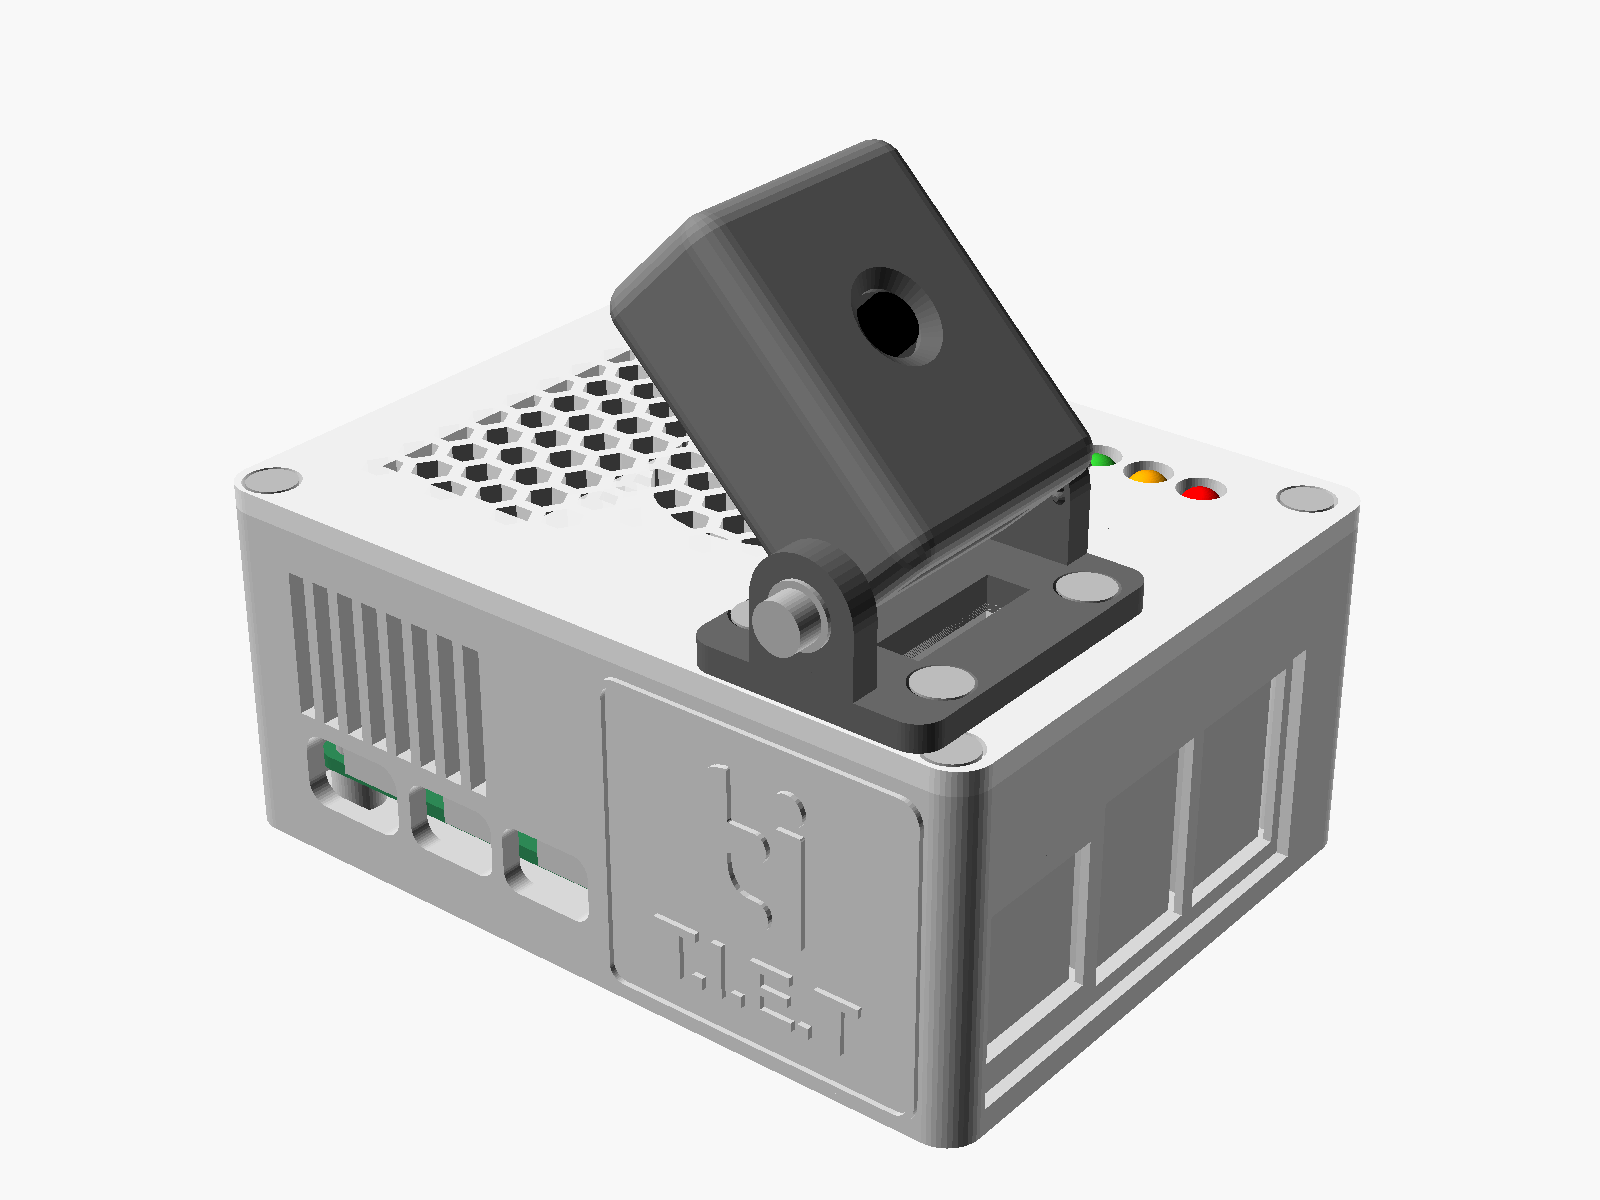
\includegraphics[width=0.32\textwidth]{figures/renders/1_assembled.png}\hfill
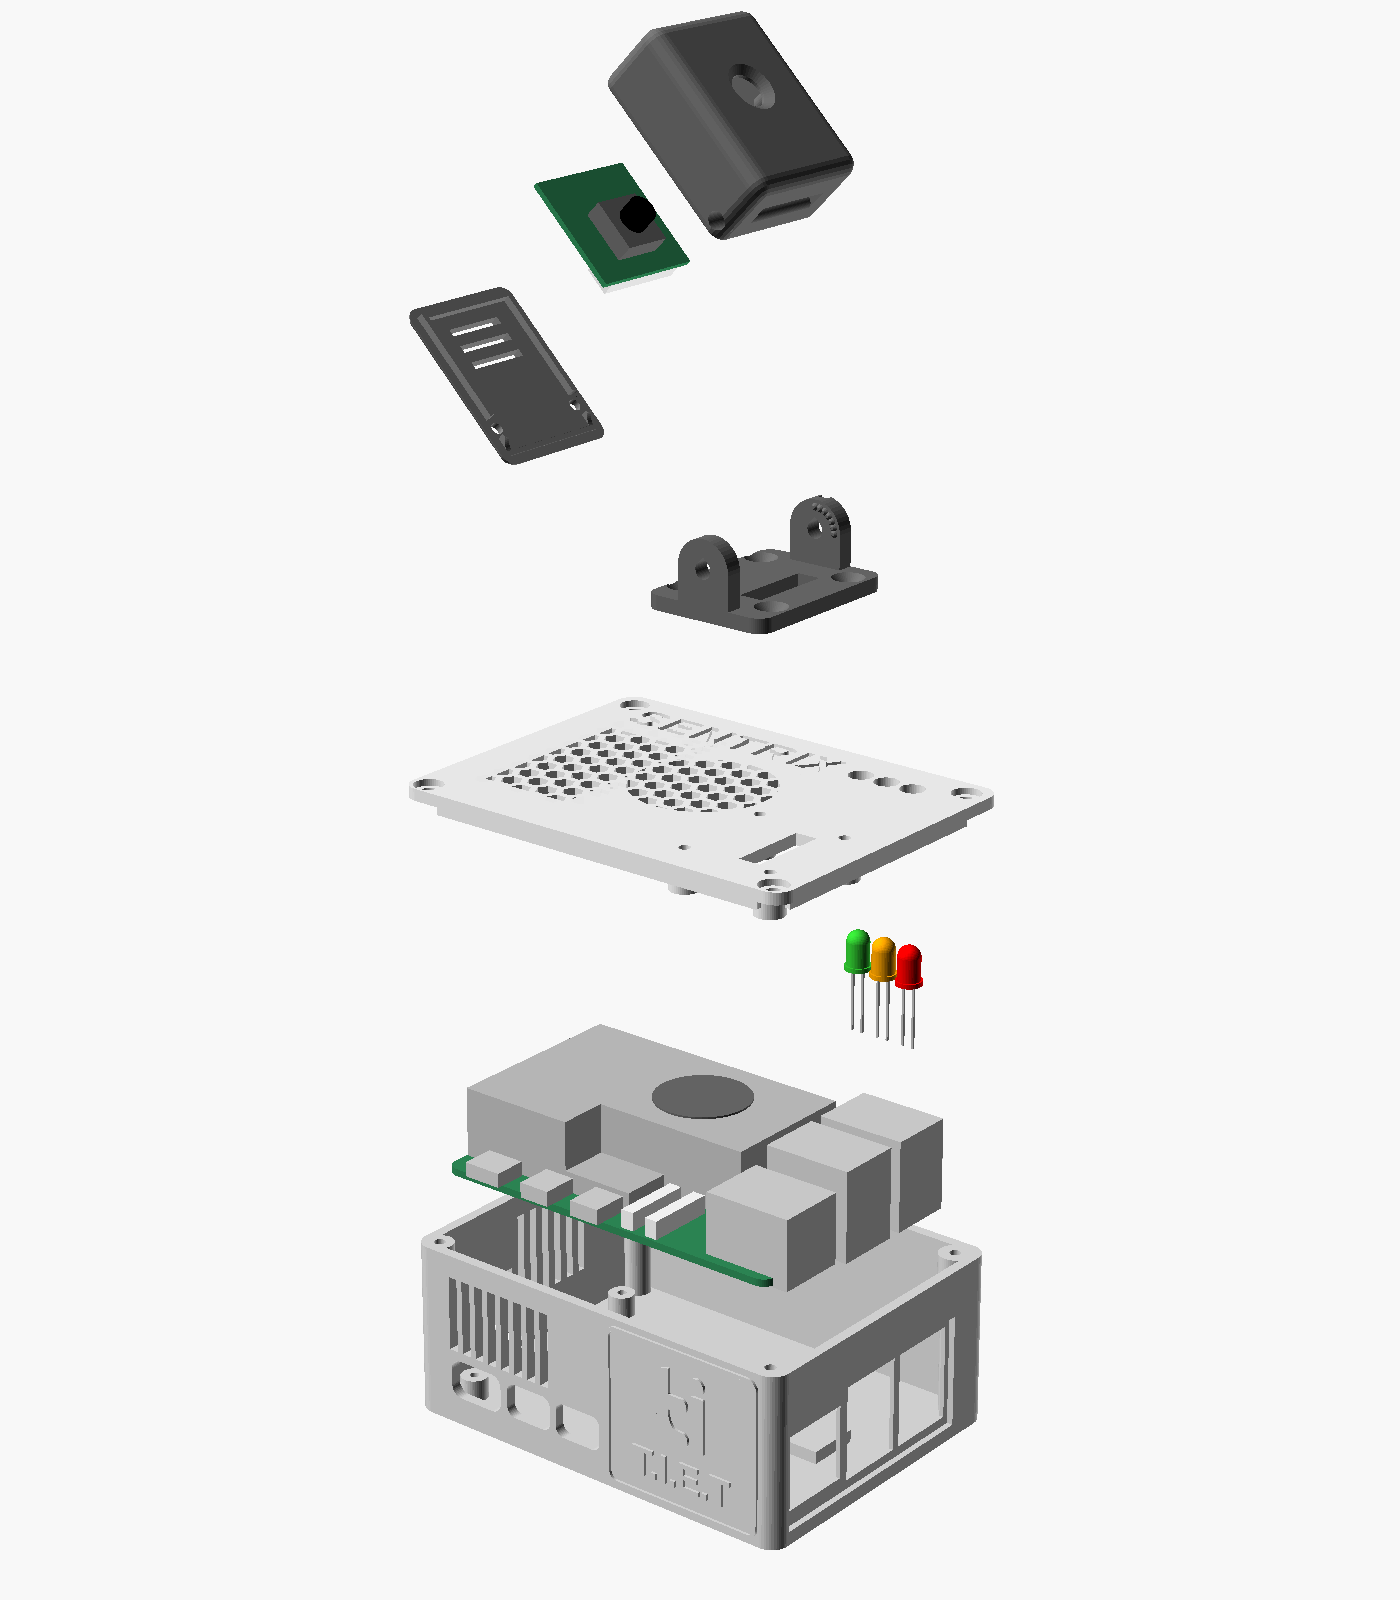
\includegraphics[width=0.32\textwidth]{figures/renders/2_exploded.png}\hfill
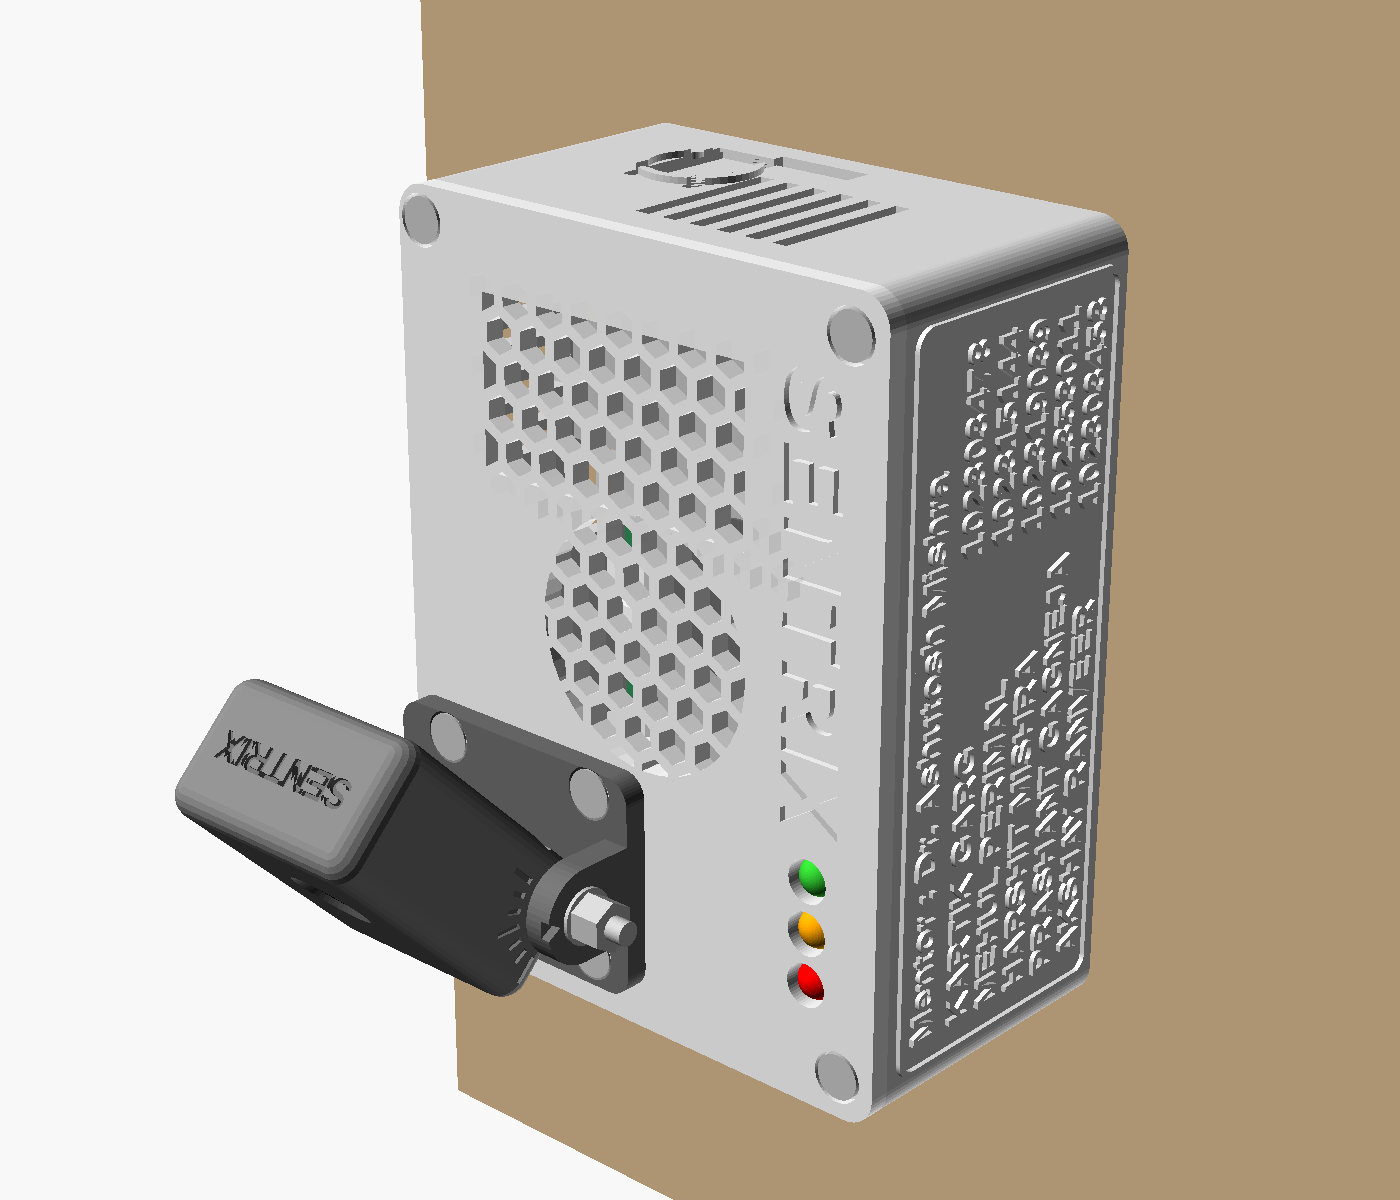
\includegraphics[width=0.32\textwidth]{figures/renders/9_wall_mounted.png}
\caption{Enclosure revision F: assembled, exploded, and wall-mounted with the camera end down}
\label{fig:enclosure}
\end{figure}

%==============================================================
\chapter{IMPLEMENTATION AND EXPERIMENTAL RESULTS}
\label{ch:impl}
%==============================================================

\section{Experimental Setup}
\label{sec:setup}

\tabref{tab:setup} lists the machines and environments used for development, training, evaluation and deployment.

\begin{table}[htbp]
\caption{Experimental and deployment environments}
\label{tab:setup}
\centering\tablefont
\begin{tabularx}{\textwidth}{|L{3.0cm}|Y|L{3.5cm}|}
\hline\rowhead
\thead{Machine} & \thead{Configuration} & \thead{Used for}\\ \hline
Development laptop & Intel Core i7-14650HX (24 threads), Windows 11, Python 3.14 virtual environment with CPU PyTorch & Evaluation, benchmarks (with 4 threads to mimic the Pi), tests, demo world\\ \hline
Training environment & Same laptop, NVIDIA RTX 4060 (8\,GB), separate Python 3.11 environment with CUDA PyTorch, Ultralytics, timm & Training the scene classifier, YOLO heads and slim heads\\ \hline
Raspberry~Pi~5 unit & 8\,GB, Raspberry~Pi~OS Trixie, Camera Module 3, Active Cooler; SENTRIX as a systemd user service in clip mode (ONNX, 320\,px object stage, fast lane, \code{buffalo\_s} faces) & Deployment in the demo room, on-device benchmarks, room calibration\\ \hline
Portal & Render web service (0.5 CPU, 512\,MB, Singapore) with a 1\,GB persistent disk, built from \code{deploy/portal/Dockerfile} & Accounts, owner prompts, Desk, tunnel for the demonstration\\ \hline
Test-mode demo world & \code{tools/demo\_reset.py} and \code{tools/demo\_run.py}: Portal and device on the laptop, a demo-reel camera playing recorded clips, every live switch forced off & End-to-end and browser tests, screenshots, rehearsals\\ \hline
\end{tabularx}
\end{table}

\paragraph{Evaluation tools.} Every measurement in this chapter was produced by a tool in the repository, and the report it wrote is committed under \code{training/runs/}:
\code{tools/eval\_custom\_frames.py} (per-image scores), \code{tools/replay\_custom\_videos.py} (the labelled videos through \code{Pipeline.process} at 6\,Hz with true timestamps, tick or clip mode, with the videos' own soundtracks), \code{tools/replay\_decisions.py} (re-decides a recorded live event log under the current rules), \code{tools/bench\_live.py} and \code{tools/bench\_clip.py} (the live loop with a video file as a 30\,fps camera), \code{tools/reid\_eval.py} (body re-identification pairs), \code{tools/eval\_models.py} (every vision model on every dataset it applies to), \code{tools/calibrate\_room.py} (per-room thresholds from the device's own log), and \code{tools/gate\_report.py} (the release gates). All of them run inside the side-effect-free harness described in Section~\ref{sec:investigative}, and all refuse the test video \code{wa02} unless it is evaluated as part of the full set.

%--------------------------------------------------------------
\section{Experimental Analysis}

\subsection{Data}
\label{sec:data}

\paragraph{Data sources.} Three kinds of data were used.
\begin{enumerate}
\item \textbf{Public corpora} for the first (v3) models: RWF-2000 violence clips \cite{cheng2021rwf}, Roboflow weapon and fire/smoke image sets, and AudioSet clips \cite{gemmeke2017audioset} for the first sound model. An audit of their splits (\code{tools/audit\_splits.py}) found that 52.7\,\% of the RWF-2000 validation rows shared source videos with training and that 12.2\,\% of the weapon and 20.0\,\% of the fire validation images were near-duplicates of training images, so their published scores are optimistic. They were used only for pre-training and rehearsal.
\item \textbf{The SENTRIX custom dataset}: ten videos recorded by the team---a bedroom with replica handguns and aerosol flame jets, and a corridor filmed by CCTV with a long stick, an assault and a bicycle theft. From them, 765 frames were hand-reviewed and labelled into five classes (\tabref{tab:dataset}); five more videos added in November bring the set to 977 frames (\tabref{tab:dataset-new}).
\item \textbf{Deployment logs}: the demonstration Pi's own event log in the demo room (about 12 hours, no threat present, and later its whole log from 23 October to 19 November) and the event log of the first live laptop session (18.3 minutes). These are used for calibration and regression, never for training.
\end{enumerate}

\begin{table}[htbp]
\caption{The custom dataset as used for the v4 models (the first ten videos; frames per class and split; splits by source video)}
\label{tab:dataset}
\centering\tablefont
\begin{tabular}{|l|c|c|c|c|}
\hline\rowhead
\thead{Class} & \thead{Train} & \thead{Validation} & \thead{Test} & \thead{Total}\\ \hline
Normal & 373 & 23 & 67 & 463\\ \hline
Fire & 11 & 6 & 0 & 17\\ \hline
Weapon (handgun, stick) & 144 & 55 & 26 & 225\\ \hline
Assault & 43 & 0 & 0 & 43\\ \hline
Robbery & 17 & 0 & 0 & 17\\ \hline
\textbf{Videos} & vid02, vid03, vid05, vid06, vid07, wa01, wa03 & gun, vid04 & wa02 & 10\\ \hline
\end{tabular}
\end{table}

\paragraph{Five videos added in November.} On 18 November 2026 the team added five videos: four masked-intruder scenes in the bedroom (a handgun pointed at a seated person, a knife attack, a beating with a metal flask, and a theft from the wardrobes) and one ordinary scene in a second room (\tabref{tab:dataset-new}). They were extracted with the original sampling rules and reviewed segment by segment, and they joined the training split; no video was held out. Grounding DINO proposed 27 boxes for them; 13 were kept after visual checks (7 pistol, 6 knife) and 14 rejected (a phone, a monitor). The dataset now holds 977 frames from fifteen videos and 180 checked boxes.

\begin{table}[htbp]
\caption{The five videos added on 18 November 2026 (all in the training split)}
\label{tab:dataset-new}
\centering\tablefont
\begin{tabularx}{\textwidth}{|l|Y|c|}
\hline\rowhead
\thead{Video} & \thead{Content} & \thead{Frames kept}\\ \hline
mmtheft & Masked intruder searches the shoe rack and wardrobes and leaves with items & 99 (robbery 62)\\ \hline
mmassault & Masked intruder strikes a person on the bed with a metal flask & 26 (assault 13)\\ \hline
mmgun & Handgun pointed at a seated person; a phone snatched at gunpoint & 23 (weapon 19)\\ \hline
mmknife & Knife attack on a person lying on the bed & 35 (weapon 28)\\ \hline
nvroom2 & Second room: three people, ordinary activity & 29 (normal)\\ \hline
\textbf{Total} & normal 90, weapon 47, assault 13, robbery 62 & \textbf{212}\\ \hline
\end{tabularx}
\end{table}

\paragraph{Cleaning and pruning.} Frames were sampled at 3--8\,fps, near-duplicates were dropped with a perceptual hash, and every kept frame was reviewed by a person. For video replay a label \emph{timeline} was built from every sampled frame: a kept frame carries its reviewed label; a dropped near-duplicate inherits its kept twin's label only if the twin is within 1\,s (a perceptual hash barely registers a flame jet, so a ``duplicate'' 5\,s away can differ in exactly the object that decides the label), otherwise it keeps its own segment label if that segment was confident ($\geq 0.7$), otherwise it is not scored. A replay tick is scored against the nearest sample within 0.25\,s.

\paragraph{Annotation and feature extraction.} Bounding boxes for the YOLO heads were proposed by Grounding DINO \cite{liu2024groundingdino} but kept only when gated by the reviewed frame label, a held-object check (the box must overlap a person's hands region) and a visual quality check: 167 boxes were kept and 16 rejected. The scene classifier sees each frame resized to 224\,px with ImageNet normalisation; the body embedder sees person crops padded to an aspect ratio of 0.5 and resized to 256$\times$128; the sound tagger sees 4\,s of 16\,kHz mono audio as a log-mel spectrogram. \figref{fig:datapipe} summarises the workflow.

\begin{figure}[htbp]
\centering
\resizebox{\textwidth}{!}{%
\begin{tikzpicture}[node distance=4mm, s/.style={draw, rounded corners=2pt, fill=sxlight, font=\scriptsize, align=center, text width=2.2cm, minimum height=10mm}, a/.style={-{Stealth[length=1.6mm]}, thick}]
\node[s] (v) {15 source videos\\(3 rooms)};
\node[s, right=of v] (f) {Frame sampling\\3--8\,fps};
\node[s, right=of f] (h) {Perceptual-hash\\de-duplication};
\node[s, right=of h] (r) {Human review:\\977 labelled frames};
\node[s, right=of r] (t) {Label timeline\\(1\,s rule)};
\node[s, below=6mm of r] (b) {Grounding DINO boxes,\\label-gated + QC\\(180 kept, 30 rejected)};
\node[s, below=6mm of t] (sp) {Split by video:\\7 train, 2 val, 1 test};
\node[s, left=of b] (tr) {Training: DINOv2 head,\\YOLO11n heads};
\node[s, left=of tr] (cv) {LOVO selection on\\9 videos, OOF\\temperature, thresholds};
\node[s, left=of cv] (te) {Confirm on val,\\report test once};
\draw[a] (v) -- (f); \draw[a] (f) -- (h); \draw[a] (h) -- (r); \draw[a] (r) -- (t); \draw[a] (t) -- (sp); \draw[a] (r) -- (b); \draw[a] (sp) -- (b); \draw[a] (b) -- (tr); \draw[a] (tr) -- (cv); \draw[a] (cv) -- (te);
\end{tikzpicture}}
\caption{Data workflow from the team's videos to selected models}
\label{fig:datapipe}
\end{figure}

\paragraph{Deployment-room data.} Because no model can be validated for a room it has never seen, the product records its own training data: the device administrator (or the owner, with a fresh password check) starts a recording on the dashboard; the device writes the camera's raw frames as a constant-frame-rate MJPEG video with the microphone's 16\,kHz audio muxed in, plus a JSON sidecar; recordings stop after 10 minutes, keep 2\,GB of disk free for evidence, are deleted after 14 days and can only be downloaded on the home network. Everyone filmed must consent.

\subsection{Performance Parameters}
\label{sec:perf-params}
\paragraph{Classification measures (per image or per tick).} Accuracy; \emph{macro-F1}, averaged only over the classes present in the split's ground truth (the test split has two, so a perfect model scores 1.0); threat recall and false-positive rate (normal versus any threat); and the area under the ROC curve (AUROC) \cite{fawcett2006roc} of a class probability against normal frames, which is threshold-free.

\paragraph{Alarm measures (per video replay).} An \emph{episode} is a contiguous run of ground-truth threat; it is detected at level $L$ if the matching class is committed at level $\geq L$ between its start and 1\,s after its end. A \emph{false onset} is a commit to level $\geq L$ on normal footage more than 1\,s from any episode. For $k$ false onsets in $T$ hours of normal footage the rate is $k/T$ with an exact Poisson 95\,\% interval; for $k=0$ the upper bound is
\begin{equation}
\lambda_{95} = \frac{-\ln(0.025)}{T} = \frac{3.689}{T}\ \text{per hour},
\end{equation}
so 3.7 minutes of normal footage can only show a rate below about 60 per hour. Recall per level carries a Clopper--Pearson interval \cite{clopper1934}. Latency is measured from the episode's start to the commit (median and 95th percentile).

\paragraph{Quality-of-service measures.} Preview frame rate (video fps), AI decision rate (Hz), tick latency and frame age (p50/p95), per-stage latency; on the Pi, clip compute time, the share of clips dropped because the previous clip was still running, and the age of a decision; for the Portal, the time from a scene to a pending request, from approval to dispatch, and the frame rate of remote video.

%--------------------------------------------------------------
\section{Working of the Project}

\subsection{Procedural Workflow}
\label{sec:workflow}
\figref{fig:workflow} shows the complete workflow of the product from installation to a closed incident. It has four phases.

\begin{figure}[htbp]
\centering
\resizebox{\textwidth}{!}{%
\begin{tikzpicture}[node distance=3.5mm, s/.style={draw, rounded corners=2pt, fill=sxlight, font=\scriptsize, align=center, text width=2.6cm, minimum height=11mm}, ph/.style={font=\scriptsize\bfseries, text=sxblue}, a/.style={-{Stealth[length=1.6mm]}, thick}]
\node[s] (p1) {Company provisions device:\\id, serial, claim code};
\node[s, below=of p1] (p2) {Customer activates,\\completes 7-step\\onboarding};
\node[s, below=of p2] (p3) {Device claimed; faces\\enrolled from the\\device camera};
\node[s, right=8mm of p1] (m1) {Capture frames;\\newest frame or\\4\,s clip analysed};
\node[s, below=of m1] (m2) {Models vote; evidence\\confirmed; TCI and\\level committed};
\node[s, below=of m2] (m3) {Level 3: snapshot,\\encrypted evidence,\\assistance request};
\node[s, right=8mm of m1] (r1) {Owner prompted:\\Portal, device screen,\\Telegram, e-mail};
\node[s, below=of r1] (r2) {Approve / false alarm\\(PIN) / checking /\\duress / no answer};
\node[s, below=of r2] (r3) {Safety defaults:\\L4/L5, fire after\\2\,min, device offline};
\node[s, right=8mm of r1] (c1) {Contacts and Desk\\receive the dispatch\\package};
\node[s, below=of c1] (c2) {Desk acknowledges,\\owner sees ``handling''};
\node[s, below=of c2] (c3) {Desk resolves:\\verdict recorded,\\evidence reviewed};
\node[ph, above=1mm of p1] {1. Set-up};
\node[ph, above=1mm of m1] {2. Detection};
\node[ph, above=1mm of r1] {3. Owner decision};
\node[ph, above=1mm of c1] {4. Response};
\draw[a] (p1) -- (p2); \draw[a] (p2) -- (p3); \draw[a] (p3.east) -- ++(4mm,0) |- (m1.west);
\draw[a] (m1) -- (m2); \draw[a] (m2) -- (m3); \draw[a] (m3.east) -- ++(4mm,0) |- (r1.west);
\draw[a] (r1) -- (r2); \draw[a] (r2) -- (r3); \draw[a] (r2.east) -- ++(4mm,0) |- (c1.west);
\draw[a] (r3.east) -- ++(2mm,0) |- (c1.south west);
\draw[a] (c1) -- (c2); \draw[a] (c2) -- (c3);
\end{tikzpicture}}
\caption{Procedural workflow of SENTRIX, from installation to a closed incident}
\label{fig:workflow}
\end{figure}

\textbf{Set-up.} The company provisions a device with \code{tools/provision\_device.py}, which creates its identity (device id, serial number, claim code and the credential the device uses on its link) and prints a label with a QR code. The administrator creates the customer on the Portal's admin console and prints a welcome letter with a single-use activation code. The customer activates the account, sets a password and completes the onboarding wizard: profile, address with entry notes for responders, household (adults, seniors, children, pets, medical and accessibility notes), emergency contacts---each confirms by a consent link before receiving anything---claiming the device with its serial and claim code, alert channels with the SOS PIN, an optional duress PIN and the answer window, and finally consent and a preview of exactly what contacts would receive. Residents are enrolled from the device's own camera, with quality checks (one face, at least 80\,px, sharp, well lit, not already enrolled under another name).

\textbf{Detection.} The device then monitors continuously. On a laptop each tick analyses the newest frame at up to 6\,Hz; on the Pi a 4\,s clip is analysed every 2\,s while the fast lane checks every fourth frame. The models produce votes; the evidence rules confirm them and decide which modalities agree; the TCI and the level policy commit a level; an incident opens with a frozen peak snapshot. At Level~3 the device stores a snapshot, seals an encrypted evidence bundle (with the 4\,s before the trigger in clip mode) and, for an alarm class, triggers one assistance request. Everything is written to the event log as it happens, and the device screen, the LEDs and every connected viewer update within the same tick.

\textbf{Owner decision.} The request is mirrored to the Portal over the link. The owner is asked on the Portal (a red bar on every page and a full alert screen), on the device screen (a full-screen takeover with a PIN pad) and by Telegram and e-mail; SMS from the 4G modem is used when the device is offline or the prompt is unseen after 10 minutes. The owner approves (choosing Police, Fire or Medical), marks a false alarm with the SOS PIN, or taps ``I'm checking''. If the owner does not answer, reminders follow at 2, 5, 10 and 20 minutes and a warning 5 minutes before the window closes; at the end the request expires as ``unanswered''. Meanwhile the safety defaults may already have alerted the contacts.

\textbf{Response.} On approval the dispatch package---address, entry notes, household, the snapshot, the detection's timeline---goes to the confirmed contacts and to the SENTRIX Desk. The Desk operator acknowledges the request (the owner's screen changes to ``The SENTRIX Desk is handling it''), can record that 112 was called, and closes the request with an outcome (for example ``help arrived'' or ``false alarm confirmed''), which sets the incident's verdict. Verdicts and the logged votes are the labels from which a future fitted fusion model can be trained.

\subsection{Algorithmic Approaches Used}
\label{sec:algorithms}

\paragraph{Evidence confirmation and the TCI.} \algref{alg:evidence} is executed for every tick (or every clip). It implements Equations~(\ref{eq:strength})--(\ref{eq:tci}). The key property is that only a \emph{fresh} evaluation is pushed into a confirmation window, so a model that runs every second tick, or a cached result, cannot confirm itself; and that a modality only counts once, so two classifiers on the same pixels never corroborate each other.

\begin{algorithm}[htbp]
\caption{Confirmed per-class evidence and the Threat Confidence Index}
\label{alg:evidence}
\small
\begin{algorithmic}[1]
\Require votes $V=\{(\text{source}, c, v, \theta, \text{fresh})\}$, time $t$, persons seen at $t_p$, unknown-person dwell $d_u$
\Ensure TCI, leading class, evidence state, contributions
\ForAll{$(s, c, v, \theta, \text{fresh}) \in V$}
  \If{$v$ not finite \textbf{or} $\theta \notin (0,1)$} mark vote \emph{gated}; \textbf{continue} \EndIf
  \If{fresh} push $[v \geq \theta]$ into window $W_{s,c}$ (drop entries older than 3\,s) \EndIf
  \State $\text{confirmed}_{s,c} \gets$ at least 2 of the last 3 entries of $W_{s,c}$ are true
  \If{$c = \text{weapon}$ \textbf{and} $t - t_p > 2$\,s} $\text{confirmed}_{s,c} \gets$ false \Comment{person gate} \EndIf
\EndFor
\ForAll{class $c$}
  \State $M \gets \{\text{modality}(s) : \text{confirmed}_{s,c}\}$ with strength $s_m = \max s(v,\theta)$ per modality
  \If{$M = \emptyset$} $e_c \gets 0.19 \cdot \min(v_{\max}/\theta, 1)$
  \ElsIf{$M = \{\text{audio}\}$} $e_c \gets \min(\cdot, \text{L2 cap})$ \Comment{audio alone}
  \ElsIf{$|M| = 1$} $e_c \gets 0.45 + 0.17\, s_{(1)}$
  \Else\ $e_c \gets \min(0.70 + 0.25\, s_{(2)}, 0.95)$; \textbf{if} $|M|=3$ and audio strength $\geq 0.3$ \textbf{then} $e_c \gets \max(e_c, 0.86)$
  \EndIf
  \If{$c$ is experimental \textbf{or} (fight \textbf{and not} video+aggression) \textbf{or} banter} $e_c \gets \min(e_c, \text{L2 cap})$ \EndIf
\EndFor
\State $u \gets 0.30$ \textbf{if} $d_u \geq$ dwell (3\,s armed, 10\,s home) \textbf{else} $0$
\State \Return $\mathrm{TCI} = \max(\max_c e_c, u)$, the arg-max class, and every vote with its role
\end{algorithmic}
\end{algorithm}

\paragraph{Level policy.} \algref{alg:policy} turns the TCI into a committed level. A separate timer per threshold means that a ramp from Level~1 to Level~5 commits each level as it is earned rather than restarting a single dwell at every band change.

\begin{algorithm}[htbp]
\caption{Level policy with per-threshold timers}
\label{alg:policy}
\small
\begin{algorithmic}[1]
\Require TCI $x$ at time $t$; thresholds $\tau_2..\tau_5 = 0.20, 0.40, 0.65, 0.85$; committed level $L$
\ForAll{$k \in \{2,3,4,5\}$}
  \If{$x \geq \tau_k$} start timer $T_k$ if stopped; increment observations $n_k$
  \Else\ stop $T_k$; $n_k \gets 0$ \EndIf
\EndFor
\State $L^\uparrow \gets \max\{k : x \geq \tau_k \wedge (k \leq 3 \vee (T_k \geq 0.6\,\text{s} \wedge n_k \geq 2))\}$
\If{$L^\uparrow > L$} $L \gets L^\uparrow$; record the commit \Comment{escalate}
\ElsIf{no threshold $\geq L$ has been supported for 5\,s} $L \gets$ highest supported level (at least 1) \Comment{step down}
\EndIf
\State \Return $L$
\end{algorithmic}
\end{algorithm}

\paragraph{Clip engine.} \algref{alg:clip} is the Raspberry~Pi strategy. The cascade spends compute only when there is something to look at: in a still, empty room only the gate runs, but a full cascade is forced at least every 10\,s so that a flame in an empty room is never missed.

\begin{algorithm}[htbp]
\caption{Clip engine cascade (every 2\,s) and fast lane (every 4th frame)}
\label{alg:clip}
\small
\begin{algorithmic}[1]
\Procedure{AnalyseClip}{ring buffer of the last 4\,s}
  \State $g \gets$ motion energy $>0.015$ \textbf{or} audio RMS above floor \textbf{or} PIR/door event \textbf{or} alarm active \textbf{or} 10\,s since last full cascade
  \If{\textbf{not} $g$} \Return no-change result \EndIf
  \State $K \gets$ 4 uniform + 2 highest-motion keyframes; reuse results for keyframes shared with the previous clip
  \State run person, weapon, fire heads (320\,px) on new keyframes \Comment{S1}
  \If{person or fire candidate} DINOv2 on up to 2 new keyframes \EndIf \Comment{S2}
  \If{persons present} face check (at most every 2\,s) \EndIf \Comment{S3}
  \If{$\geq 2$ persons \textbf{and} motion $\geq 0.10$} action model on the two halves \EndIf \Comment{S4}
  \State classify the clip's own 4\,s audio \Comment{S5}
  \State confirm a class on 2 keyframes of one track (fire: one region); \Call{Evidence}{}; \Call{LevelPolicy}{} \Comment{S6}
\EndProcedure
\Procedure{FastLane}{frame $i$}
  \If{$i \bmod 4 = 0$} run weapon and fire heads at 320\,px
    \If{same track hit on 2 consecutive passes \textbf{and} (fire \textbf{or} person seen)} raise Level 3 now \EndIf
  \EndIf
\EndProcedure
\end{algorithmic}
\end{algorithm}

\paragraph{Body re-identification for residents.} \algref{alg:reid} decides when a track whose face is not visible may still be treated as an enrolled resident at home. The bar of 0.87 was chosen by a rule fixed in advance (Section~\ref{sec:results}): on fourteen videos it accepts 30\,\% of same-person cases and 0.020\,\% of different-people cases.

\begin{algorithm}[htbp]
\caption{Resident identity from body appearance (home mode only)}
\label{alg:reid}
\small
\begin{algorithmic}[1]
\Require track $k$ without a face verdict; OSNet embedding $b_k$; looks $\mathcal{L}_r$ (last 20 face-verified bodies per resident, 30 min)
\If{armed mode \textbf{or} track $k$'s face was seen and failed} \Return unverified \EndIf
\ForAll{resident $r$ not already authorised by face on another track in view}
  \State $m_r \gets \max_{\ell \in \mathcal{L}_r} \cos(b_k, \ell)$
\EndFor
\State $r^\star \gets \arg\max_r m_r$; \ \ $\Delta \gets m_{r^\star} - \max_{r \neq r^\star} m_r$
\If{$m_{r^\star} \geq 0.87$ \textbf{and} $\Delta \geq 0.05$ on this check \textbf{and} the previous one} \Return authorised as $r^\star$ (via appearance) \EndIf
\State \Return unverified
\end{algorithmic}
\end{algorithm}

\paragraph{The assistance request sweeper.} \algref{alg:sweeper} runs every few seconds on the device (and on the Portal when it holds authority for an offline device). It is a pure function of the request's snapshot and the time, so it is tested by ``time travel'': the tests move a fake clock and check every message the sweeper decides to send.

\begin{algorithm}[htbp]
\caption{Assistance request sweeper (owner timeline and safety defaults)}
\label{alg:sweeper}
\small
\begin{algorithmic}[1]
\Require open request $q$ with creation time $t_0$, frozen policy (window $w$, contacts, safety defaults), now $t$
\If{$q$ is PENDING}
  \ForAll{reminder offset $o \in \{2, 5, 10, 20\}$ min with $t - t_0 \geq o$ not yet sent} queue one reminder (collapse overdue ones) \EndFor
  \If{prompt unseen \textbf{and} $t - t_0 \geq 10$ min} queue owner SMS \EndIf
  \If{$t \geq t_0 + w - 5$ min} queue the lapse warning \EndIf
  \If{$t \geq t_0 + w$} transition to EXPIRED (``unanswered''); \Return \EndIf
\EndIf
\State $(\delta, \text{reason}) \gets$ \Call{ContactsDelay}{type, peak level} \Comment{0 for L4/L5 or duress; 2 min for fire}
\If{$\delta$ defined \textbf{and} $t - t_0 \geq \delta$ \textbf{and} contacts not yet notified} alert confirmed contacts (flag \emph{contacts\_notified}) \EndIf
\If{$q$ on the help path \textbf{and} no channel delivered within 60\,s} warn the owner ``not delivered''; after the delivery window, FAILED \EndIf
\If{$q$ on the help path for 24\,h without a resolve} stale close \EndIf
\end{algorithmic}
\end{algorithm}

\paragraph{The send guard.} Every message, from any channel on either side, passes one function that re-reads the configuration on each call: refuse an emergency number; refuse unless the global live switch and the channel's switch are both on; in test mode refuse any recipient not on the allowlist and prefix the text with the test banner; otherwise send. A refusal is recorded as SUPPRESSED with its reason, so a whole alarm can be rehearsed on the real code without contacting anyone.

\subsection{Project Deployment}
\label{sec:deployment}

\figref{fig:deployment} shows the deployment of the demonstration system.

\begin{figure}[htbp]
\centering
\resizebox{\textwidth}{!}{%
\begin{tikzpicture}[node distance=4mm, nd/.style={draw, thick, fill=sxhead!60, align=left, font=\scriptsize, inner sep=4pt}, art/.style={draw, fill=white, font=\tiny, align=left, text width=3.1cm, inner sep=2pt}, a/.style={-{Stealth[length=1.6mm]}, thick}]
\node[art] (a1) at (0,0) {\textbf{sentrix.service} (systemd user unit, watchdog 30\,s, pin forced low after exit)};
\node[art, below=1.5mm of a1] (a2) {Python venv (system site packages: Picamera2, lgpio) + \texttt{pi.env} profile: clip mode, ONNX, 320\,px, fast lane};
\node[art, below=1.5mm of a2] (a3) {models/ (DINOv2 delta, YOLO11n, OSNet, PANNs) and var/ (SQLite, events, evidence, faces)};
\node[art, below=1.5mm of a3] (a4) {Local Console on :8000, firewalled to the home subnet (ufw)};
\node[draw, thick, fit=(a1)(a4), inner sep=5pt, label={[font=\scriptsize\bfseries, align=center]above:$\ll$device$\gg$ Raspberry Pi 5 (demo room)}] (pi) {};
\node[art] (b1) at (8.0,0) {\textbf{Docker container}: \texttt{python -m sentrix\_portal} (non-root after start-up), health check /healthz};
\node[art, below=1.5mm of b1] (b2) {/data disk (1\,GB): SQLite, keys, files};
\node[art, below=1.5mm of b2] (b3) {Link hub /device/v1/link, tunnel /d/\{device\}/, workers (hub watcher, cloud SOS timers, notifications, retention)};
\node[draw, thick, fit=(b1)(b3), inner sep=5pt, label={[font=\scriptsize\bfseries]above:$\ll$cloud$\gg$ Render web service (Singapore)}] (rd) {};
\node[nd] (wifi) at (4.0,-4.6) {Home Wi-Fi router\\(phone hotspot as fallback)};
\node[nd] (tg) at (8.0,-4.6) {Telegram Bot API\\(polling)};
\node[nd] (ph) at (11.6,-2.0) {Phones and browsers:\\owner, contact, Desk,\\admin};
\node[nd] (lap) at (0,-4.6) {Laptop on the LAN\\(device admin,\\recording downloads)};
\draw[a] (pi.south east) -- (wifi.north west);
\draw[a] (wifi.north east) -- node[right, font=\tiny, pos=0.4]{outbound WSS (TLS)} (rd.south west);
\draw[a, <->] (rd.south) -- (tg.north);
\draw[a, <->] (rd.east) -- node[below, font=\tiny, sloped]{HTTPS} (ph.north west);
\draw[a, <->] (tg.east) -- (ph.south west);
\draw[a, <->] (lap.north) -- node[left, font=\tiny]{HTTP, LAN only} (pi.south);
\end{tikzpicture}}
\caption{Deployment diagram of the demonstration system}
\label{fig:deployment}
\end{figure}

\paragraph{Device.} On the Pi, \code{deploy/pi5/install\_pi.sh} installs the system packages (Picamera2, lgpio, ffmpeg), creates the virtual environment with system site packages, removes the conflicting full OpenCV build, merges the \code{pi.env} profile into \code{.env}, installs the systemd unit with its watchdog and journald drop-ins, sets \code{gpio=17=op,dl} in \code{config.txt} so the siren pin is low from power-on, configures NetworkManager failover profiles and the \code{ufw} firewall. The demo unit runs SENTRIX as a systemd \emph{user} service with lingering enabled, so it starts at boot and the dashboard opens at desktop login. The device is provisioned (\code{SX5-000001}), linked to the Portal (\code{SENTRIX\_LINK\_ENABLED=1}, the Portal URL and the identity in \code{var/link/}) and claimed by the owner's account. Per-room thresholds live in \code{var/calibration/scene.json} (weapon 0.75, fire 0.70 for the demo room).

\paragraph{Portal.} The Portal is deployed from a Render Blueprint (\code{render.yaml}): one web service in Singapore built from \code{deploy/portal/Dockerfile}, a 1\,GB disk on \code{/data}, keys generated by Render and secrets typed in by the team. The container starts as root only to hand the volume to an unprivileged user and then drops root for good. The first company administrator is created from \code{PORTAL\_BOOTSTRAP\_ADMIN}. The service is suspended between evaluation sessions to save cost. For a long-term deployment, \code{deploy/portal/} also contains a Docker Compose stack with Postgres on an internal network, Caddy for HTTPS, and backup and restore scripts.

\paragraph{Alerts.} A Telegram bot (created with BotFather, polling mode) carries the owner's question and the contacts' alerts; in test mode only the team's two allowlisted chats can receive them. E-mail through an HTTPS API and SMS through the 4G modem use the same router, outbox and guard.

\subsection{System Screenshots}
\label{sec:screens}
The screenshots below were captured from the product running in its test-mode demo world (Portal and device on one laptop, the held-out handgun clip played through the demo-reel camera, every live switch off); the detections are real outputs of the shipped models, and the people in the frames are team members from the custom dataset.

\begin{figure}[H]
\centering
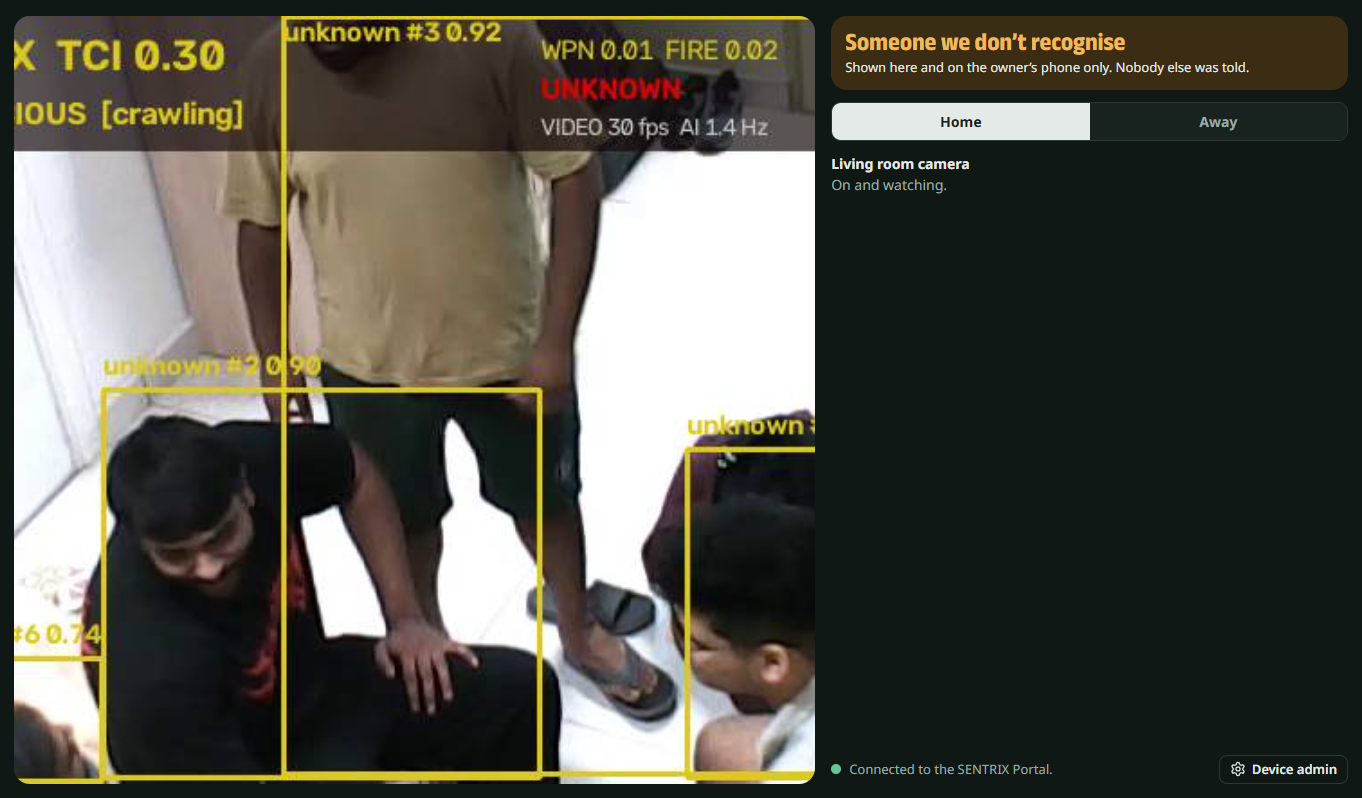
\includegraphics[width=0.49\textwidth]{figures/screens_c/dev_wall_idle.png}\hfill
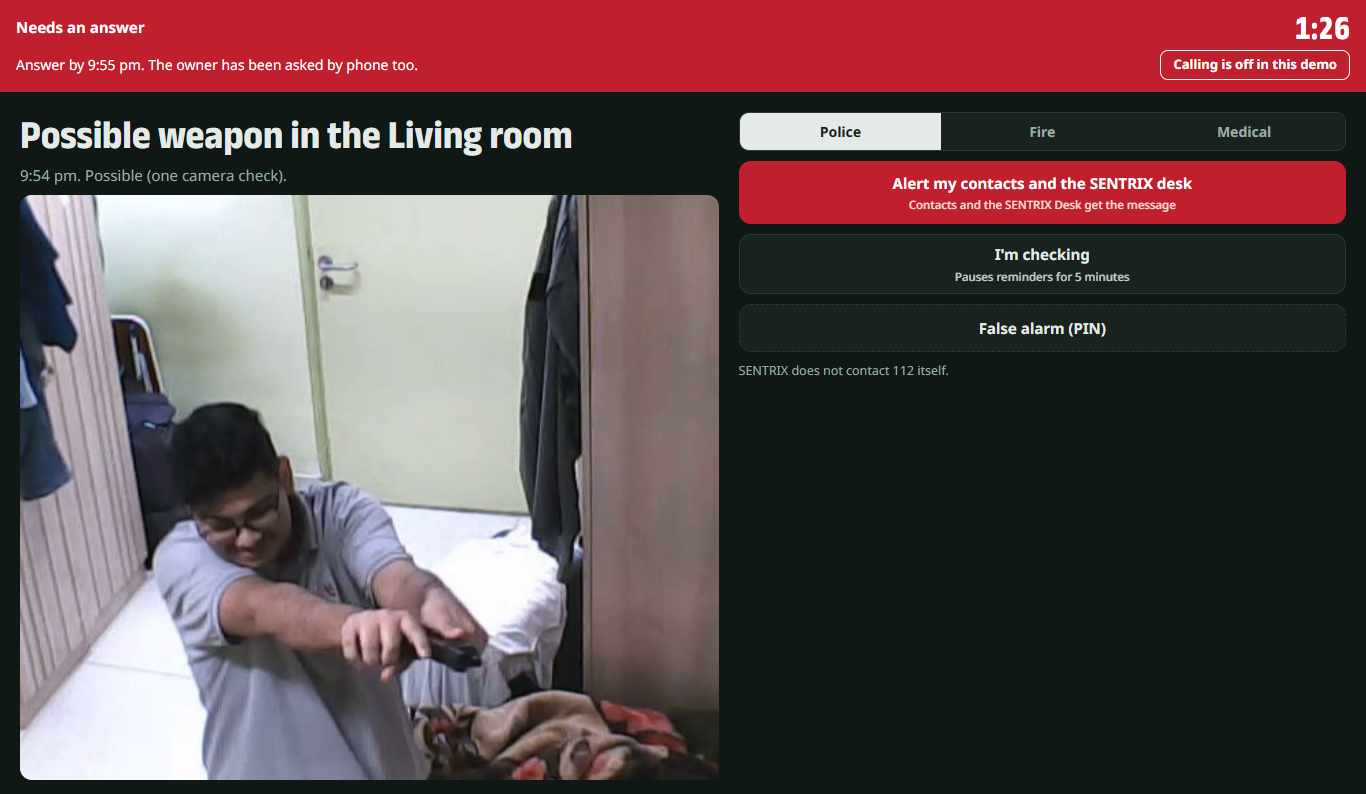
\includegraphics[width=0.49\textwidth]{figures/screens_c/dev_wall_alert.png}
\caption{Device screen: monitoring with tracked people labelled ``unknown'' (left) and the alert takeover after the handgun was confirmed, with countdown and answers (right)}
\label{fig:scr-wall}
\end{figure}

\begin{figure}[H]
\centering
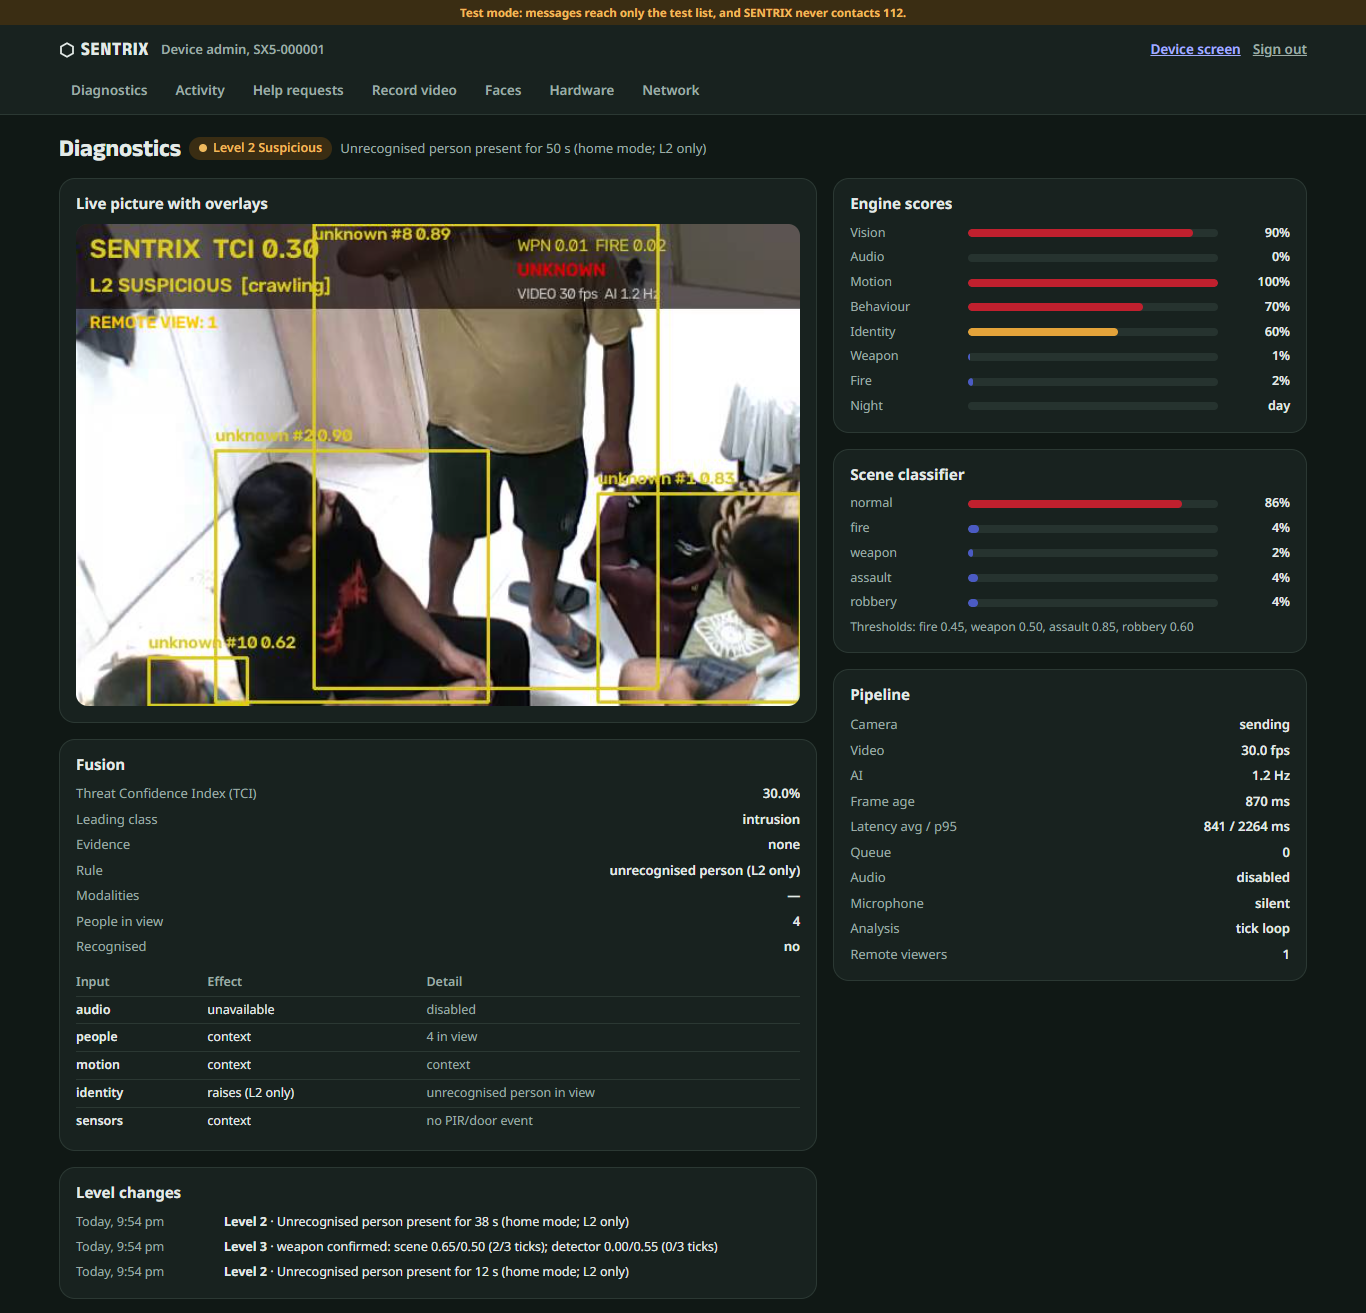
\includegraphics[width=0.92\textwidth]{figures/screens_c/dev_diagnostics.png}
\caption{Device administration, Diagnostics: live picture with overlays, model scores, scene probabilities with thresholds, the fusion result with the contribution of each input, and the level changes}
\label{fig:scr-diag}
\end{figure}

\begin{figure}[H]
\centering
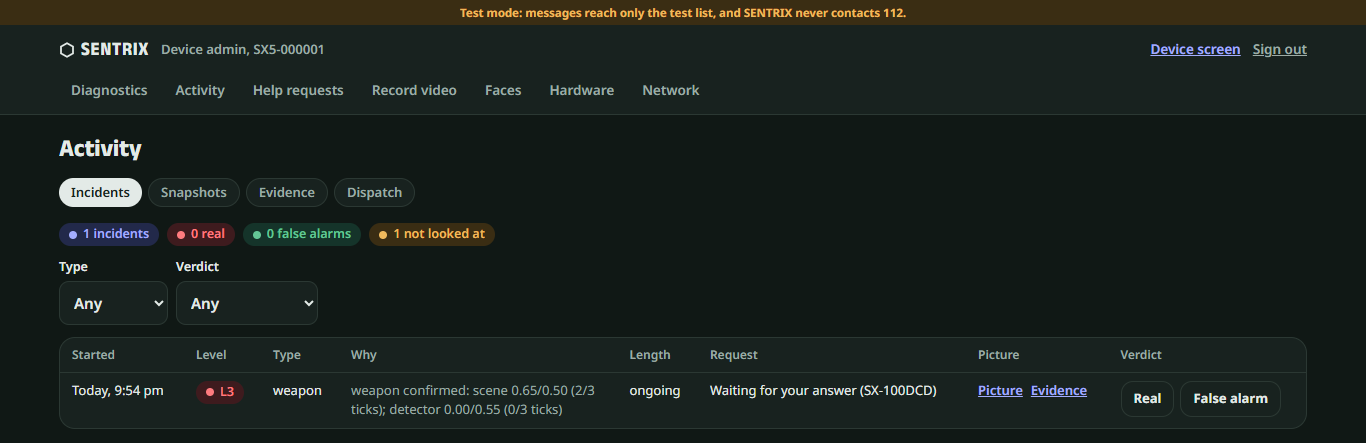
\includegraphics[width=0.49\textwidth]{figures/screens_c/dev_activity.png}\hfill
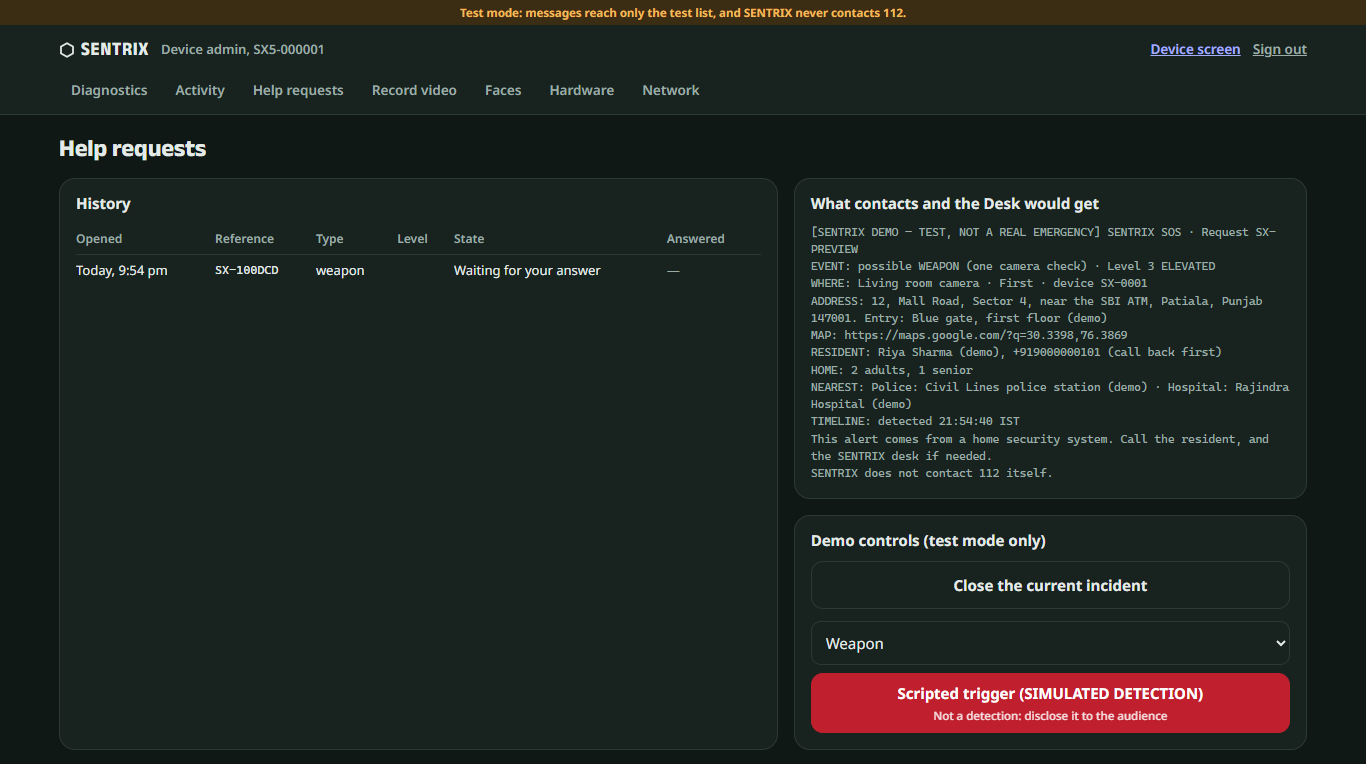
\includegraphics[width=0.49\textwidth]{figures/screens_c/dev_sos.png}
\caption{Device administration: Activity with the incident, its picture, evidence and verdict buttons (left); Help requests with the exact message contacts and the Desk would receive (right)}
\label{fig:scr-devadmin}
\end{figure}

\begin{figure}[H]
\centering
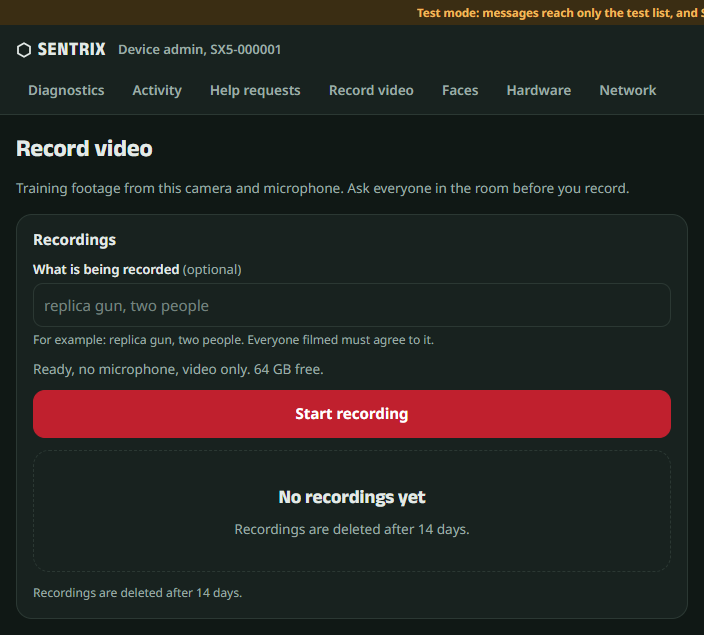
\includegraphics[width=0.36\textwidth]{figures/screens_c/dev_recordings.png}\hfill
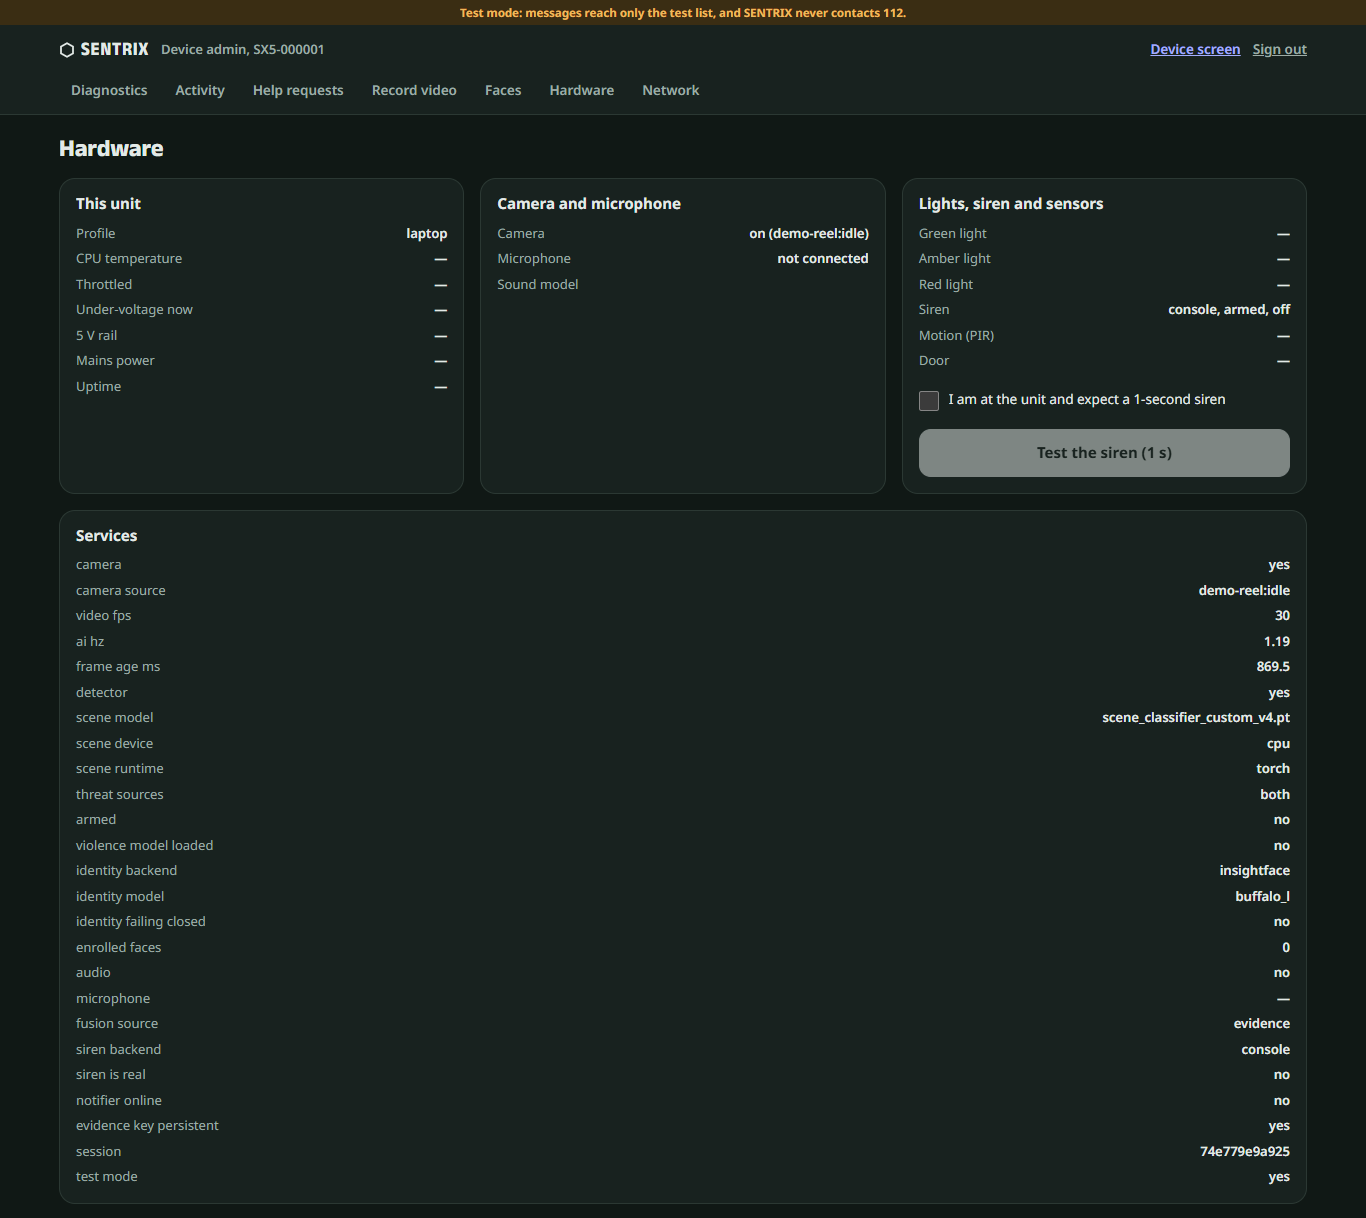
\includegraphics[width=0.62\textwidth]{figures/screens_c/dev_hardware.png}
\caption{Device administration: Record video for training data (left) and Hardware with services, LEDs, siren and sensors (right)}
\label{fig:scr-devhw}
\end{figure}

\begin{figure}[H]
\centering
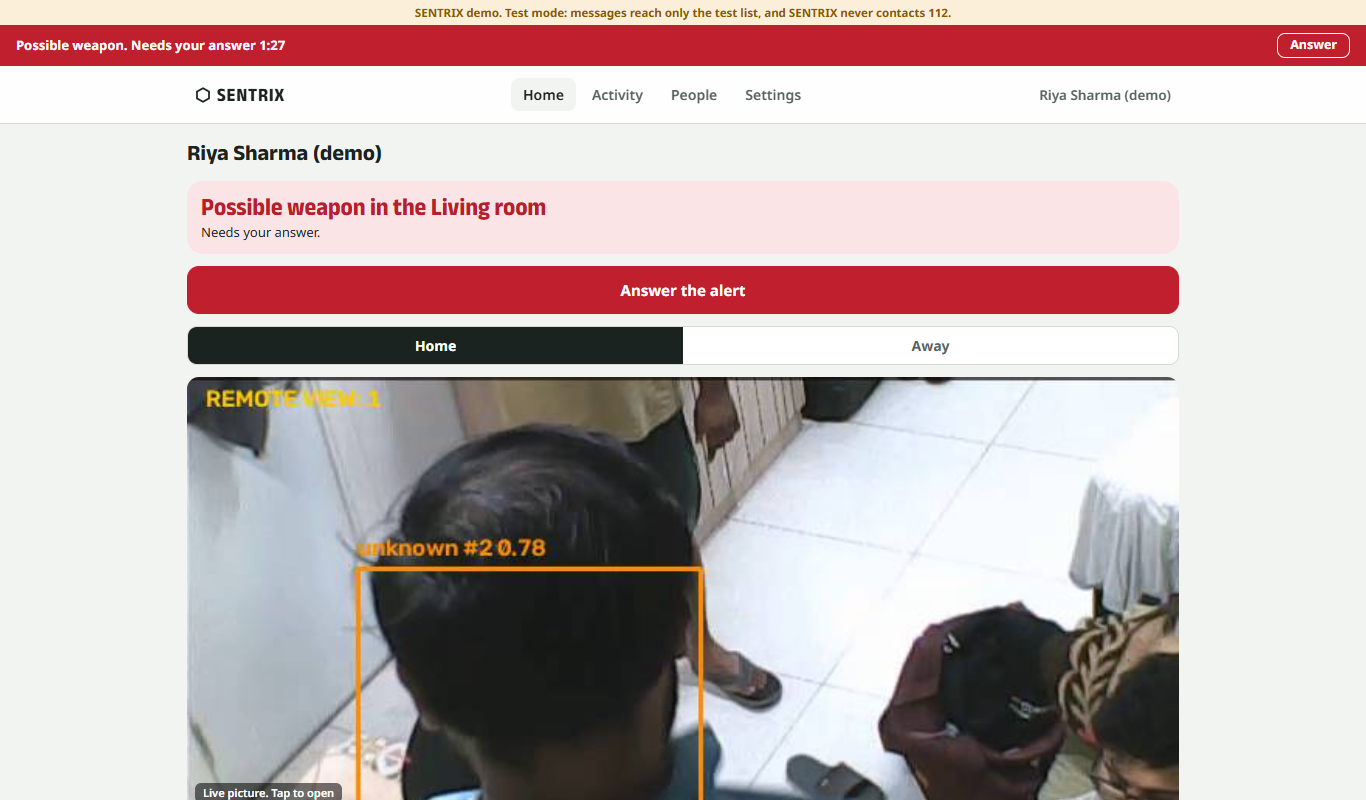
\includegraphics[width=0.60\textwidth]{figures/screens_c/portal_home_alert.png}\hfill
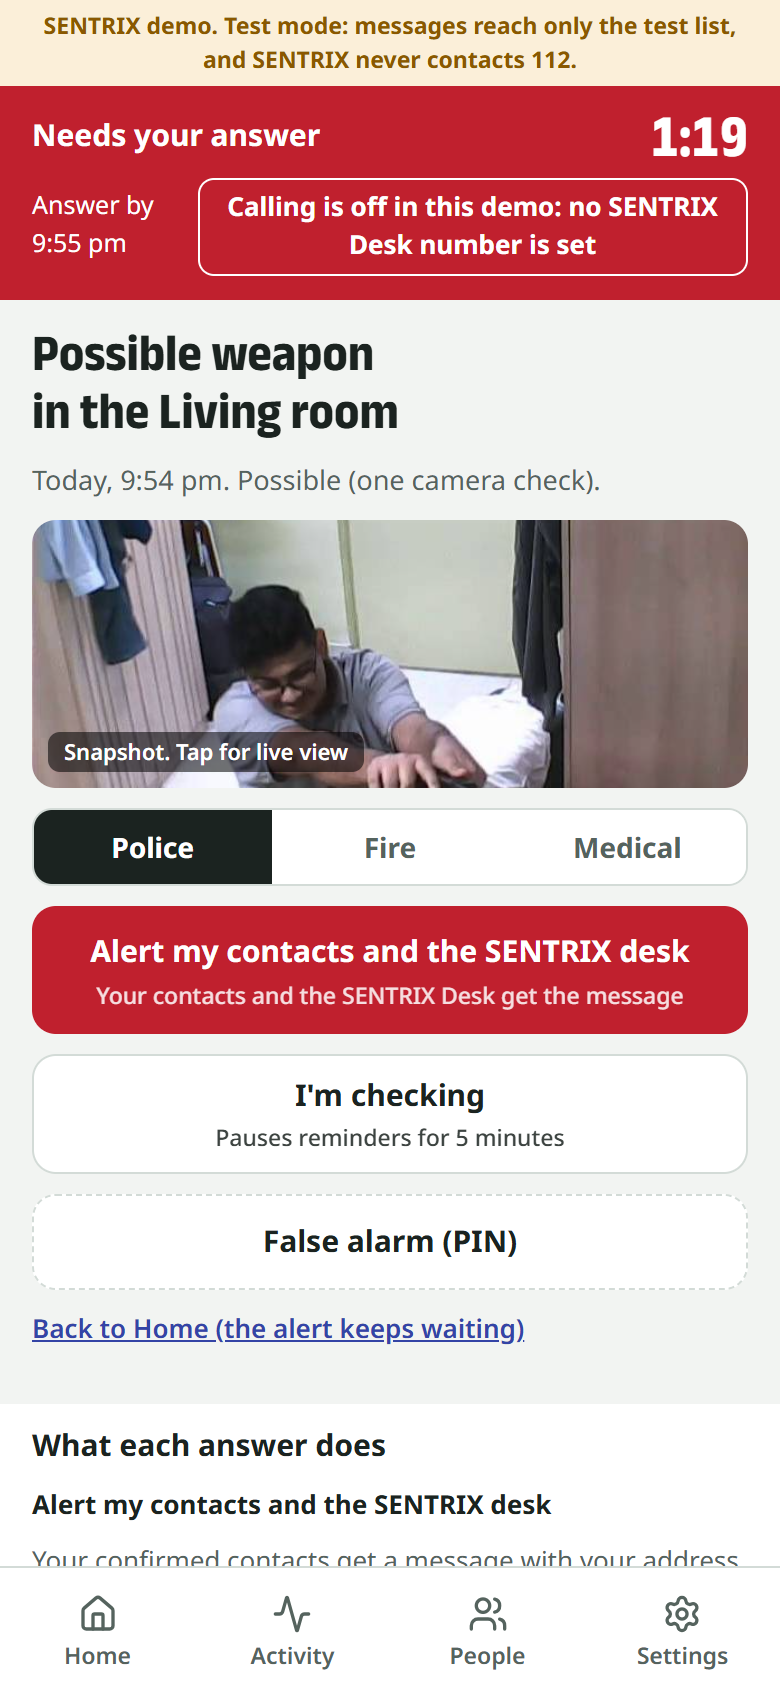
\includegraphics[width=0.36\textwidth]{figures/screens_c/portal_alert_phone.png}
\caption{Portal: the owner's home page with the red alert bar (left) and the alert screen on a phone, answers first (right)}
\label{fig:scr-alert}
\end{figure}

\begin{figure}[H]
\centering
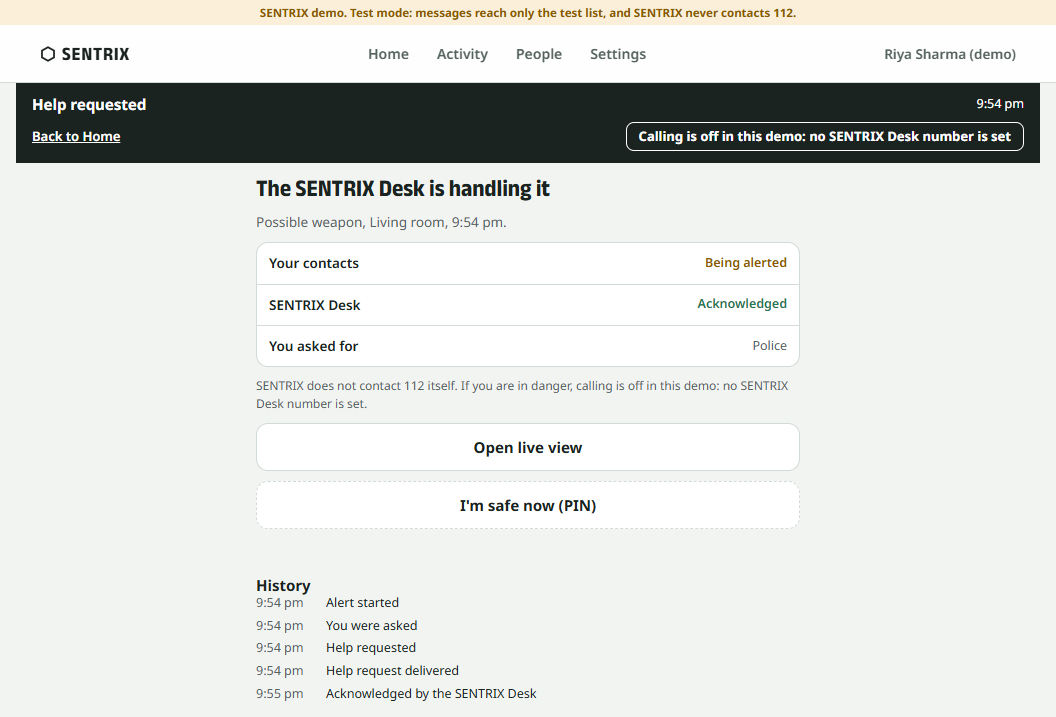
\includegraphics[width=0.49\textwidth]{figures/screens_c/portal_alert_ack.png}\hfill
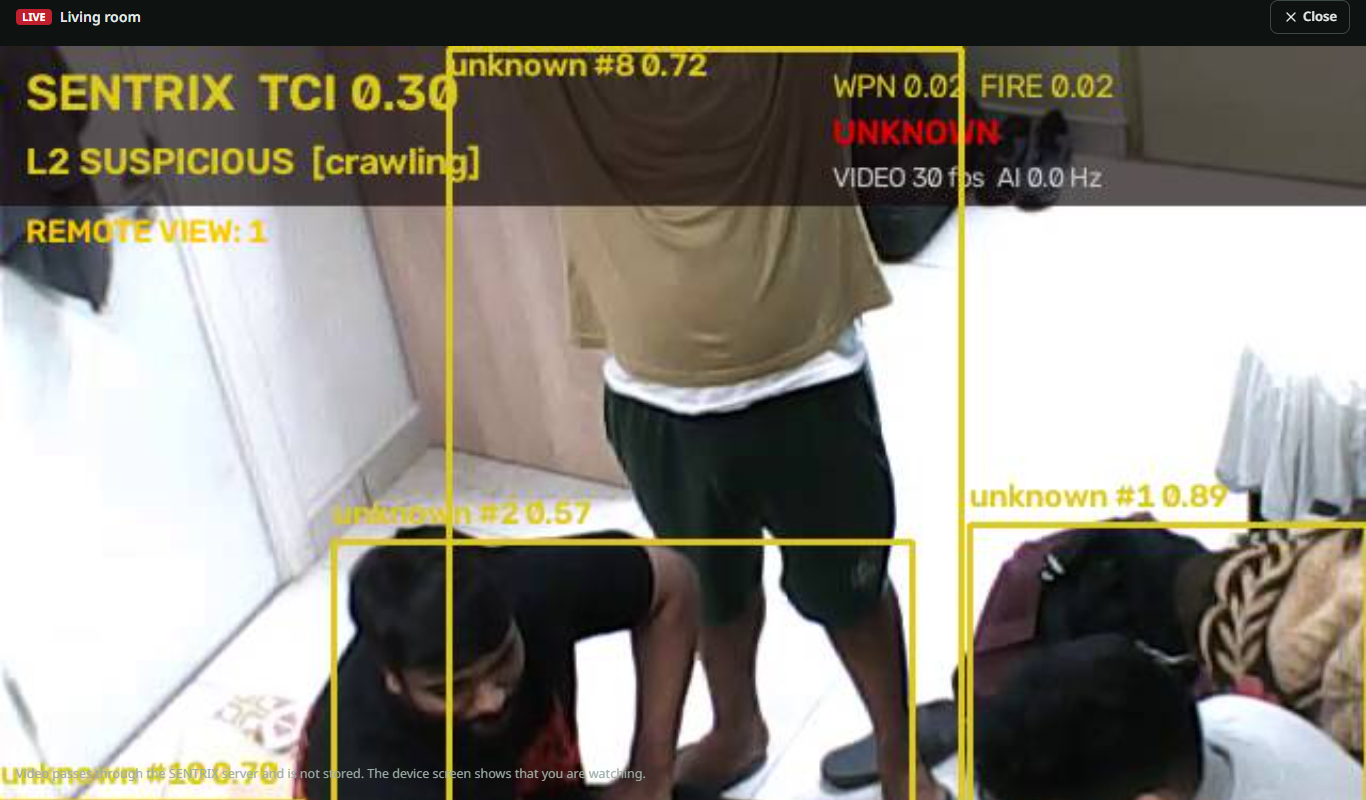
\includegraphics[width=0.49\textwidth]{figures/screens_c/portal_live.png}
\caption{Portal: after approval the owner sees ``The SENTRIX Desk is handling it'' with the timeline (left); live view of the device through the tunnel (right)}
\label{fig:scr-ack}
\end{figure}

\begin{figure}[H]
\centering
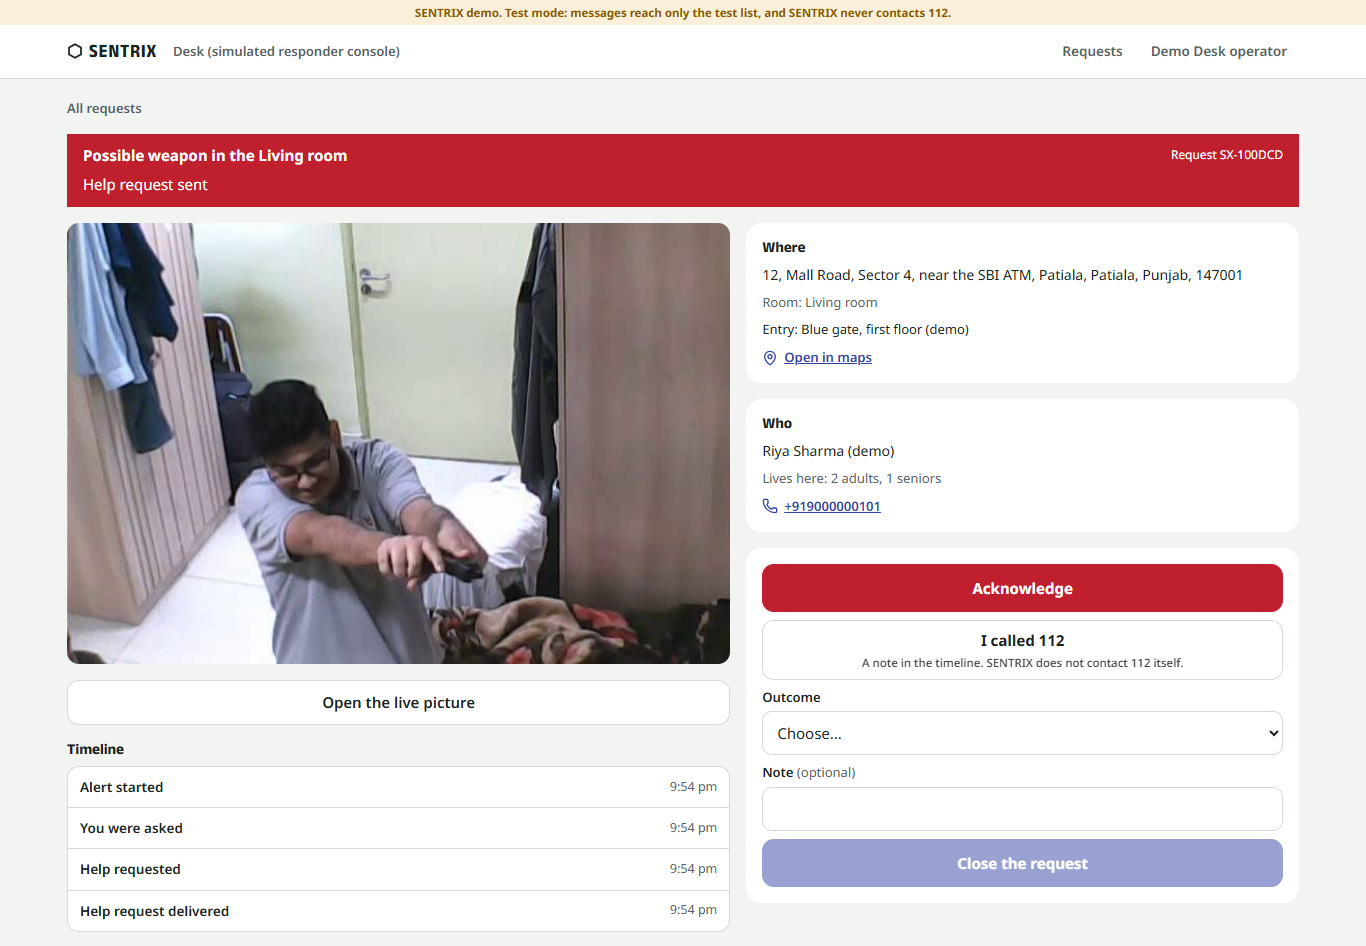
\includegraphics[width=0.66\textwidth]{figures/screens_c/desk_request.png}\hfill
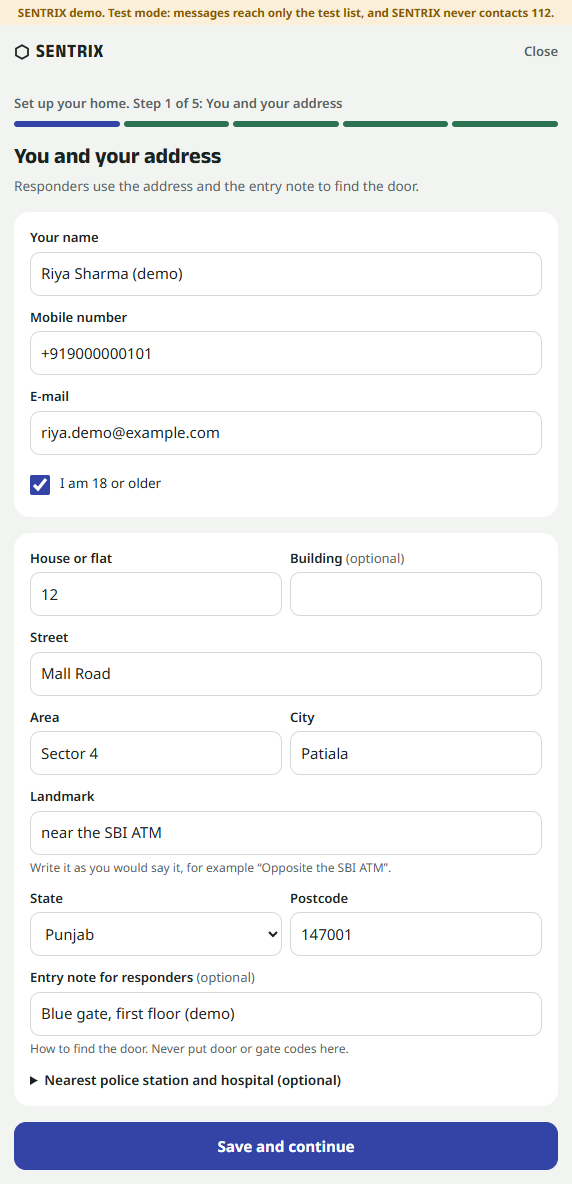
\includegraphics[width=0.32\textwidth]{figures/screens_c/portal_onboarding.png}
\caption{SENTRIX Desk request page with location, household, snapshot, acknowledge and close (left); onboarding wizard, step 1 (right)}
\label{fig:scr-desk}
\end{figure}

\begin{figure}[H]
\centering
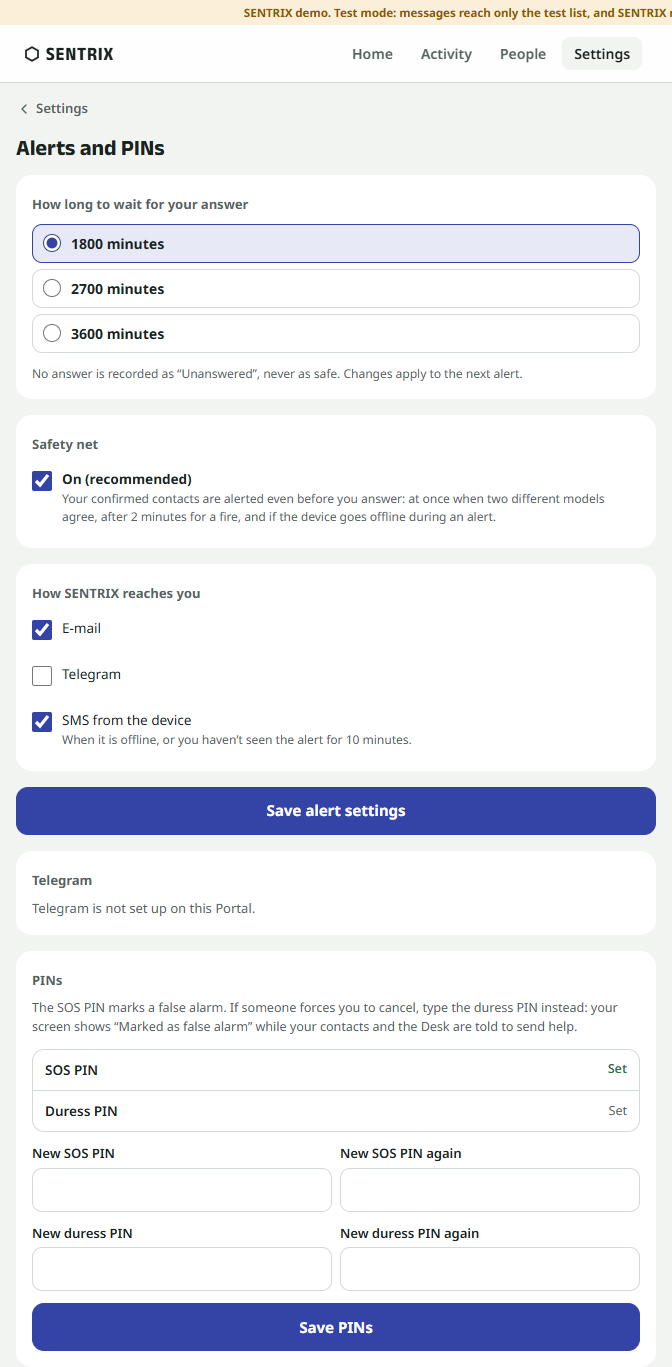
\includegraphics[width=0.32\textwidth]{figures/screens_c/portal_settings_alerts.png}\hfill
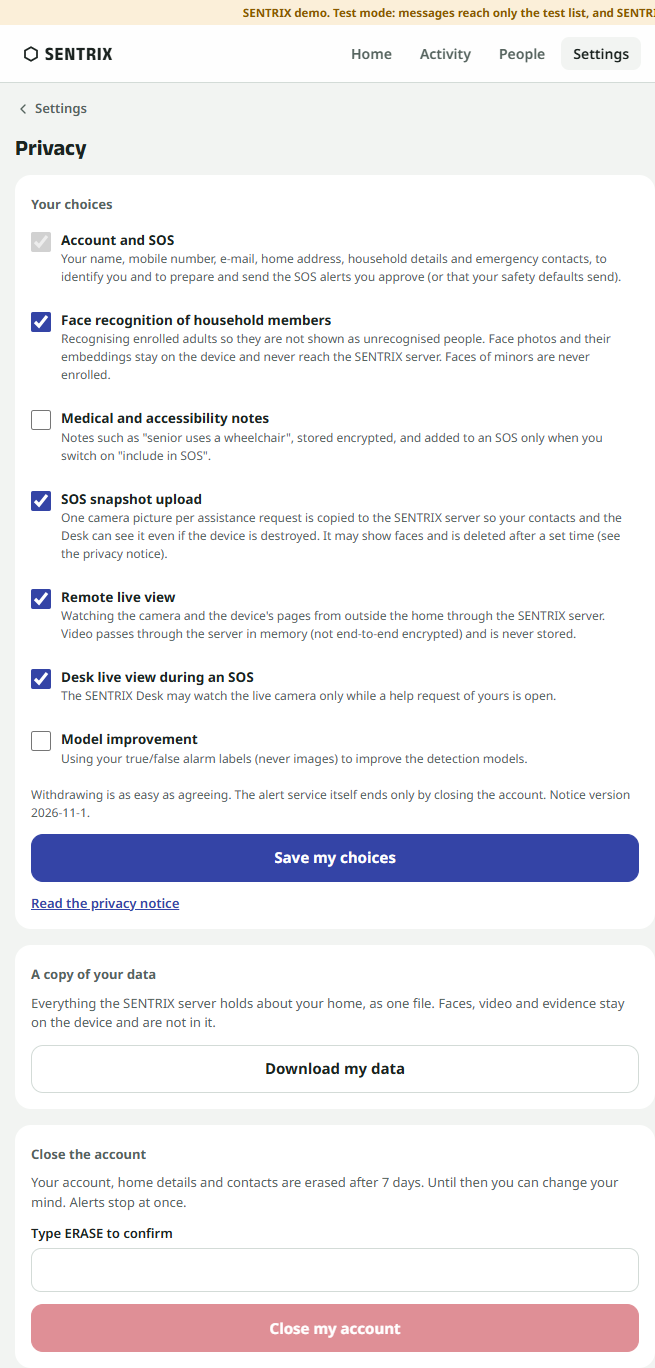
\includegraphics[width=0.32\textwidth]{figures/screens_c/portal_privacy.png}\hfill
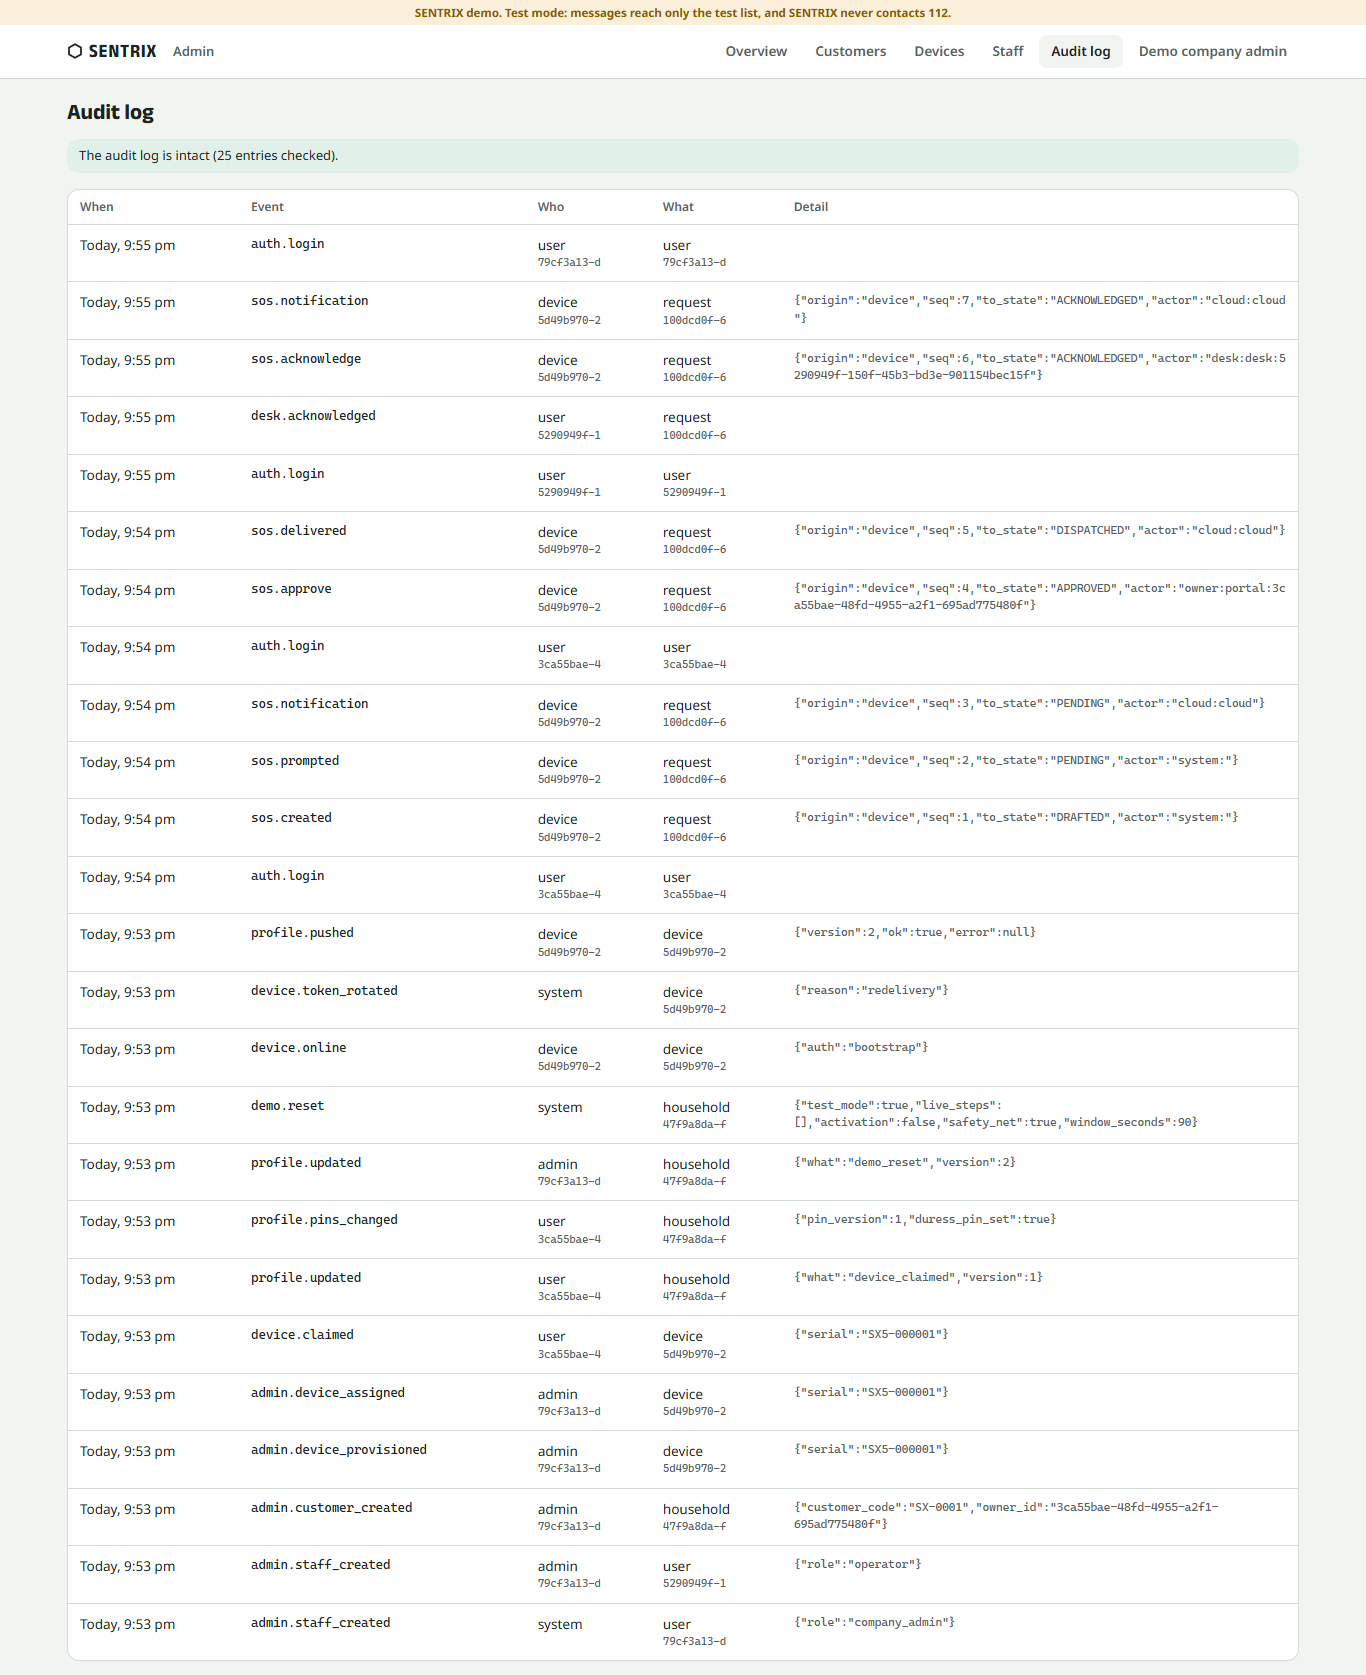
\includegraphics[width=0.32\textwidth]{figures/screens_c/admin_audit.png}
\caption{Portal: alert and PIN settings (left), privacy choices, export and erasure (centre), and the company audit log, whose hash chain is verified (right)}
\label{fig:scr-settings}
\end{figure}

%--------------------------------------------------------------
\section{Testing Process}
\label{sec:testing}

\subsection{Test Plan}
The test plan follows the structure of ISO/IEC/IEEE 29119-3 \cite{iso29119}.
\begin{itemize}
\item \textbf{Objective:} show that every requirement of Section~\ref{sec:srs} is met, that no test can ever send a real alert, and that detection performance is measured the way the product is used.
\item \textbf{Items under test:} the device package, the Portal, the two React applications, the deployment kits and the evaluation tools.
\item \textbf{Environment:} the laptop (Python 3.14, CPU), Microsoft Edge for browser tests; hardware behind fakes (gpiozero mock pins, fake Picamera2, fake \code{vcgencmd} and \code{/sys}, a fake AT-command serial port, fake Telegram/e-mail transports, a fake sound library).
\item \textbf{Isolation:} \code{tests/conftest.py} runs before any import: test mode on, every live switch off, provider keys blanked, the device's \code{var/} tree and the Portal database moved to a temporary directory, webcam and microphone blocked, and a socket guard that allows loopback only.
\item \textbf{Entry criteria:} code builds, the doctor tool passes. \textbf{Exit criteria:} the full suite passes; replay results equal or better than the previous milestone at Level~3 and above; no unexplained regression in benchmarks.
\item \textbf{Schedule:} the suite runs before every commit of a milestone (about 6.5 minutes); replays and benchmarks at every model or rule change.
\end{itemize}

\subsection{Features to be Tested}
Perception wrappers and model loading; evidence confirmation, corroboration, fight and banter rules; TCI and level policy; incidents, event log and evidence vault (including crash safety); per-track identity and body re-identification; audio alignment and the microphone chooser; the clip engine, fast lane and runtimes; the SOS machine, policy, PINs, sweeper and service; channels, outbox and the send guard; the link client, tunnel and path table; the Local Console API and its security (sessions, CSRF, CSP, rate limits); recordings; the Portal's accounts, onboarding, household, contacts, Desk, admin, privacy and retention; Pi hardware services; deployment kits; and the end-to-end product flow.

\subsection{Test Strategy}
Testing is layered (\figref{fig:tests}):
\begin{enumerate}
\item \textbf{Unit tests} for pure logic (the SOS machine, evidence rules, policy, resampler, recorder frame grid).
\item \textbf{Integration tests} for each service with its real neighbours and fake transports (channels with fake Telegram and modem; the link client against the Portal hub over an in-memory pipe).
\item \textbf{In-process product tests:} \code{tests/test\_e2e\_product.py} runs the Portal, the device console with a fake pipeline, the real SOS engine on an injected clock and the real link client in one event loop through 13 scenarios.
\item \textbf{Browser end-to-end tests:} Playwright drives Microsoft Edge against the real Portal and device processes in a fresh test-mode demo world, at desktop and phone sizes.
\item \textbf{Evaluation as regression:} replay of the ten labelled videos and of the recorded live session after every change to rules or models.
\item \textbf{Live smoke runs and reviews:} the Portal and the device as two real processes linked over a real WebSocket, and adversarial reviews in which each finding needs a concrete failing case before it is fixed.
\end{enumerate}

\begin{figure}[htbp]
\centering
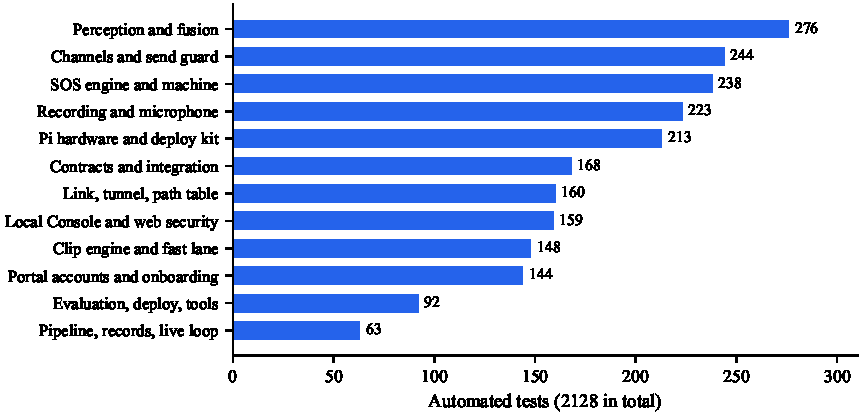
\includegraphics[width=0.85\textwidth]{figures/fig_tests.pdf}
\caption{Automated tests per area (2128 collected on the device and Portal branch)}
\label{fig:tests}
\end{figure}

\subsection{Test Techniques}
\begin{itemize}
\item \textbf{Equivalence partitioning and boundary values:} scores exactly at a threshold, 1 of 3 versus 2 of 3 confirmations, gaps just under and over 3\,s, dwell times of 0.59 and 0.61\,s, recordings at the 2\,GB floor.
\item \textbf{State-transition testing:} every allowed and forbidden transition of the SOS table, duress parity (the owner's screens after a duress PIN must equal a normal false alarm), reconnect merges.
\item \textbf{Time travel:} the SOS engine and the Portal workers run on an injected clock, so 30-minute windows, reminders and safety defaults are tested in milliseconds.
\item \textbf{Fault injection:} 100 forced link disconnects (no event lost), \code{taskkill /F} during an open incident (no event row lost), a real \code{os.\_exit} crash during a recording (the partial files are recovered), a modem that browns out, Telegram returning errors.
\item \textbf{Security tests:} CSRF without a token, cross-household access, XSS in names, the tunnel's path table per role, secrets never in a response, rate limits.
\item \textbf{Replay regression:} the recorded live session re-decided under each new rule set.
\end{itemize}

\subsection{Test Cases}
\tabref{tab:testcases} lists representative test cases; each is an automated test in the repository.

\begin{longtable}{|C{0.95cm}|L{2.9cm}|L{4.3cm}|L{3.4cm}|C{0.95cm}|}
\caption{Representative test cases}\label{tab:testcases}\\
\hline\rowhead
\thead{ID} & \thead{Feature (test file)} & \thead{Input / steps} & \thead{Expected result} & \thead{Result}\\ \hline
\endfirsthead
\hline\rowhead
\thead{ID} & \thead{Feature (test file)} & \thead{Input / steps} & \thead{Expected result} & \thead{Result}\\ \hline
\endhead
\multicolumn{5}{r}{\footnotesize\itshape continued on next page}\\
\endfoot
\endlastfoot
\tablefont TC-01 & \tablefont Confirmation (test\_evidence) & \tablefont One scene vote over threshold, then two below & \tablefont Not confirmed; TCI below Level~2 & \tablefont Pass\\ \hline
\tablefont TC-02 & \tablefont Confirmation (test\_evidence) & \tablefont A cached value carried on later ticks & \tablefont Does not count again; never confirms itself & \tablefont Pass\\ \hline
\tablefont TC-03 & \tablefont Person gate & \tablefont Weapon votes with no person for 2.5\,s & \tablefont Weapon gated, no alarm & \tablefont Pass\\ \hline
\tablefont TC-04 & \tablefont Corroboration (test\_multimodal) & \tablefont Pistol box + gunshot sound aligned & \tablefont Level~4 & \tablefont Pass\\ \hline
\tablefont TC-05 & \tablefont Audio alone & \tablefont Scream with no visual source & \tablefont At most Level~2, never a weapon & \tablefont Pass\\ \hline
\tablefont TC-06 & \tablefont Banter & \tablefont Video fight + aligned laughter & \tablefont Held at Level~2, labelled banter & \tablefont Pass\\ \hline
\tablefont TC-07 & \tablefont Stale audio & \tablefont Audio window 3\,s before the frame & \tablefont Audio ``unavailable'', no vote & \tablefont Pass\\ \hline
\tablefont TC-08 & \tablefont Unknown person & \tablefont Stranger present 10\,s at home & \tablefont Level~2 only, no snapshot, no SOS & \tablefont Pass\\ \hline
\tablefont TC-09 & \tablefont Level policy (test\_fusion) & \tablefont TCI ramp rising across several bands & \tablefont Each level commits as earned; L4/L5 after 0.6\,s and 2 observations & \tablefont Pass\\ \hline
\tablefont TC-10 & \tablefont Records (test\_records) & \tablefont Incident row left open by a crash & \tablefont Every event row on disk before close; open row closed at the next start & \tablefont Pass\\ \hline
\tablefont TC-11 & \tablefont Evidence (test\_clip\_engine) & \tablefont Two clip bundles sealed & \tablefont Manifest hash chain verifies with 2 entries & \tablefont Pass\\ \hline
\tablefont TC-12 & \tablefont Identity (test\_identity) & \tablefont Resident and stranger in view (tailgating) & \tablefont Stranger stays unknown & \tablefont Pass\\ \hline
\tablefont TC-13 & \tablefont Re-id (test\_reid) & \tablefont Armed mode, body matches resident & \tablefont Not authorised (face only) & \tablefont Pass\\ \hline
\tablefont TC-14 & \tablefont SOS machine (test\_sos\_machine) & \tablefont Confirmed weapon L3 & \tablefont One request DRAFTED $\to$ PENDING; later incidents attach & \tablefont Pass\\ \hline
\tablefont TC-15 & \tablefont SOS expiry & \tablefont No answer for the whole window & \tablefont EXPIRED, labelled ``Unanswered'', never ``safe'' & \tablefont Pass\\ \hline
\tablefont TC-16 & \tablefont Duress (test\_sos\_engine) & \tablefont Duress PIN entered & \tablefont Screen shows false alarm; contacts and Desk alerted & \tablefont Pass\\ \hline
\tablefont TC-17 & \tablefont PIN lockout (test\_sos\_pins) & \tablefont Five wrong PINs & \tablefont Answers locked for 10 minutes & \tablefont Pass\\ \hline
\tablefont TC-18 & \tablefont Safety default & \tablefont Fire request unanswered for 2 min & \tablefont Confirmed contacts alerted & \tablefont Pass\\ \hline
\tablefont TC-19 & \tablefont Send guard (test\_ch\_router) & \tablefont Message to 112 with live switches on & \tablefont Always refused & \tablefont Pass\\ \hline
\tablefont TC-20 & \tablefont Test mode & \tablefont Recipient not on the allowlist & \tablefont SUPPRESSED, nothing sent & \tablefont Pass\\ \hline
\tablefont TC-21 & \tablefont Link (test\_integration\_m10) & \tablefont 100 forced disconnects & \tablefont 0 events lost after reconnect & \tablefont Pass\\ \hline
\tablefont TC-22 & \tablefont Path table (test\_link\_policy) & \tablefont Tunnelled request for a LAN-only page or an unknown write & \tablefont Refused & \tablefont Pass\\ \hline
\tablefont TC-23 & \tablefont Isolation (test\_acct\_isolation) & \tablefont Owner A requests household B's data & \tablefont 403/404, nothing leaked & \tablefont Pass\\ \hline
\tablefont TC-24 & \tablefont Siren (test\_hw\_siren) & \tablefont Activation of 120\,s & \tablefont Released after at most 90\,s & \tablefont Pass\\ \hline
\tablefont TC-25 & \tablefont Recorder (test\_recorder) & \tablefont Crash by \code{os.\_exit} while recording & \tablefont Partial files recovered at next start & \tablefont Pass\\ \hline
\tablefont TC-26 & \tablefont Product flow (test\_e2e\_product) & \tablefont Provision $\to$ activate $\to$ onboard $\to$ claim $\to$ L3 $\to$ approve $\to$ Desk & \tablefont Request CLOSED, verdict TRUE & \tablefont Pass\\ \hline
\tablefont TC-27 & \tablefont Browser: alert journey (sos.spec) & \tablefont Scripted weapon; owner answers; Desk acknowledges and closes & \tablefont Every screen updates; no \code{tel:112} link in test mode & \tablefont Pass\\ \hline
\tablefont TC-28 & \tablefont Browser: false alarm on a phone & \tablefont Wrong PIN, then the right PIN & \tablefont Wrong PIN refused; marked as false alarm & \tablefont Pass\\ \hline
\tablefont TC-29 & \tablefont Browser: add a contact (owner.spec) & \tablefont Owner adds an emergency contact & \tablefont Confirmation step with a one-time link shown & \tablefont \textbf{Fail}\\ \hline
\end{longtable}

\subsection{Test Results}
\label{sec:test-results}
\begin{itemize}
\item \textbf{Device and Portal suite} (branch \code{sentrix/portal}, commit \code{5127b3c}, with body re-identification, the v5 detector heads and room calibration): \textbf{2154 passed} in 386.6\,s on the laptop. The device guard blocked 4 webcam/microphone attempts and the socket guard 2 network attempts---all made deliberately by the tests that check those guards.
\item \textbf{Frontend branch} (\code{sentrix/frontend-v2}, commit \code{c1241c1}, the React applications): Python suite \textbf{2243 passed, 1 skipped} in 385.4\,s; Vitest unit tests \textbf{15 of 15} passed; Playwright browser tests \textbf{22 of 23} passed at desktop and phone sizes. The failing case (TC-29) is the owner adding an emergency contact: the page did not show the ``ask the contact to confirm'' step within 15\,s. It is a known defect to be fixed before the final demonstration; adding contacts through onboarding is covered by passing tests.
\item \textbf{Live smoke run} (Portal and device as two real processes linked over a real WebSocket, demo reel): every Local Console page and 14 GET APIs gave the same status directly and through the tunnel; ``scene gun'' produced a PENDING weapon request 8.0--9.8\,s after the clip started and ``scene fire'' 11.6--11.9\,s; approval reached the device as DISPATCHED in 0.01--0.28\,s; MJPEG ran at 29.9\,fps directly and 13.6\,fps through the tunnel (cap 15). Five defects found in the run were fixed with regression tests.
\item \textbf{Live on the Raspberry~Pi~5 with the Render Portal and Telegram:} detections in the demo room opened assistance requests that were prompted on the Pi's screen and the owner's phone; requests were declined with the PIN, expired unanswered, and in one case approved, dispatched and resolved on the Desk. These were false alarms from the scene classifier in the new room, and they are the data from which the room thresholds were set (Section~\ref{sec:results}).
\item \textbf{Bug sweep and audits:} a five-way code audit and a twelve-item bug sweep (October 2026) and a wiring and copy audit (November 2026) each fixed every confirmed finding with a regression test.
\end{itemize}

%--------------------------------------------------------------
\section{Results and Discussions}
\label{sec:results}

\subsection{Choosing the models}
\figref{fig:configs} compares the three model configurations on the held-out validation videos and on the replay of all ten videos. The models trained on the team's own footage (v4: DINOv2 scene classifier and YOLO11n heads) nearly doubled validation macro-F1 over the fine-tuned v3 models (0.768 vs 0.401) and cut false alarms per normal minute by a factor of nine (0.79 vs 7.12); the evidence rules of M1 then removed the remaining false alarms (0.00) while keeping the same 13 of 18 episodes. The one clear loss of v4 is the test corridor's swung stick, which it never detects (0 of 3 episodes): 39 frames of a stick \emph{carried} in one training video did not teach a stick \emph{swung} in another. Stick is therefore experimental in the product.

\begin{figure}[htbp]
\centering
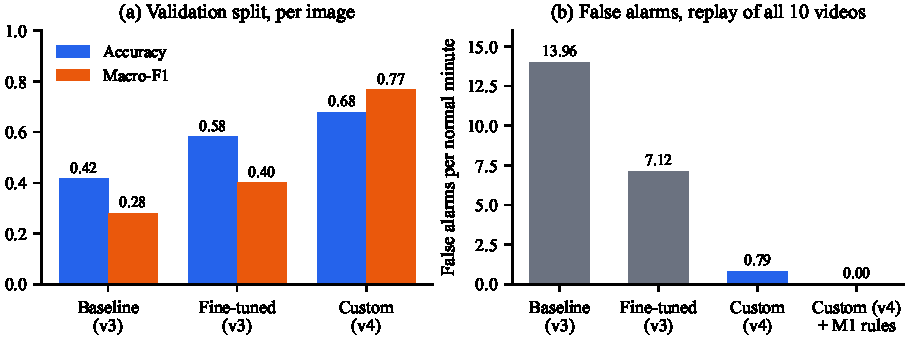
\includegraphics[width=\textwidth]{figures/fig_configs.pdf}
\caption{Model configurations on the custom dataset: (a) validation accuracy and macro-F1 per image; (b) false alarms per minute of normal footage in the replay of all ten videos}
\label{fig:configs}
\end{figure}

\begin{table}[htbp]
\caption{Held-out results of the three configurations (validation: gun, vid04; test: wa02)}
\label{tab:configs}
\centering\tablefont
\begin{tabularx}{\textwidth}{|Y|C{2.6cm}|C{2.6cm}|C{2.6cm}|}
\hline\rowhead
\thead{Measure} & \thead{Baseline (v3)} & \thead{Fine-tuned (v3)} & \thead{Custom (v4)}\\ \hline
Validation per image: accuracy / macro-F1 & 0.417 / 0.281 & 0.583 / 0.401 & \textbf{0.679 / 0.768}\\ \hline
Validation replay: episodes / false alarms & 1 of 2 / 0 & 1 of 2 / 4 & \textbf{2 of 2 / 0}\\ \hline
Test per image: accuracy / macro-F1 & 0.043 / 0.114 & 0.677 / \textbf{0.460} & \textbf{0.720} / 0.419\\ \hline
Test replay: stick episodes & 3 of 3 (alarms on everything) & \textbf{3 of 3} & 0 of 3\\ \hline
False alarms per normal minute, all 10 videos & 13.96 & 7.12 & \textbf{0.79}\\ \hline
Leave-one-video-out macro-F1 of the scene model & -- & 0.210 & \textbf{0.440}\\ \hline
\end{tabularx}
\end{table}

\subsection{Effect of the evidence rules}
\figref{fig:livesession} re-decides the first live session under the rules of each stage. As logged, the old pipeline committed 30 onsets at Level~2 and above, 9 at Level~3 and 6 at Level~4 in 18.3 minutes. Under the M1 rules the same log gives 0, 0 and 0. Under the final rules (D15) it gives 5 Level~2 onsets---the by-design ``someone we don't recognise'' notices for unenrolled team members---and still 0 at Level~3 and above. The cost was latency: on the held-out handgun video the first Level~3 came 6.3\,s after the episode began instead of 2.4\,s, because the scene probability stays under the raised 0.50 floor for the first seconds.

\begin{figure}[htbp]
\centering
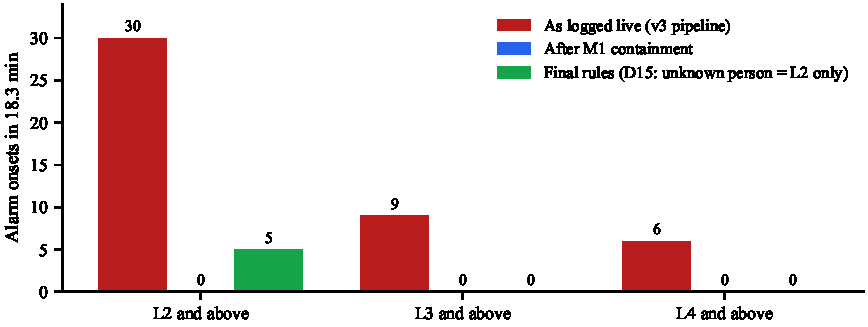
\includegraphics[width=0.92\textwidth]{figures/fig_live_session.pdf}
\caption{The first live session (18.3 minutes, laptop webcam) re-decided under each rule set}
\label{fig:livesession}
\end{figure}

\subsection{Detection per committed level}
\figref{fig:levels} and \tabref{tab:levels-res} show what reaches each level when the ten videos are replayed through the final pipeline with their own soundtracks. Three quarters of the handgun episodes and all flame episodes reach Level~3 (assistance request); half the handgun episodes and two of three flames are corroborated to Level~4; two handgun episodes and two flames reach Level~5 (siren). No normal footage produced an onset at Level~3 or above. The staged fights (vid05) do not reach Level~3: their soundtrack sounds like calm talk (benign 0.91, aggression below 0.01), so the fight rule correctly withholds the corroboration it needs.

\begin{figure}[htbp]
\centering
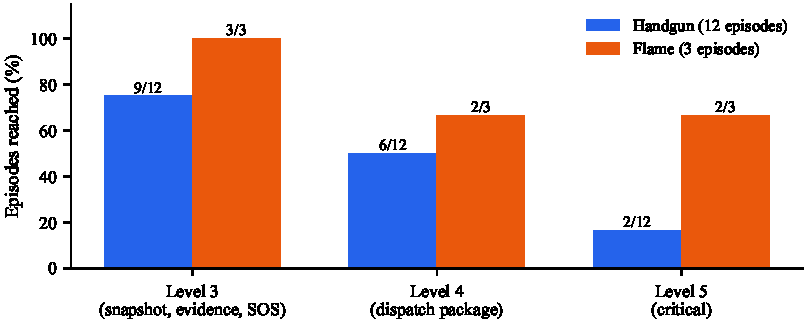
\includegraphics[width=0.85\textwidth]{figures/fig_levels.pdf}
\caption{Episodes reaching each committed level in the replay of the ten videos (tick mode, time-aligned soundtracks)}
\label{fig:levels}
\end{figure}

\begin{table}[htbp]
\caption{Committed-level results (all ten videos, partly in-sample)}
\label{tab:levels-res}
\centering\tablefont
\begin{tabularx}{\textwidth}{|Y|C{2.2cm}|C{2.2cm}|C{2.6cm}|}
\hline\rowhead
\thead{Measure} & \thead{Tick mode, 6\,Hz} & \thead{Tick mode, 2\,Hz} & \thead{Clip mode + fast lane}\\ \hline
Handgun at Level 3 / 4 / 5 & 9/12, 6/12, 2/12 & 9/12 at L3 & 9/12, 6/12, 5/12\\ \hline
Flame at Level 3 / 4 / 5 & 3/3, 2/3, 2/3 & 3/3 at L3 & 3/3, --, 2/3\\ \hline
Robbery / assault at Level 3 & 0/1 / 0/2 & 0/1 / 0/2 & 0/1 / 0/2\\ \hline
False onsets at Level 3 and above (3.7 normal minutes) & 0 & 0 & 0\\ \hline
Upper 95\,\% bound on false Level~3 onsets & 60 per hour & 60 per hour & 60 per hour\\ \hline
Frame AUROC of the scene model, weapon / fire & 0.93 / 0.999 & -- & --\\ \hline
\end{tabularx}
\end{table}

These numbers are encouraging but not a validation: seven of the ten videos were used in training, and 3.7 minutes of normal footage can only bound the false-alarm rate at 60 per hour, far above what a home needs. Two release gates measured on this data fail: G2 (handgun episodes confirmed within 2\,s: 8 of 12) and G4 (onset to Level~3 at the 95th percentile: 4.0\,s against 2\,s).

\subsection{Detector heads retrained on fifteen videos}
The weapon and fire heads were retrained from the v4 heads on all 977 frames (fifteen videos, 180 boxes) with 2000 public images mixed back in, so that the public classes are not forgotten. The weapon head gained knife and long-gun classes. Each head had to pass bars fixed before training:
\begin{itemize}
\item no rise in false alarms on the held-out normal frames of the validation and test videos;
\item validation weapon AUROC not lower by more than 0.02 (fire: not lower);
\item public pistol (fire) AP50 not lower.
\end{itemize}
Both passed (\tabref{tab:v5heads}). On the held-out validation videos the weapon head's frame AUROC rose from 0.748 to 0.871 and the fire head's from 0.587 to 0.964, with no new false alarms. On the public test sets, which the v4 heads had forgotten, pistol AP50 went from 0.007 to 0.699, and the new knife class reached 0.717.

In the replay of all fifteen videos, 11 of 14 weapon episodes reach Level~3 instead of 9: the new handgun and knife scenes now raise an assistance request. The false Level~3 onset count is unchanged at 1 in 4.9 minutes of normal footage. Two results did not improve:
\begin{itemize}
\item the two flames that reached Level~5 now stop at Level~4;
\item the small aerosol flame of \code{vid04} still scores below the fire head's vote.
\end{itemize}
The five new videos are in the training split, so their replay is in-sample.

The scene classifier was not retrained in this step. Measured on the five new videos it recognises the new scenes poorly: accuracy 0.43, macro-F1 0.16, 1 of 47 weapon frames. It raised no false weapon or fire alarm on their 90 normal frames.

\begin{table}[htbp]
\caption{v4 and v5 detector heads (held-out validation: gun, vid04; replay: all fifteen videos, tick mode at 6\,Hz with their soundtracks, partly in-sample)}
\label{tab:v5heads}
\centering\tablefont
\begin{tabularx}{\textwidth}{|Y|C{3.0cm}|C{3.0cm}|}
\hline\rowhead
\thead{Measure} & \thead{v4 heads} & \thead{v5 heads}\\ \hline
Validation frame AUROC, weapon / fire & 0.748 / 0.587 & \textbf{0.871 / 0.964}\\ \hline
False alarms on held-out normal frames at 0.25 (validation / test), weapon & 0.000 / 0.015 & 0.000 / 0.015\\ \hline
Public test AP50: pistol / knife / fire & 0.007 / -- / 0.000 & \textbf{0.699 / 0.717 / 0.487}\\ \hline
Weapon episodes at Level 3 / 4 / 5 & 9/14, 6/14, 2/14 & \textbf{11/14}, 6/14, 2/14\\ \hline
Flame episodes at Level 3 / 4 / 5 & 3/3, 2/3, 2/3 & 3/3, 2/3, 0/3\\ \hline
False onsets at Level 3 (4.9 normal minutes) & 1 & 1\\ \hline
\end{tabularx}
\end{table}

\subsection{Real-time performance}
\figref{fig:liveloop} shows the live loop on the laptop before and after the M2 repair, measured with \code{tools/bench\_live.py} on a video with four faces. Separating capture, inference and preview, turning off the ONNX Runtime spin-wait and moving face recognition to its own thread raised the preview from 0.6 to 29.7\,fps and the AI rate from 0.32 to 5.6 decisions per second (tick p50 168\,ms, frame age p50 198\,ms).

\begin{figure}[htbp]
\centering
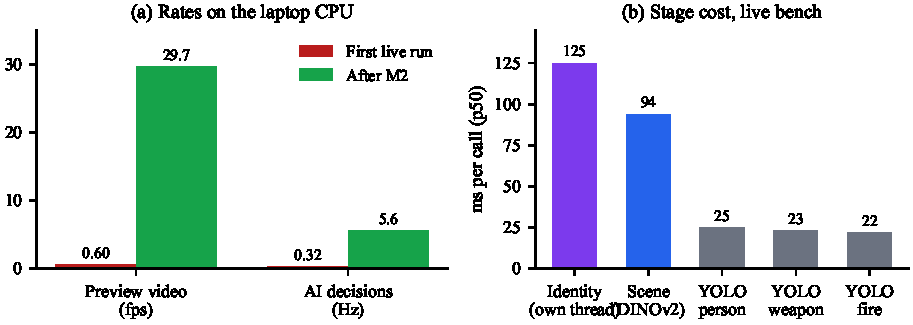
\includegraphics[width=\textwidth]{figures/fig_live_loop.pdf}
\caption{Live loop on the laptop CPU: (a) preview and AI rates before and after M2; (b) cost of each stage}
\label{fig:liveloop}
\end{figure}

On the Raspberry~Pi~5 the same models must share four cores. \figref{fig:piclip} shows the clip engine measured on the Pi with the held-out handgun clip as a 30\,fps camera. At 640\,px the object stage alone takes 5.6\,s and three clips in four are dropped; at 320\,px the clip takes 3.9\,s, every other clip is analysed and decisions are about 4\,s old, with the same Level~3 recall on the replay (9/9 handgun, 3/3 fire on the nine training and validation videos) and one Level~4 handgun episode fewer. The shipped profile is therefore 320\,px with two scene frames; the fast lane (about 3.5 passes per second, 35--39\,ms per head at 320\,px) provides the quick Level~3 path. The 1.6\,s budget is not yet met: the DINOv2 stage alone takes about 1.2\,s per frame on the Pi, which is why a Hailo NPU or an NCNN build is the planned next step.

\begin{figure}[htbp]
\centering
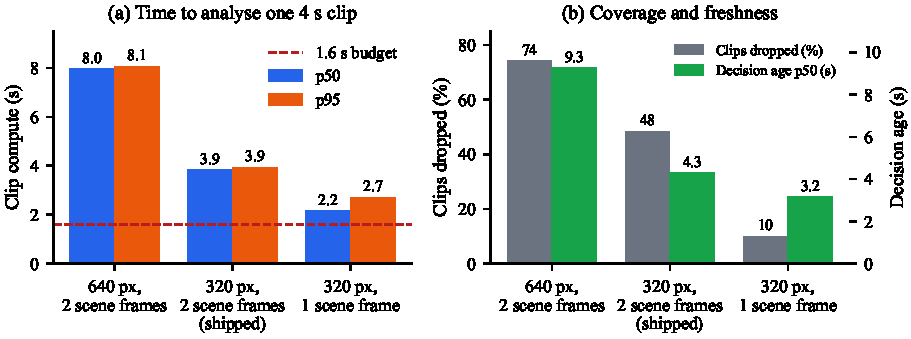
\includegraphics[width=\textwidth]{figures/fig_pi_clip.pdf}
\caption{Clip engine on the Raspberry~Pi~5: (a) time to analyse one 4\,s clip; (b) share of clips dropped and age of decisions}
\label{fig:piclip}
\end{figure}

\subsection{Slim models for the Pi (a rejected hypothesis)}
To make the scene stage fit the Pi, MobileNetV3-L and EfficientNet-B0 heads were trained under a protocol fixed in advance (\figref{fig:slim}). They are 25--40 times faster (2.4 and 4.3\,ms in ONNX Runtime) but reach LOVO macro-F1 of only 0.229 and 0.211 against 0.440 for DINOv2, below the pre-registered bar of 0.396, and neither recognises fire in a video it has not seen. Distillation from DINOv2 did not help (0.211--0.224): the cross-video generalisation of DINOv2 lies in its self-supervised features, which an ImageNet CNN does not have. DINOv2 stayed in the product.

\begin{figure}[htbp]
\centering
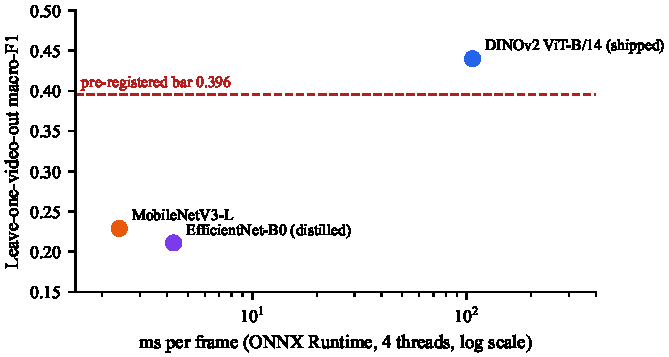
\includegraphics[width=0.72\textwidth]{figures/fig_slim.pdf}
\caption{Accuracy against speed of the scene classifiers (leave-one-video-out)}
\label{fig:slim}
\end{figure}

\subsection{Body re-identification}
\figref{fig:reid} shows the evaluation of body matching on ByteTrack tracks of the nine training and validation videos (4524 same-person pairs, 2498 different-people pairs).
\begin{itemize}
\item \textbf{Same weights as the prototype.} The earlier IntrusionSentry prototype used OSNet x1\_0 with ImageNet weights. These separate people better than colour histograms (AUROC 0.83 against 0.73).
\item \textbf{Re-identification-trained weights.} OSNet x1\_0 and OSNet-AIN x1\_0, both trained for re-identification on MSMT17, do better still (0.92 and 0.93). OSNet-AIN was chosen by a rule fixed before the comparison: the most same-person cases at a bar that accepts at most 0.05\,\% of different people.
\item \textbf{Speed.} These checkpoints contain denormal weights, which made CPU inference 6--17 times slower. Zeroing them brought OSNet-AIN to 10.3\,ms per crop with unchanged features.
\end{itemize}
With the five November videos (fourteen videos; 1500 same-person and 25,408 different-people cases of the identity rule), the bar moved from 0.86 to 0.87. The rule, 20 looks and two checks in a row, reaches AUROC 0.97 and accepts 30\,\% of same-person cases and 0.020\,\% of different people.

The prototype's cosine bar of 0.50 would have accepted 97.2\,\% of different people on the ImageNet features and 50\,\% on the shipped ones. At SENTRIX's bar a wrong match is rare, and it can at most hide a Level~2 notice at home.

\begin{figure}[htbp]
\centering
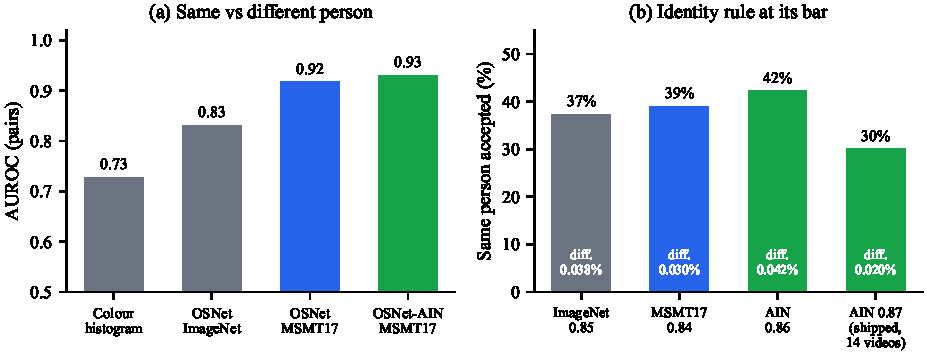
\includegraphics[width=\textwidth]{figures/fig_reid.pdf}
\caption{Body re-identification: (a) separation of same and different people with four body models (nine videos); (b) the identity rule at each model's bar, and the shipped OSNet-AIN bar on fourteen videos}
\label{fig:reid}
\end{figure}

\subsection{Calibration in the demonstration room}
In about ten hours after the Pi was installed in the demo room, the scene classifier alone raised 16 weapon Level~3 alarms (the weapon detector confirmed none), and later two fire Level~3 alarms, with no weapon or flame present. The Pi's own logs (8077 clips for weapon, 5435 scored clips for fire) show why (\figref{fig:room}): in this room the classifier's p(weapon) has a median of 0.19 but a 99.9th percentile of 0.65 and a maximum of 0.742, above the 0.50 floor; p(fire) peaks at 0.646 against a 0.45 floor. Per-room thresholds of 0.75 (weapon) and 0.70 (fire) remove every one of these false alarms. The cost is stated openly: a small flame that the classifier scores below 0.70 (the held-out vid04 peaks at 0.636 in clip mode) no longer reaches Level~3 from the classifier alone and needs the fire detector; the replica-gun and replica-flame tests in that room are part of the remaining work.

\paragraph{Calibration from the device's own log.} Setting those thresholds meant reading the Pi's log by hand, and every new room or new model would need it again. A tool now does it by a rule fixed in advance (\code{tools/calibrate\_room.py}, decision D23). It reads the device's own event log for a period the team asserts was quiet, and replays the device's confirmation rule at every possible threshold. On the Pi that rule is two keyframes per clip, with a weapon keyframe counting only if a person was seen in the last 2\,s; the replay rebuilds that gate from the logged person boxes. It then proposes
\begin{equation}
\theta_c = \max\big(\text{floor}_c,\ \hat{c}_c + 0.10,\ \hat{s}_c + 0.01\big),
\label{eq:calib}
\end{equation}
rounded up to 0.01, where $\hat{c}_c$ is the highest value at which a quiet clip would still have been confirmed and $\hat{s}_c$ the highest single score. The tool also checks itself: wherever the device logged its own decision, the replay at the device's threshold must reach the same one.

On the Pi it was run over SSH and read the logs without changing anything on the device. \tabref{tab:calib} shows the results:
\begin{itemize}
\item \textbf{Check:} the replay matched the device's own decision on all 8,956 logged clips.
\item \textbf{Hand thresholds reproduced:} on the data each hand threshold was set from, the rule gives weapon 0.76 (hand: 0.75) and fire 0.69 (hand: 0.70).
\item \textbf{Whole log:} from 23 October to 19 November the scene model scored 9,092 clips (5.1\,h). The thresholds in force gave no confirmation at all, against 45 weapon and 4 fire onsets at the floors. The 95\,\% upper bound is 0.59 false onsets per hour.
\end{itemize}

The margins were thinner than the rule asks for. One keyframe reached p(weapon) 0.760, above the 0.75 threshold, and a fire confirmation reached 0.650, 0.05 under it. On 19 November the owner therefore approved the proposal, weapon 0.78 and fire 0.75, and it is now in force on the Pi (\figref{fig:room}).

The calibration file records the scene model it was made for. If another model loads, the device keeps the thresholds but flags them as stale, so a retrained model is followed by a new calibration.

The cost is the same as before, one step higher: a replica gun or flame scored between the old and new thresholds no longer reaches Level~3 from the scene model alone. The replica tests in that room, which the tool can replay with \code{--check}, are still to do.

\begin{table}[htbp]
\caption{Room calibration of the demonstration Pi from its own log (clip mode, v4 scene model)}
\label{tab:calib}
\centering\tablefont
\begin{tabularx}{\textwidth}{|Y|C{3.2cm}|C{3.2cm}|}
\hline\rowhead
\thead{Measure} & \thead{Weapon} & \thead{Fire}\\ \hline
Data each hand threshold was set from: scored time & 1.96\,h & 2.40\,h\\ \hline
\quad highest single score / confirming value & 0.742 / 0.590 & 0.646 / 0.587\\ \hline
\quad threshold set by hand / by \eqnref{eq:calib} & 0.75 / 0.76 & 0.70 / 0.69\\ \hline
Whole log (23 Oct -- 19 Nov, 5.1\,h scored): median / p99 / max score & 0.190 / 0.546 / 0.760 & 0.079 / 0.236 / 0.716\\ \hline
\quad onsets at the floor / at the hand threshold & 45 at 0.50 / 0 at 0.75 & 4 at 0.45 / 0 at 0.70\\ \hline
\quad proposed and in force since 19 Nov & \textbf{0.78} & \textbf{0.75}\\ \hline
Replay agrees with the device's own decision & \multicolumn{2}{c|}{8,956 of 8,956 clips}\\ \hline
\end{tabularx}
\end{table}

\begin{figure}[htbp]
\centering
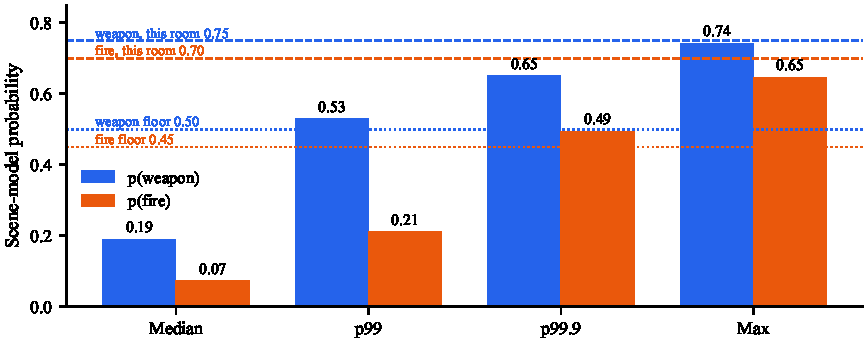
\includegraphics[width=0.92\textwidth]{figures/fig_room_scores.pdf}
\caption{Scene-classifier probabilities in the demo room with no threat present (whole log, 5.1\,h scored), with the default floors and the calibrated room thresholds}
\label{fig:room}
\end{figure}

\subsection{Comparison with related work}
\tabref{tab:sota} compares SENTRIX's components and system-level behaviour with published work. Component scores are not directly comparable---the published numbers come from large public benchmarks and SENTRIX's from two rooms---so the table is read for what each approach measures and where SENTRIX differs.

\begin{table}[htbp]
\caption{Comparison with related state-of-the-art work}
\label{tab:sota}
\centering\tablefont
\begin{tabularx}{\textwidth}{|L{2.4cm}|Y|Y|}
\hline\rowhead
\thead{Aspect} & \thead{Published work} & \thead{SENTRIX}\\ \hline
Handgun alarm & Faster R-CNN alarm after five successive detections fired correctly in 27 of 30 test scenes \cite{olmos2018handgun} & YOLO11n + DINOv2 with 2-of-3 confirmation and a person gate: 9 of 12 episodes at Level~3, 0 false onsets in 3.7 normal minutes (11 of 14 on fifteen videos with the v5 heads); room thresholds calibrated from the device's own logs\\ \hline
Violence & Flow-gated 3D-CNN: 87.25\,\% test accuracy on RWF-2000 \cite{cheng2021rwf}; audio-visual fusion improves XD-Violence \cite{wu2020xdviolence} & ResNet-18 on RWF-2000: 0.832 macro-F1 on a contaminated split; in the product a fight needs video \emph{and} aligned aggression audio, with a banter rule\\ \hline
Audio tagging & PANNs: best model 0.439 mAP on AudioSet \cite{kong2020panns} & PANNs CNN10 at 40\,ms per 4\,s window on a CPU, 527 labels mapped to 7 cues, votes only when time-aligned\\ \hline
Re-identification & OSNet: state of the art on six re-ID datasets with re-ID training \cite{zhou2019osnet} & OSNet-AIN trained on MSMT17 tied to an access decision: AUROC 0.97, 0.020\,\% false accepts at the shipped bar (fourteen videos)\\ \hline
Evaluation & Frame accuracy, mAP or AUROC on curated test sets & Committed-level episodes, false onsets per hour with exact Poisson bounds, onset latency; pre-registered model selection\\ \hline
Alert flow & Detection only, or direct alerting & Owner-approved request, PIN-protected false alarms, duress PIN, safety defaults, ``unanswered'' never ``safe''\\ \hline
Deployment & GPU servers or cloud analysis \cite{shi2016edge} & All inference on a Raspberry~Pi~5; video, faces and evidence stay at home\\ \hline
Recent detectors (2024--2026) & NMS-free YOLOv10s and YOLO26s: 125--130\,ms per frame on a Jetson Nano \cite{fierrosilva2026yolo26weapon}; a review of 101 weapon papers finds little real-world validation \cite{murugan2025weaponreview} & YOLO11n heads at 320\,px take 35--39\,ms per head on the Pi~5 CPU and are judged by committed level in real rooms; YOLO26 is next\\ \hline
VLM and LLM anomaly detection & VadCLIP: 84.51\,\% AP on XD-Violence \cite{wu2024vadclip}; LAVAD: 80.28\,\% AUC on UCF-Crime without training \cite{zanella2024lavad}; MLLMs still limited on smart-home video \cite{zhao2025smarthomebench} & Supervised detectors and published rules on the device; no model's verdict replaces the owner's\\ \hline
Audio-visual fusion (2025) & Align-then-fuse: 86.07\,\% AP on XD-Violence \cite{jin2025aligning} & Time-stamped windows vote only when aligned; banter holds a fight at Level~2\\ \hline
Industry practice & Cloud face recognition in doorbells (2025) \cite{perez2025ringfaces}; police dispatch only with audio, video or witness evidence (2024) \cite{seattle2024alarm} & Faces stay on the device; every request carries a snapshot and a timeline\\ \hline
\end{tabularx}
\end{table}

\section{Inferences Drawn}
\begin{enumerate}
\item \textbf{The decision rules matter more than any single model.} The same models produced 9 Level~3 onsets in 18 minutes or none, depending only on confirmation and corroboration rules.
\item \textbf{Training on one's own footage beats bigger public datasets.} A self-supervised backbone fine-tuned on 765 frames of the target setting outperformed models trained on thousands of public images on every held-out measure except the one class (stick) that the custom data barely contained.
\item \textbf{A new room is a new distribution.} Thresholds valid on the training rooms produced false alarms in the demo room until the room's own logs set them; per-room calibration (now a tool that replays the device's own rule) and deployment-room recordings are part of installing the product, not an afterthought.
\item \textbf{Measuring what the user experiences changes the conclusions.} Per-frame accuracy looked acceptable while the product was unusable; committed-level metrics with confidence bounds showed both the progress and how little normal footage had been seen.
\item \textbf{The Pi can run the whole product, but not yet within the latency target.} With the clip engine and ONNX it analyses every other clip and decides within about 4\,s; the transformer backbone is the bottleneck.
\item \textbf{Safety must be designed into the alert flow.} Silence is not safety, a PIN prevents an intruder from cancelling, and a duress path protects a coerced owner; all of these are testable logic, and the tests found real defects.
\end{enumerate}

\section{Validation of Objectives}
\label{sec:validation}

\begin{table}[H]
\caption{Validation of the approved objectives}
\label{tab:validation}
\centering\tablefont
\begin{tabularx}{\textwidth}{|L{2.4cm}|Y|L{1.6cm}|}
\hline\rowhead
\thead{Objective} & \thead{What was built and the evidence} & \thead{Status}\\ \hline
O1 Multimodal AI pipeline & Weapon (handgun, knife, long gun) and fire detection (YOLO11n), scene and fight classification (DINOv2), faces (InsightFace), bodies (OSNet-AIN), sound (PANNs CNN10), in tick and clip pipelines; handgun 9/12 and flame 3/3 at Level~3 on replay (weapon 11/14 on fifteen videos); 29.7\,fps preview and 5.6\,Hz AI on a laptop; 3.9\,s per clip on the Pi & Achieved; Pi latency target open\\ \hline
O2 Fusion into a TCI & The learned XGBoost fusion of the mid-semester version was retired: it had been fitted to synthetic labels with the meaning of identity inverted and ranked threats worse than its own inputs. It was replaced by transparent, time-aligned evidence rules that produce the same 0--1 TCI and five levels, with every decision re-derivable from the log; live false onsets at Level~3+ fell from 9 to 0 & Achieved with a changed method\\ \hline
O3 Tamper-evident evidence & AES-256-GCM bundles with HKDF keys, SHA-256 digests and an HMAC-signed hash-chained manifest; pre-roll clips in clip mode; a verifier checks every digest and the signed chain & Achieved\\ \hline
O4 Physical edge unit & Raspberry~Pi~5 unit with Camera Module 3, USB microphone, PIR, door and mains inputs, LEDs and a siren relay; bill of materials about Rs.\,40,500 including tools; parametric enclosure; running in the demo room as a systemd service. The ESP32 and DHT22 design of the proposal was replaced by the Pi~5 for camera and audio quality & Achieved (budget revised)\\ \hline
O5 Command console and alerting & React device screen and administration pages, React Portal with onboarding, live view through the tunnel, owner-approved SOS over Portal, device screen, Telegram, e-mail and SMS, the SENTRIX Desk and the admin console; 22 of 23 browser tests pass & Achieved; one UI defect open\\ \hline
\end{tabularx}
\end{table}

%==============================================================
\chapter{CONCLUSIONS AND FUTURE DIRECTIONS}
\label{ch:conclusions}
%==============================================================

\section{Conclusions}
SENTRIX set out to build a home security product that recognises a handgun, a visible flame or a violent fight at the edge, keeps false alarms near zero, puts the owner in control of who is alerted, and keeps private footage at home. The project delivered a working prototype of that product as a whole: a device program that runs every model on a Raspberry~Pi~5 or a laptop, a cloud Portal with accounts, onboarding, contacts, a responder Desk and a tunnel to the device's own pages, two React applications, an owner-approved assistance flow over the Portal, the device screen, Telegram, e-mail and SMS, a hardware unit with status LEDs in a 3D-printable enclosure, and a deployment that has run in the team's demo room linked to the Portal on Render.

The most important conclusions concern how such a system has to be built and judged:
\begin{itemize}
\item \textbf{Evidence rules turned a noisy detector into a usable alarm.} Requiring each source to confirm on 2 of 3 fresh evaluations, gating weapons on a person in view, and requiring two independent modalities for Level~4 and above reduced the false alarms of the replayed live session from 9 onsets at Level~3 and above to none, and the false alarms of the labelled videos from 0.79 to 0 per normal minute, without losing any of the 13 detected episodes.
\item \textbf{The team's own footage was worth more than public datasets.} A DINOv2 classifier fine-tuned on 765 reviewed frames raised validation macro-F1 from 0.281 to 0.768; mobile CNNs could not match it, even with distillation, so the strongest backbone stays and the Pi gets a clip engine instead.
\item \textbf{Every deployment needs its own calibration.} In the demo room the scene classifier produced scores above its default floors with no threat present; per-room thresholds from the device's own logs removed those alarms, at a documented cost in sensitivity. A calibration tool now does this by a rule fixed in advance: it reproduced the two hand-set thresholds within 0.01 and agreed with the device's own decision on every logged clip. It covers the scene model only: from 18 to 20 November the room's seven Level~3 alarms all came from the weapon detector, which still needs a room threshold of its own.
\item \textbf{Safety is a property of the whole flow.} An unanswered request is never ``safe'', a false alarm needs a PIN, a duress PIN silently alerts the contacts, and corroborated threats, fire and a lost device reach the contacts even if the owner cannot answer. Each of these rules is a tested state transition.
\item \textbf{Honest measurement is a feature.} The product reports what it does with the uncertainty attached: 9 of 12 handgun episodes and 3 of 3 flames at Level~3 on partly in-sample replay, a false-alarm rate bounded only at 60 per hour by 3.7 minutes of normal footage, and Pi decisions about 4\,s old against a 2\,s target.
\end{itemize}

\section{Environmental, Economic and Societal Benefits}
\paragraph{Societal.} SENTRIX addresses the moments that matter most in a home emergency---an armed intruder, a fire, a violent fight---when the people inside may not be able to call anyone. It alerts the family's own contacts and a responder desk within seconds of the owner's approval, or automatically through the safety defaults, and it gives a coerced owner a duress PIN. By keeping faces, evidence and continuous video on the device and showing them only on demand, it offers the benefits of smart surveillance without handing a family's private life to a company, in line with the consent and erasure obligations of India's DPDP Act \cite{dpdp2023}. Fewer false alarms also mean less wasted police and neighbour response \cite{sampson2011false}.

\paragraph{Economic.} The device costs about Rs.\,40,100 once including tools (about Rs.\,27,950--35,600 in a leaner configuration), against an estimated Rs.\,11,200--40,600 per month for analysing the same camera on cloud GPUs. There is no subscription for inference, the Portal can run on a free tier, and every component is open source. The same evidence rules and records that reduce false alarms also produce labelled data for improving the models, at no extra cost.

\paragraph{Environmental.} Edge inference avoids streaming video continuously to data centres, saving network traffic and GPU energy. The clip engine's gate skips the heavy stages in a still, empty room, so the Pi's CPU is idle most of the time, and the whole unit runs from a single 27\,W-rated supply on a UPS-backed 12\,V bus. Building on a long-supported, general-purpose board (in production until at least 2036 \cite{rpi5brief}) rather than a single-purpose appliance extends the hardware's useful life.

\section{Reflections}
\begin{itemize}
\item \textbf{Our mid-semester claims were too optimistic.} The mid-semester report quoted training-set metrics, a fusion model fitted to synthetic labels and latency figures from a different machine, and some of its references could not be verified. The first live run showed the gap between those numbers and a working product. Since then every number in our documents is generated by a tool from a committed report, and every reference has been checked against its source.
\item \textbf{Measuring the right thing changed what we built.} Moving from per-frame accuracy to committed-level episodes and false onsets per hour exposed the real problem and made progress visible.
\item \textbf{Contracts made parallel work possible.} Writing the Portal--device contract (link protocol, tunnel, SOS state table, roles) before splitting the work into eight tracks let us build in parallel and integrate in days, with the contract's tests as the referee.
\item \textbf{Hardware has its own failure modes.} Enclosure revisions that would have held the camera upside down (caught by an audit against the manufacturer's drawings) and a USB modem that browns out unless the Pi is allowed to draw 5\,A were each found only by testing on the bench or by reading the datasheets carefully.
\item \textbf{Saying ``not yet'' is part of engineering.} Some things are not validated---fights with real sound, a live flame in the demo room, night operation, the Pi's latency target---and the report says so rather than hiding it.
\end{itemize}

\section{Future Work}
\begin{enumerate}
\item \textbf{Deployment-room data (M6).} Record scripted sessions in the demo room and a second room with the dashboard's recording feature (with consent): 12 clips per class per room per session (flames of several sizes and distances first, since the fire head did not recognise a live flame in the demo room), as many hard negatives as positives (a phone held like a pistol, an unlit lighter, fire on a television), and at least three hours of ordinary footage; then fine-tune, re-evaluate, and calibrate the room again with \code{tools/calibrate\_room.py}, since a room's thresholds belong to one model.
\item \textbf{One detector and a weapon classifier (M7).} Train a single YOLO11n detector for person, pistol and fire with the team's boxes and hard negatives, replacing three detector passes, and add a person-crop weapon classifier as a second visual vote. The NMS-free YOLO26 family \cite{jocher2026yolo26} is the first candidate: a 2026 study found NMS-free detectors far faster for weapon detection at the edge \cite{fierrosilva2026yolo26weapon}.
\item \textbf{Fitted fusion (M8).} Once real sessions with verdicts exist, fit a calibrated per-class model on session-grouped cross-validation with a monotonicity contract, replacing the hand-set weights of \eqnref{eq:evidence}.
\item \textbf{Release gates (M9).} Measure gates G0--G5 once on unseen sessions: at least 27 of 30 episodes per class within 2\,s, no Level~4/5 in three hours of normal footage, and a 30-minute live dry run.
\item \textbf{Pi latency.} Use the AI HAT+ (26 TOPS) or the AI HAT+ 2 (40 TOPS) \cite{rpi2024aihat, rpi2026aihat2} (NCNN was measured on the Pi and is faster only in fp16, which changes the person head's decisions); read the camera's low-resolution stream directly; and evaluate DINOv3 ViT-B \cite{simeoni2025dinov3} and DINOv2 ViT-S/14 to bring a clip decision under 2\,s.
\item \textbf{Newer, smaller models and more data.} Evaluate the CED audio tagger (49.0 mAP with 10\,M parameters) \cite{dinkel2024ced} against PANNs CNN10, and add the ground-camera part of FASDD \cite{wang2025fasdd} as fire and smoke training data and hard negatives.
\item \textbf{An on-device second opinion.} With an accelerator such as the AI HAT+ 2, a small vision-language model could describe a Level~3 clip in words for the owner, as recent anomaly-detection work does in the cloud \cite{zanella2024lavad, zhang2025holmesvau}, without video leaving the home.
\item \textbf{Night operation.} 83\,\% of burglaries in India in 2023 happened at night \cite{ncrb2025cii2023}: Camera Module 3 NoIR with an infrared illuminator, and infrared training data, are a priority.
\item \textbf{Emergency-system integration.} India's ERSS~2.0 guidelines (2026) require the 112 system to accept IoT signals \cite{mha2026erss}; with the authorities' agreement, an approved SENTRIX request could be forwarded as such a signal.
\item \textbf{Production Portal.} Oracle Always Free in India with Postgres, schema migrations and HTTPS through Caddy; real modem SMS and e-mail tested to the team's phones; WhatsApp when the business set-up is possible; Hindi text; and the consent notices, breach reporting and timelines of the DPDP Rules, 2025 \cite{pib2025dpdp}.
\item \textbf{Product polish.} Fix the contact-adding defect found by the browser tests, print and fit the enclosure, and run the remaining bench checks (status LEDs, PIR, door, mains, modem, power).
\end{enumerate}

%==============================================================
\chapter{PROJECT METRICS}
\label{ch:metrics}
%==============================================================

\section{Challenges Faced}
\tabref{tab:challenges} lists the main challenges the team met and how each was addressed. The first two---false alarms in a room the models had never seen, and building a labelled dataset of its own---shaped the project more than any other.
\begin{table}[H]
\caption{Main challenges and how they were addressed}
\label{tab:challenges}
\centering\tablefont
\begin{tabularx}{\textwidth}{|L{4.2cm}|Y|}
\hline\rowhead
\thead{Challenge} & \thead{How it was addressed}\\ \hline
False alarms in a room the models had never seen (about 171 weapon episodes per hour in the first live run) & Diagnosed from the replayable event log; confirmation, person gate, corroboration and per-room thresholds; measured by committed level\\ \hline
No public footage of the threats in a home like ours: the team staged, filmed and labelled its own scenes & Frame-by-frame review, splits by video, LOVO selection, a pre-registered bar, experimental classes capped at Level~2, and a recording feature to collect deployment-room data\\ \hline
A video preview at 0.6\,fps and a 3\,s tick on a 24-thread laptop & Found ONNX Runtime spin-waiting and a blocking capture loop; separate capture, inference, identity and preview threads\\ \hline
A transformer backbone on a four-core board & 4\,s clip engine with a stage cascade, ONNX, 320\,px object stage and a fast lane; slim CNNs tried and rejected under a fixed protocol\\ \hline
Aligning sound with video and telling a fight from play & Time-stamped audio windows that vote only when aligned, non-overlapping fresh windows, background and banter cues\\ \hline
A safe alert flow without a real monitoring centre & The SENTRIX Desk as a simulated responder, test mode with an allowlist, a send guard on every message, and tests that cannot send\\ \hline
WhatsApp business set-up out of reach for students & Switched the demonstration to the already-built Telegram channel; WhatsApp kept in the code\\ \hline
Raspberry~Pi~5 specifics (no RPi.GPIO, CSI camera not in OpenCV, PipeWire audio) & gpiozero with lgpio, Picamera2, ALSA \code{plughw} with resampling; a doctor tool that checks each\\ \hline
Many parallel workstreams & A written contract and eight tracks in separate worktrees, merged in order with integration notes and an end-to-end suite\\ \hline
\end{tabularx}
\end{table}

\section{Relevant Subjects}
\tabref{tab:subjects} maps the subjects of the curriculum to the parts of SENTRIX where they were applied.
\begin{table}[H]
\caption{Subjects of the curriculum applied in the project}
\label{tab:subjects}
\centering\tablefont
\begin{tabularx}{\textwidth}{|L{4.4cm}|Y|}
\hline\rowhead
\thead{Subject} & \thead{Where it was applied}\\ \hline
Machine Learning and Deep Learning & Fine-tuning DINOv2 and YOLO heads, calibration, cross-validation, ROC analysis\\ \hline
Computer Vision / Image Processing & Detection, tracking, keyframe selection, motion energy, perceptual hashing\\ \hline
Signals and Systems / Digital Signal Processing & Resampling with anti-alias filtering, log-mel spectrograms, audio windows\\ \hline
Probability and Statistics & Poisson and Clopper--Pearson intervals, threshold selection, score distributions\\ \hline
Operating Systems & Threads and queues, systemd services and watchdogs, process isolation\\ \hline
Computer Networks & WebSockets, outbound links, tunnelling, NAT and firewalls, a hosted cloud service\\ \hline
Database Management Systems & SQLite schemas and migrations, write-ahead logging, Postgres compatibility\\ \hline
Software Engineering & Requirements (SRS), contracts, test plans, reviews, version control\\ \hline
Information Security and Cryptography & AES-GCM, HKDF, SHA-256 hash chains, Argon2id, TOTP, CSP and CSRF\\ \hline
Embedded Systems / IoT & GPIO, status LEDs, the Pi camera, a USB microphone, node telemetry and the systemd watchdog\\ \hline
Web Technologies & FastAPI, React, TypeScript, accessible UI design\\ \hline
Engineering Design & Enclosure CAD, interference checks, bill of materials and cost analysis\\ \hline
\end{tabularx}
\end{table}

\section{Interdisciplinary Knowledge Sharing}
The project required knowledge well beyond computer science, and members taught each other as each area came up. \textbf{Electronics:} LED drive through current-limiting resistors on 3.3\,V GPIO pins, and the Pi's power and current limits (why the official 27\,W supply). \textbf{Mechanical design:} a parametric enclosure from the manufacturer's mechanical drawings, tolerances for 3D printing and a tilting camera pod. \textbf{Acoustics:} microphone sample rates, aliasing, and how television, laughter and shouting differ in a tagger's labels. \textbf{Law and ethics:} consent of everyone filmed, the DPDP Act's consent, notice and erasure duties, and never contacting emergency services automatically. \textbf{Human factors:} what a frightened person can do on a phone, accessible contrast and touch targets, plain-language copy, and a duress path. \textbf{Operations:} cloud hosting, cost control, and deployment on a headless device.

\section{Peer Assessment Matrix}
Each member rates the contribution of every member, including themselves, from 1 (minimum) to 5 (maximum). The ratings are entered by the members at submission (\tabref{tab:peer}).

\begin{table}[H]
\caption{Peer assessment matrix (ratings 1--5)}
\label{tab:peer}
\centering\tablefont
\renewcommand{\arraystretch}{1.6}
\begin{tabular}{|c|l|C{1.5cm}|C{1.5cm}|C{1.5cm}|C{1.5cm}|C{1.5cm}|}
\cline{3-7}
\multicolumn{2}{c|}{} & \multicolumn{5}{c|}{\textbf{Evaluation of}}\\ \cline{3-7}
\multicolumn{2}{c|}{} & S1 & S2 & S3 & S4 & S5\\ \hline
\multirow{5}{*}{\rotatebox{90}{\textbf{Evaluation by}}} & S1 & & & & & \\ \cline{2-7}
 & S2 & & & & & \\ \cline{2-7}
 & S3 & & & & & \\ \cline{2-7}
 & S4 & & & & & \\ \cline{2-7}
 & S5 & & & & & \\ \hline
\end{tabular}

\vspace{4pt}
{\footnotesize S1: Kartik Garg (102303478), S2: Akshay Ranveer (102303453), S3: Prashant Gagneja (102353011), S4: Harshit Mishra (102319039), S5: Mehul Perimal (102315144).}
\end{table}

\section{Role Playing and Work Schedule}
\tabref{tab:roles} lists the role each member played and \figref{fig:gantt} the schedule of the semester, taken from the project's version-control history. The proposal was approved in March 2026; the mid-semester report was submitted in August 2026.

\begin{table}[H]
\caption{Roles played by the team members}
\label{tab:roles}
\centering\tablefont
\begin{tabularx}{\textwidth}{|L{3.0cm}|L{4.0cm}|Y|}
\hline\rowhead
\thead{Member} & \thead{Role} & \thead{Responsibilities}\\ \hline
Kartik Garg & Vision and backend lead & Architecture, detector path, confirmation rules, YOLO heads\\ \hline
Akshay Ranveer & Identity lead & Faces, tracking, enrolment, body re-identification\\ \hline
Prashant Gagneja & Audio lead & Microphone path, sound model, audio data\\ \hline
Harshit Mishra & Behaviour and fusion lead & Recording protocol, deployment-room data, fusion rules\\ \hline
Mehul Perimal & Records, interfaces and evaluation lead & Incidents, evidence vault, dashboards, evaluation and gate tooling\\ \hline
All members & Testers and demonstrators & Recording sessions, rehearsals, reviews; in the demonstration: owner, emergency contact, Desk operator and device administrator\\ \hline
\end{tabularx}
\end{table}

\begin{figure}[htbp]
\centering
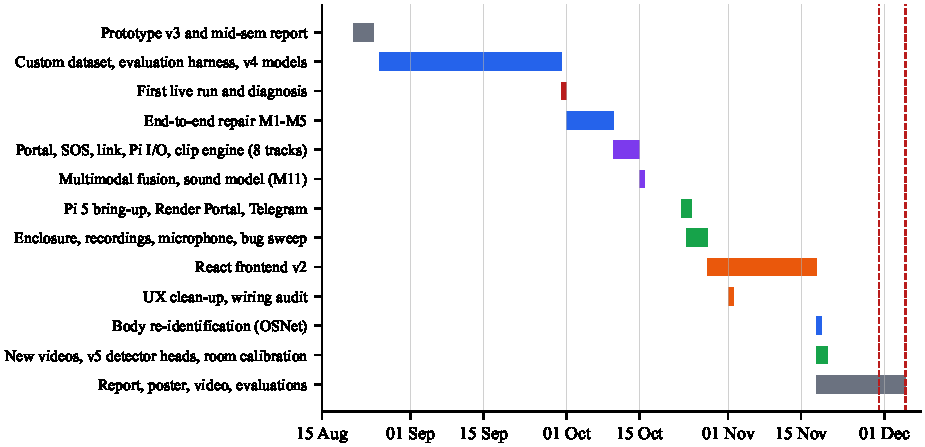
\includegraphics[width=\textwidth]{figures/fig_gantt.pdf}
\caption{Work schedule, August--December 2026 (dashed lines: evaluation on 30 November and final panel on 5 December)}
\label{fig:gantt}
\end{figure}

\section{Student Outcomes Description and Performance Indicators}
\tabref{tab:so} maps each student outcome and performance indicator of the course to the work in this project that demonstrates it.

\begingroup\tablefont
\begin{longtable}{|C{0.9cm}|L{5.5cm}|L{6.8cm}|}
\caption{SO1--SO7 mapping for the course UCS794 Capstone Project}\label{tab:so}\\
\hline\rowhead
\thead{SO} & \thead{SO Description} & \thead{Outcome}\\ \hline
\endfirsthead
\hline\rowhead
\thead{SO} & \thead{SO Description} & \thead{Outcome}\\ \hline
\endhead
\multicolumn{3}{r}{\footnotesize\itshape continued on next page}\\
\endfoot
\endlastfoot
1.1 & Ability to identify and formulate problems related to the computational domain & Identified that home alarms fail through false alarms, cloud dependence and lack of owner control, and formulated detection as committed alarm levels with measurable false-onset rates.\\ \hline
1.2 & Apply engineering, science and mathematics to obtain analytical, numerical and statistical solutions & Defined the evidence and TCI formulas, used Poisson and Clopper--Pearson bounds, ROC analysis and temperature scaling to choose and judge models.\\ \hline
2.1 & Design computing systems to address needs and build prototypes that meet design specifications & Designed and built the device, Portal, two web apps and the Pi~5 unit with enclosure against a written SRS and contract.\\ \hline
2.2 & Ability to analyse the economic trade-offs in computing systems & Compared edge and cloud inference costs, Pi 8\,GB vs 4\,GB, slim vs large models, and hosting options (Render vs Oracle).\\ \hline
3.1 & Prepare and present documents according to computing standards and protocols & Produced nine specifications, a decision log, an SRS following ISO/IEC/IEEE 29148, test documentation following 29119-3, and this report with IEEE references.\\ \hline
3.3 & Communicate effectively with peers using technical knowledge & Coordinated eight parallel tracks through a shared contract, code reviews and integration notes.\\ \hline
4.1 & Aware of ethical and professional responsibilities in computing solutions & Test mode by default, no automatic call to 112, consent of everyone filmed, data kept on the device, honest reporting of limits.\\ \hline
4.3 & Evaluate solutions considering environmental, societal and economic contexts & Assessed privacy under the DPDP Act, the societal cost of false alarms, energy of edge vs cloud, and the cost to a household.\\ \hline
5.1 & Participate in the development and selection of ideas to meet objectives & Proposed and compared fusion approaches, slim models and hardware platforms, selecting them by pre-registered criteria.\\ \hline
5.2 & Plan, share and execute task responsibilities in a team & Split work by subsystem and by track with clear ownership and milestones (M1--M11).\\ \hline
6.1 & Perform experimentation and analyse the results & Ran LOVO cross-validation, video replays, live and Pi benchmarks and re-identification experiments.\\ \hline
6.2 & Analyse and interpret data, make judgements and draw conclusions & Interpreted the room's score distributions to set thresholds, rejected the slim heads and the 0.50 re-id bar on evidence.\\ \hline
7.1 & Explore and utilise resources to enhance self-learning & Learned DINOv2, PANNs, OSNet, Picamera2, gpiozero, React and cloud deployment from papers, datasheets and documentation.\\ \hline
\end{longtable}
\endgroup

\section{Brief Analytical Assessment}
SENTRIX is a working end-to-end prototype of the product. Some items are still open: one interface defect (TC-29), Telegram delivery from the Render Portal to re-check, two release gates (G2, G4), and the Pi's 2\,s latency target. Its strongest results are in the system around the models: the evidence rules removed every false onset at Level~3 and above from the replayed live session and the labelled videos; the assistance flow handles the owner who approves, declines, is coerced or cannot answer; and the device keeps private data at home while the owner keeps control from anywhere. Its measured detection---9 of 12 handgun episodes and all flames at Level~3---comes from the team's own staged recordings, partly from training videos, and the false-alarm rate is bounded only loosely by the normal footage replayed so far, so it is evidence of feasibility rather than a validated rate. On the Raspberry~Pi~5 the product runs end to end but decides in about 4\,s rather than 2\,s. The project's main analytical contribution is its method: every claim is produced by a tool from committed data, model choices are fixed before they are tested, and limits are reported alongside results. The path to a validated product is clear: deployment-room recordings, a single detector trained on them, a fitted fusion model from real verdicts, and a hardware accelerator for the Pi.

%================== APPENDIX A: REFERENCES ==================
\clearpage
\addcontentsline{toc}{chapter}{APPENDIX A: REFERENCES}
\renewcommand{\bibname}{Appendix A: References}
\begingroup
\singlespacing\small
\setlength{\itemsep}{2pt}
\bibliographystyle{IEEEtran}
\bibliography{references}
\endgroup

%================== APPENDIX B: PLAGIARISM REPORT ==================
\clearpage
\chapter*{Appendix B: Plagiarism Report}
\addcontentsline{toc}{chapter}{APPENDIX B: PLAGIARISM REPORT}
The similarity report generated by the department's plagiarism-detection service for this report is attached on the following page(s).

\vspace{12pt}
\begin{center}
\fbox{\parbox[c][9cm][c]{0.85\textwidth}{\centering\itshape Plagiarism report to be inserted here\\(generated by the department on the final version of this report).}}
\end{center}

%================== SDG MAPPING REPORT ==================
\clearpage
\begingroup
\setstretch{1.2}
\setlength{\parskip}{7pt}
\begin{center}\textbf{\large SUSTAINABLE DEVELOPMENT GOALS (SDG) MAPPING REPORT}\end{center}
\addcontentsline{toc}{chapter}{SDG MAPPING REPORT}

\textbf{CPG No: 299}

\textbf{Project Title: SENTRIX -- Intelligent Multimodal Edge Threat Intelligence and Physical Security System}

\textbf{SDGs Mapped:}

\textbf{SDG 11 -- Sustainable Cities and Communities}

The project contributes to safer homes and neighbourhoods. SENTRIX detects armed intruders, fire and violent fights inside a home and brings the family's own contacts and a responder desk in within seconds of the owner's approval, or automatically when the owner cannot answer a serious alarm, while keeping false alarms near zero.

\textbf{SDG 16 -- Peace, Justice and Strong Institutions}

The project supports the reduction of violence and the protection of people in their homes. A duress PIN protects a coerced owner, and every alarm keeps tamper-evident, encrypted evidence and an auditable timeline of who was alerted and when. SENTRIX never contacts emergency services by itself and keeps personal data under the household's consent, in line with India's data-protection law.

\textbf{SDG 3 -- Good Health and Well-Being}

Fire and violence cause injuries where minutes matter. Early, confirmed detection of a visible flame or a fight, with the household's contacts and medical details reaching responders at once, shortens the time to help. Silence is never treated as safety: an unanswered alert is recorded as unanswered, and the safety defaults still reach the contacts.

\textbf{SDG 9 -- Industry, Innovation and Infrastructure}

The project shows that multimodal AI can run entirely on a low-cost single-board computer, without cloud GPUs and without sending video out of the home. Its open, measured approach---published decision rules, evaluation by alarm level, and per-room calibration---is a reusable pattern for affordable, privacy-preserving smart-home infrastructure.

\textbf{Technologies Used}

Edge AI (Raspberry~Pi~5), computer vision (YOLO, DINOv2, face recognition, OSNet), audio tagging (PANNs), multimodal fusion, AES-256-GCM evidence, FastAPI and React, Render, Telegram, e-mail and SMS.
\endgroup


\end{document}
